%!TEX root = ../../dissertation.tex
%%%%%%%%%%%%%%%%%%%%%%%%%%%%%%%%%%%%%%%%%%%%%%%%%%%%%%%%%%%%%%%%%%%%%%%%%%%%%%%%
\chapter{Mobile Core Network Investigation}
\label{chap:mobilenets}

The rise of reliable video streaming is not happening completely independent. Instead, it is deeply embedded into major shifts in Internet access. With more and more smartphones being used and even dial-up Internet access sometimes being replaced with stationary mobile \gls{3G} and \gls{LTE} modems. All these ``over-the-top'' streaming services are now being used within mobile networks.  

These cellular mobile networks are usually based on \gls{3GPP} specifications which have evolved from the circuit switched \gls{GSM} network into the fully packet switched \gls{LTE} which is still in its unrolling phase. But being packet switched does not mean that it shares a lot of similarity with a typical wireline Internet protocol stack and network infrastructure, for example a \gls{VDSL} or \gls{DOCSIS} dial-up connected to an \gls{IP} network. A ``3G'' network (a term synonymous for the typical type of cellular network used today) is very distinct from typical wired networks as it provides, amongst others, mobility and authentication in its lower layers through the core specifications rather than being optional on-top services as is typically the case in the Internet.

%% <-- WIP

The TCP/IP stacks largely follows two principles: \gls{KISS} and the end-to-end principle\cite{saltzer1984end2end}, which essentially means to restrict the protocols to the necessary bare-minimum and keep state only in the end systems. 3G takes a different approach, keeps a large amount of state at the obligatory nodes in its ``core network'', which explicitly communicate by signaling procedures defined by the \gls{3GPP}.
The adverse effects of state-keeping in network devices have been known to, e.g.,  Internet users running BitTorrent across low-end home routers as of the early 2000s. In \gls{UMTS} mobile networks, the networking hardware is vastly more powerful, but the control plane tasks are vastly more complex than port and network translation as well, namely carrying and routing IP and voice traffic, user mobility, \gls{AAA} and so on. Many specialized protocols are involved to communicate intents and states in the network. This causes processing overhead, additional traffic on network paths, and increases the number of states to be held in memory on the core network nodes. All of these attributes can be subsumed under the term network ``load'' which we plan to investigate in this work.


Given its roots as a research network and its growing pervasiveness over the last forty years, it is understandable that research on the Internet covers all parts of the network from applications to access to the core, and has been going on ever since what could be considered prehistoric times of the Net. The state of research on mobile cellular networks such as 3G is lean in comparison. Mobile networks providing Internet access have not been around for too long, and still are not available in all parts of the world. Furthermore, most research focuses on user-oriented metrics such as traffic statistics and mobility patterns, or takes into account the radio part of the network only. Little has been published about activity within the core network, and yet less about signaling.

Given how limited spectral resources on the radio interface are, it might not seem obvious to think about signaling load in the network. Yet, there have been situations where the core network unintentionally has been flooded with signaling, taking down user-plane connectivity on the way, despite small amounts of actual user traffic being transported \cite{lt2012docostorm, it2011birdandroid}. 

The adverse effects of state-keeping in network devices have been known to, e.g.,  Internet users running BitTorrent across low-end home routers as of the early 2000s. In \gls{UMTS} mobile networks, the networking hardware is vastly more powerful, but the control plane tasks are vastly more complex than port and network translation as well, namely carrying and routing IP and voice traffic, user mobility, \gls{AAA} and so on. Many specialized protocols are involved to communicate intents and states in the network. This causes processing overhead, additional traffic on network paths, and increases the number of states to be held in memory on the core network nodes. Therefore, in scenarios such as the ones mentioned above, radio access is not the bottleneck to connectivity any more, but signaling is.

%% <-- END WIP


This chapter is structured as follows. As it is absolutely necessary to get a grasp of the finer details of the mobile network architecture under investigation

\begin{itemize}
	\item Technical Background. Standards and Specifications. Network Architecture. Protocol Details.
	\item Dataset Description. Methodology.
	\item Definition of Load etc
	\item Evaluations. Dataset Analysis. Statistics. Traffic Characteristics. How does that user traffic fit in?
	\item Fitting, Modeling and Simulation
	\item Summary
\end{itemize}


%% <-- %% WIP
%% <-- %% end WIP

Core is usually neglected in communication investigations


While other publications look at the near-edge interactions in these network, research on the core is scarce, the reason for it being simple: you cannot do research without data from the operator there. Research at the edge, beginning at the IP stack level and upwards, can be conducted relatively simple. Writing simple tests and measurement scripts, often involving tcpdump and other tools, is usually all you need. But a mobile phone doesn't let you peek inside its layer 1 and 2 interactions (or even the implementation). Any information on this black box must be indirectly inferred from above (forcing behavior known from the specifications through scripts) or below (spectrum analysis using software defined radio approaches). To take a look at the core's view of traffic and data, one needs access to a dedicated measurement and capturing infrastructure placed inside the network. With this, researchers can not just look into user traffic flowing through the network but also quite easily into the signaling heavy mobile network control plane. 

Operators usually dimension their networks in relation to the occurring user traffic. But in such a signaling-dependent architecture this might not hold true anymore, as every user traffic has to be explicitly allowed, set up, and metered through all of the network's components. This has already led to some troubles in some mobile access networks, as heavy signaling for user traffic tunnels with very small amounts of traffic, that were however closed and reopened at a very high rate, caused an unintended \gls{DDoS} in the radio access network\cite{lt2012docostorm, it2011birdandroid}. 
This inherent complexity of signaling in mobile cellular networks is easily missed by programmers who do not or cannot know that their applications will run over such wireless links, and probably would not expect it from a network that pretends to transparently carry IP.

In this publication we attempt to give some insights into the mobile network control plane and its impact on dimensioning and load modeling. To do this, some important aspects of the \gls{3GPP} specifications have to be explained to give some basic vocabulary for the following exploratory research into signaling with a focus on \gls{PDP} Contexts and their management through \gls{gtp} tunnel management procedures. Using a week long data set from an Austrian mobile operator recorded at the Gn interface between the \gls{SGSN} and \gls{GGSN}, we attempt to find criteria influencing the signaling but we are also formulating hypotheses on the load impact of signaling, both backed by statistics gathered from the the data set.\\



%%%%%%%%%%%%%%%%%%%%%%%%%%%%%%%%%%%%%%%%%%%%%%%%%%%%%%%%%%%%%%%%%%%%%%%%%%%%%%%%
%% CoNEXT Intro starts here

The inherent complexity of signaling in mobile cellular networks is easily missed by programmers who do not or cannot know that their applications will run over such wireless links, and probably would not expect it from a network that pretends to transparently carry IP. What furthers this problem is the lack of literature on the theoretical and practical sides of these issues.

This apparent lack is due to a number of reasons. First, gaining sufficiently intimate knowledge on the huge corpus of \gls{3GPP} Technical Specifications %\gls{TS}
is a laborious task. Second, to come up with lower-layer measurements requires physical access to the core network infrastructure and suitable measurement equipment. Also, much of the data is commercially and privacy-sensitive, and cannot be published without extensive sanitizing.

The purpose of this paper will therefore be to give a 3G tunnel management primer, introducing the relevant \acrshort{GPRS}/\acrshort{UMTS} network structure and the involved control plane protocols with a special focus on the \gls{gtp}, which is probably the most prevalent. % We discuss how much overhead is put on the network through \gls{gtp} in a typical user traffic scenario.
Furthermore, we share our first insights into one practical aspect of the signaling process, the \gls{gtp} tunnel management procedures. Using a week long data set from an Austrian mobile operator recorded at the Gn interface between the \gls{SGSN} and \gls{GGSN}, % by the \gls{METAWIN} measurement infrastructure from the FTW, 
we take a look at \gls{PDP} Context durations, i.e. the time a \gls{PDP} Context is established and held, argue how this influences the load on the network, and evaluate the data by device types and operating systems.

Our measurement data backs up a number of straightforward assumptions on the behavior of different device and operating system types, but also reveals some remarkable differences in tunnel characteristics.\\





%%%%%%%%%%%%%%%%%%%%%%%%%%%%%%%%%%%%%%%%%%%%%%%%%%%%%%%%%%%%%%%%%%%%%%%%%%%%%%%
%!TEX root = ../../dissertation.tex
%%%%%%%%%%%%%%%%%%%%%%%%%%%%%%%%%%%%%%%%%%%%%%%%%%%%%%%%%%%%%%%%%%%%%%%%%%%%%%%%
\section{Background}
\label{c3:background}
%% reliable streaming
	%Web-based video streaming in general
	%Web, Flash, HTML5
	%relevance for mobile and future Internet
	%Drawbacks (no streaming, scaling, signaling, etc)
	%Internet Load and Video delivery performing with load
	%Example of YouTube
	%applicable quality metrics (normal metrics don't apply, no video quality scaling, observable only initial buffering time, stalls during playback, number, length, frequency thereof)


Before diving into the model some technical groundwork has to be laid. We describe protocols commonly used in the past and present and how to classify them. This is followed by other work related to this approach.

%%%%%%%%%%%%%%%%%%%%%%%%%%%%%%%%%%%%%%%%%%%%%%%%%%%%%%%%%%%%%%%%%%%%%%%%%%%%%%%%
\subsection{Definition} 

Any digitally stored video consists of a number of frames, organized into variable-sized groups, and audio samples which are played in sequence. Frames, single images of the video, do not only make use of typical spatial image compression mechanisms but encompass also temporal motion compensation, creating a dependence between frames. Videos can be encoded with a bit rate that is constant or variable over time. Typically, a variable bit rate encoding is chosen as these schemes offer a higher compression rate. To correctly display a frame, all previous frames in a block need to be present. 

Streaming, or to be more precise video streaming, is the process of playing a video while it is still being transmitted over a medium. As there is no need to have a file stored locally, received frames are typically put in a buffer to be played at the correct time. The amount of buffered video depends on the allocated buffer size as well as the video bit rate, and the transmission bit rate. It can also be controlled by the time offset between receiving the first frame of a video and actually playing it.


%%%%%%%%%%%%%%%%%%%%%%%%%%%%%%%%%%%%%%%%%%%%%%%%%%%%%%%%%%%%%%%%%%%%%%%%%%%%%%%%
\subsection{Streaming Classification}

Video streaming is a broad term covering a wide spectrum of applications as well as possible implementations. To break down and classify this field we define the following criteria to make a distinction.

\paragraph{Video Source}
The first criterion is the source of the video with the two major sources being a file stored on a remote server or a live source. Stored video can be streamed and played at any point in time. Live sources, on the other hand, are transmitting only at a fixed point in time. Depending on the type of content the timeliness of playback may also be important (imagine you are watching a game that is played right now).


\paragraph{Adaptivity of Content}
Video streaming can also be distinguished based on its adaptivity. In the simplest case there is no adaptivity present and the video is available in only one bit rate (which may still be a variable bit rate). 
But there are cases where an adaptation of the bit rate would be helpful. For example to accommodate for a clients needs in matters of the screen size. Usually, adaptation is used to tune the video stream to the currently available connection bandwidth. Adaptation can be achieved in two ways. Either to prepare and store several encoding levels beforehand or by encoding on-the-fly to a specific target. While the latter approach can adapt much more specific to certain goals it cannot be precomputed and will require more compute time when the number of clients becomes larger.

Adaptation also increases the amount of necessary control and information exchange. In the simplest case, streaming would only require a single command to start the streaming while any single adaptation adds another set of commands.


\paragraph{Location of Control} % Push-based (stateful) vs pull-based (stateless) vs network-controlled
Another matter is the location of control for a stream, with several possible ways to choose from. We distinguish between horizontal and vertical control.

In a horizontal direction control can be placed either at the streaming server, the streaming client or possibly somewhere in the network path in between.

A controller at the client typically just means that the video player itself is in control of the streaming process. The player starts the streaming and adjusts its requests to the server based on the player's needs. In this situation the server can be very lightweight as no decision logic needs to be present there. This is also called \textbf{pull-based} streaming.

Control can also be placed at the server with a stronger emphasis on the information available at the server side, making it easier to coordinate and adapt to a larger number of streaming clients. Similarly, this is called a \textbf{push-based} approach as video data is pushed to the recipient. 
For control to work properly state has to be kept imposing a certain memory overhead. This can become significant and a limiting factor for large streaming servers. Contrary, pull-based streaming usually does not require much or any state at all at the server.

Control information may need to be exchanged to communicate the state between the two endpoints. This can happen either explicitly through the exchange of signaling messages, or implicitly by drawing conclusions on another participants resources and behavior, for example through other protocols in the stack.

While not being able to control everything about streaming, the network may still be able to influence or manipulate an ongoing video stream. (Non-)Transparent proxies come to mind, which could intercept streaming requests and redirect them to another server located in the proximity of the requesting client.  A network can explicitly expose network's quality of service data to applications or these application can make reservation requests to the network.

Additionally control can be distributed vertically at different positions in the protocol stack. While usually streaming is conducted through a dedicated application layer protocol or even directly through an applications behavior, portions of control functions can also be offloaded to deeper layers. A typical example would be the use of \gls{TCP} for reliable streaming.

\paragraph{Reliability of Underlying Transport Protocol} % reliable vs unreliable
A major differentiation can also be made based on the reliability of streaming. Streaming can either act similar to a simple file download and just progressively download the video file in question while already playing it. This is conducted by using \gls{TCP} as a transport protocol, guaranteeing that no packet is lost in the process. \gls{TCP} does this by retransmitting packets it thinks are lost with the price of added latency and reduced throughput during retransmission. This reliability can however also cause the progress of the whole video stream to stall, If video data does not reach the client in time before its playback buffer is depleted, and therefore a perceptible loss of quality. This situation can be alleviated or even avoided by carefully planning the playback process and the buffering behavior.

On the other side stand streaming protocols that base themselves on \gls{UDP}, which offers no reliability features as \gls{TCP} and just sends out packets as-is. When packets are lost, the video can still progress but parts of the video output may be distorted or lost. Additionally, unreliable streaming protocols must take over other control features, that would otherwise have been taken care of \gls{TCP}. The adherence to an alloted or fair share bandwidth and congestion control come to mind, or else a high usage of this protocol could again lead to another congestion collapse \cite{rfc896}.

Transport protocols that offers congestion control but no reliable delivery might be a desirable middle ground between these two extremes. \gls{DCCP} \cite{kohler2006designing} is an example for such a compromise and might prove beneficial for the streaming process.


\paragraph{Multiplexing of Delivery} % multicast vs unicast vs maybe even broadcast
Finally, the number of targets of a single video stream can also differ. A stream is unicast if the control loop is exactly between one sender and one recipient. Servers can still support multiple unicast streams at once, they are just completely independent of each other. A multicast, or even a broadcast, stream is simultaneously sent to a group of recipients, stream control is established at the sender for the whole group. Therefore, multicasting is always using a push-based approach to control.


%%%%%%%%%%%%%%%%%%%%%%%%%%%%%%%%%%%%%%%%%%%%%%%%%%%%%%%%%%%%%%%%%%%%%%%%%%%%%%%%
\subsection{Survey of Protocols}

With these classification criteria at hand, we can now start looking at actual protocols, and find out, which motifs they are following. The section largely describe \gls{RTP} and compare it with \gls{HTTP}-based approaches including \gls{DASH} while also mentioning some other, proprietary, streaming protocols.


%%
\subsubsection{RTP and Related Protocols}

\gls{RTP} \cite{rfc3550} is always used in conjunction with its sister-protocol \gls{RTCP} and often also employs \gls{RTSP} \cite{rfc2326}. According to literature, they are the classic approach to video streaming (for example compare \cite[p.~589ff]{kurose2008computer} and \cite[p.~426ff]{peterson2007computer}).
The protocol suite employs a \textit{push-based approach}, the \gls{RTP} server application has full control of the streaming process. Control and information exchange is also out of band through \gls{RTSP} and \gls{RTCP}. Therefore, multicast is also easily possible with \gls{RTP} but not mandatory.

\gls{RTP} has also no inherent adaptivity nor reliability mechanisms, neither does it conduct congestion control on its own. Moreover, \gls{RTP} generally runs on top of \gls{UDP}, which also does not provide congestion control. All must be provided by the server-side application implementation if necessary. In case of multicasting the potential to conduct transport adaptations is very limited, as the server has to take all the recipients into consideration for its decisions.


\paragraph{RTP}

\gls{RTP} itself provides just the packet format and header for the transport of the actual multimedia data. Any stream type is transported in a separate session. This includes the presence of both video and audio, which must then be synchronized to each other. Each session uses its own \gls{UDP} source-destination port pair.

The \gls{RTP} specification itself defines only the most basic packet header, with several additional specs describing dedicated profiles for various content types. For today's prevalent MPEG-4 protocols, including H.264, multiple profiles, defined in \cite{rfc3640,rfc6184,rfc6416} , and with this many ways to embed video into RTP packets, are available. Common to all is the variable-size \gls{RTP} header of at least \SI{16}{\byte}. Video codecs may embed their own organizational structure inside the packet. For example, if dealing with an MPEG-4 \gls{ES}, the payload may contain one or more \gls{AU}.


\paragraph{RTCP}

\gls{RTCP} is used to exchange feedback and control information between receivers and sender and vice versa. These sender and receiver reports are transmitted on a separate \gls{UDP} connection at small intervals scaled in such a way, that the bandwidth should not exceed 5\% of the stream's bandwidth. The reports will include statistics related to lost packets and the packet delay and variation. Based on these, a sender can adjust its streams to fit the current conditions. Likewise, a receiver may tune its video buffering behavior or may even switch stream sources.


\paragraph{Stream Initiation}

RTP/RTCP itself provides no means to discover, initiate, and control the streaming process and has to rely on additional protocols. \gls{RTSP} is on of these, sitting atop of either \gls{UDP} or \gls{TCP}. It provides a set of commands the client can issue to a streaming server to control a stream and the streaming state at the server.

In case of multicasting, stream management can also be conducted directly by joining predetermined multicast groups through the use of \gls{IGMP} \cite{rfc4604} without the need for \gls{RTSP}.
This requires the cooperation of all intermediary routers. Therefore, it is usually only seen in closed networks (``walled gardens''), where the whole network infrastructure is owned by a single instance. For example, Telekom Austria's A1TV employs this scheme. \todo{reference, bernhard?}


\gls{RTP} is also used extensively in conjunction with a lot of other protocol suites, including \gls{SDP} \cite{rfc2327} and \gls{SAP} \cite{rfc2974} for stream discovery or in realtime communication protocols such as \gls{SIP} \cite{rfc3261} and \gls{XMPP} \cite{rfc6120,rfc6121} with the Jingle extension.

However, the requirement of several open \gls{UDP} sockets has issues with the presence of middleboxes, especially \gls{NAT} nodes, because of the difficulty to forward incoming \gls{UDP} packets to the destined host. This can be, sometimes though unreliably, circumvented by using \gls{NAT} traversal techniques like \gls{STUN} \cite{rfc5389} or \gls{ICE} \cite{rfc5245}.

%\gls{WebRTC} ZRTP, Secure RTP


%%
\subsubsection{HTTP Streaming}

When compared to \gls{RTP}, streaming based on \gls{HTTP} uses a much less intricate approach and only reuses existing protocols. HTTP/1.1 \cite{rfc2616} is the basis of the Web and is a request/response protocol mainly to retrieve and pull files from and to a remote location. The protocol is stateless for the server, any request is treated as standalone and will be responded to only with the provided metadata.\footnote{State can still be achieved through other paths, like cookies, but this is out of scope.} This holds true even when more than one request is sent over the same TCP connection, which can be done with persistent \gls{HTTP} connections. Additionally, requests can be sent over one connection without waiting for the answer of the previous request. This is called pipelining and can reduce the round-trip time delay between two consecutive requests.


But \gls{HTTP} can also be easily exploited for media streaming. The file to be retrieved should of course contain video and all frames have to be stored sequentially. If there are separate streams present in file, most commonly at least video and audio, they must be interwoven.
Necessary video metadata, which includes information on the codec and the streams, needs to be at the beginning of the file or at least before the position in the file where its needed. 
Alternatively, streams can also be stored in separate files, potentially simplifying the file structure. However, this increases the complexity of synchronizing both streams at the video player.

The actual streaming is controlled completely by the player application at the client. This player simply has to issue a \gls{HTTP} `GET'-request to a video file located at a Web server. The file can already be read during the transmission process and extracted video data will be put in the player's buffer. If there is enough video in the buffer, playback can be started. The complexity in this process comes from the need to keep track of the amount of video in the buffer and avoid to it run out at any point during playback. Approaches to this task will be explained in detail in Section~\ref{c3:sec:modeling}. \gls{HTTP} also allows so-called Range Requests, which allows to download only certain portions of a file, indicated by the Byte position. Streaming players can exploit this to enable skipping to certain positions. This again needs metadata to correctly infer the byte position in a file from the video playback position. Else, the Range Requests have to be guessed. 

%%
\paragraph{Reliability and Adaptivity}

\gls{HTTP} uses \gls{TCP} as transport protocol, which has implications to \gls{HTTP} streaming and makes it so distinct from \gls{RTP}/\gls{UDP}-based approaches. \gls{TCP}'s three large features are arguably reliability, congestion control, and flow control.

Reliability means, that at the transport layer and above no packets are lost and file requested by a \gls{HTTP} application will always be transmitted in full to the client (as long as the connection is not completely interrupted). \gls{TCP}'s sender side detects lost packets either by timeouts waiting for the corresponding acknowledgment or, preferably, through duplicate acknowledgments of previous packets. If either of this happens, the lost packet is retransmitted, causing a noticeably increase and variation in latency. But this also means, that the transmission of all consecutive packets has to wait on this one. On links with high loss the transmission can be stalled to such a degree that the incoming bitrate is lower than the bitrate of the playing stream, draining the buffer until it runs empty. Keep in mind, that with reliable streaming, frames, or parts of it, cannot be dropped, and the whole video will always be played.

In addition, \gls{TCP} also employs congestion control and avoidance mechanisms. While the sending rate of an \gls{UDP} application is completely controlled by the application's logic, \gls{TCP} detects and throttles the transmission to its fair share of the current connection. This can also cause the transmission rate to become lower than the video bitrate. The third transmission rate influencing mechanism is flow control. The receiver (and especially also the receiving application) can notify the sender, how much data it can receive in the next time window and thus can throttle the transmission rate itself.

This is an important method of control for the player. Usually, \gls{TCP}'s transmission fair share rate is expected to be much higher than the stream's video bitrate. While this makes sense for a simple file download to finish it as soon as possible, this behavior is unwanted for streaming. Rather, one wants to match the stream bitrate, with a bit of additional headroom to compensate for rate variations, to keep the playback buffer size in certain bounds that neither overwhelm the receiving device nor should the buffer be in danger of running empty. 

\begin{figure}[htbp]
\centering
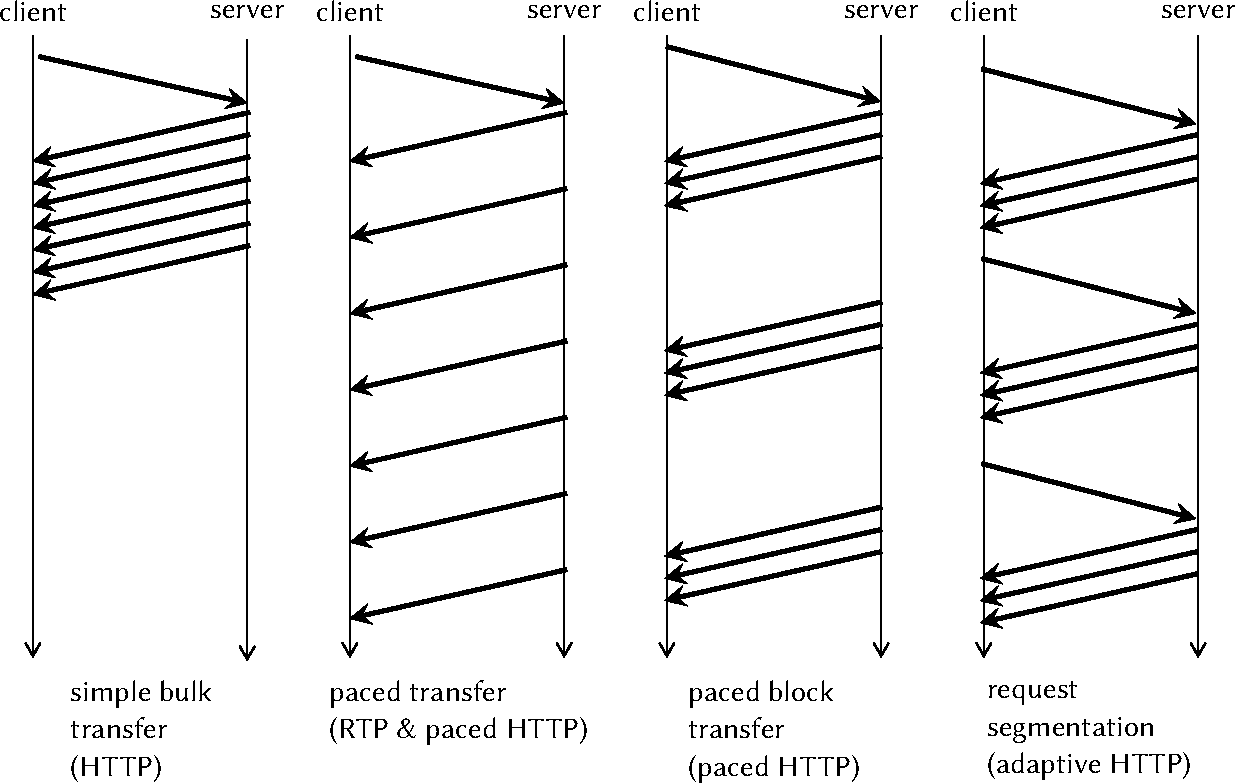
\includegraphics[width=1.0\textwidth]{images/streaming-transfer-modes.pdf}
\caption{Comparison of several possible streaming transfer modes \cite{ma2011mobile}.}
\label{c3:fig:streamingtransfermodes}
\end{figure}

\todo{reference to transmission pattern here? alternatively, put one of the old youtube throttling pictures here}

The first of the alternatives to achieve control over the playback buffer using \gls{HTTP}-streaming is to appropriately size \gls{TCP}'s flow control receive window by the application. 
Alternatively, the \gls{HTTP}-server can also manually throttle the download process, through various pacing strategies. The second and third transmission diagrams in Figure~\ref{c3:fig:streamingtransfermodes} depict two possible strategies compared to a regular \gls{HTTP} file transmission in the first transmission diagram. A third way, is to either partition the stream file into smaller even-spaced segments, that have to be requested independently, or use the aforementioned range requests on the stream's file. Through this, the receiving application can delay the request of new ranges or segments so that it matches a targeted bitrate over a longer timeframe.

These mechanism, however, can also result in a very bursty block-like transmission, a so-called ON-OFF pattern, and can cause undesirably interactions with \gls{TCP}'s flow and congestion control mechanisms \todo{ref to interaction}. Overall, stretching out the transmission may reduce server load spikes and the required buffer size on the client device but also makes streaming more vulnerable to insufficient network \gls{QoS} parameters. These specific approaches to pace to a target rate can generally be subsumed under the term \textit{Application Layer Flow Control}, which is also being implemented by some Web streaming services, e.g. YouTube \cite{alcock2011afcyt,metzger2011delivery}.

The aforementioned only adapt the transmission rate to the stream's bit rate and not the stream rate itself. Different video bitrates may be desired for many use cases, especially reacting to changing network conditions, take vertical handover from a 802.11 to a \gls{UMTS} network with a much lower throughput as an example. Quality adaptation with \gls{HTTP} streaming is generally achieved through the described range request or file segmentation mechanisms. For both approaches, multiple versions of the file or the segments have to be generated in different encoding quality levels. Also, the video file format needs to be able to support switching the stream and have an index to correlate the video files with their quality level and temporal position. \cite{ma2011mobile, watching-video1}

Several formal adaptive streaming protocols are in the process of standardization. \gls{HLS} \cite{pantos2011livestreaming} defines a playlist format to be stored separately on a server that links to all available stream variants and segments thereof in sequence. \gls{DASH} \cite{Stockhammer:2011:DAS:1943552.1943572} is a \gls{ISO}/\gls{IEC} \cite{iso-iec-23009-1} and 3GP-DASH \cite{3gpp.26.247} standard. Herein, all video segments are gathered in an alternative XML-based presentation scheme. Due to its file-based, using \gls{HTTP} for streaming is much more suited for stored video. But has also been successfully employed for live content, both \gls{HLS} as well as \gls{DASH} support this.


HTTP includes some support by the network in the form of proxies, but there are signaling methods that can e.g. forbid the caching of specific content through the no-cache directive \cite{rfc2616}.



\paragraph{Multicast}

No multicast, but can use CDN to almost the same effect.
	On the other hand, the rise of community pages like YouTube has shown, that the interest does not lie in watching the same content at the same time, but rather in high individualism. Therefore, multicast is less relevant for today's streaming. If there is a media event that is streamed live, one can always fall back to using the relatively new structures of \gls{CDN} to be able to serve large groups of users while still conserving bandwidth on the Internet backbones.


WebSocket\footnote{\url{http://www.websocket.org/}} \cite{ietf2011websocket} is a protocol running atop of \gls{HTTP} offering connection multiplexing and asynchronous as well as full duplex communication. It could be used to implement a more flexible \gls{HTTP} video streaming offering or unlocking further use cases. Similar approaches should be included and evaluated in the research for this thesis.

By using \gls{HTTP} the ideal platform for the client is either a plugin living inside a Web browser, the method chosen by Flash, or the browser itself, that in most cases has built-in video playback capabilities.

Location of Control: client-side and in-band ... but with websockets and SPDY / HTTP/2.0 could also be server side through server push

The capabilities and shortcomings of these novel mechanisms are not yet fully researched making it one of the prime foci of the thesis. Of special interest are:



%% <-- WIP




%%%%%%%%%%%%%%%%%%%%%%%%%%%%%%%%%%%%%%%%%%%%%%%%%%%%%%%%%%%%%%%%%%%%%%%%%%%%%%%%
\subsubsection{Other and Proprietary Approaches}

RTMP, ...

There are also other proprietary and standardized streaming systems which better fulfill the requirements of specific fields of applications. \gls{MBMS} \cite{3gpp22.146,3gpp22.246} is a specification defined by the 3GPP group for multicasting multimedia traffic specific to the architecture in mobile networks. But similar to \gls{RTP} the number of implementations and their acceptance are negligible.

The explicit control structure of protocol suites like \gls{IMS} \cite{3gpp.23.228} and \gls{MBMS} weaves application and network layer tightly together. This theoretically allows for an improved streaming performance at the cost of universally applicable behavior.

Peer-to-peer based approaches, including live-streaming!; describe P2P, 

%%

\begin{table}[htbp]
  \caption{Protocol Classification Matrix.}
  \label{c3:tab:streamingclassification}
  \tabulinesep=1.2mm
  \centering
  \begin{tabu}{|X|X|X|X|X|X|} 

  Protocol & \textbf{Location of Control} & \textbf{Reliable Transport} & \textbf{Video Type} & \textbf{Adaptivity} & \textbf{Multicast} \\ \tabucline[1pt]-\everyrow{\tabucline[on 1.5pt off 2pt] - }
  RTP &  &  &  & & \\
  simple HTTP & & & & & \\
  adaptive HTTP (DASH) & & & & & \\
  RTMP &  &  &  & &
  \end{tabu}
\end{table}


%% <-- %% end WIP
%%

%%%%%%%%%%%%%%%%%%%%%%%%%%%%%%%%%%%%%%%%%%%%%%%%%%%%%%%%%%%%%%%%%%%%%%%%%%%%%%%%
\subsubsection{Network Stack Layers and Streaming}
\label{sec:analysis}

In network layering models, it is often assumed that the layers are independent (or at least strongly decoupled) from, and only present narrow interfaces to, one another. From a conceptual point of view, media streaming is a process governing the application layer. Thus, the application and its behavior might be thought to dominate the overall streaming process and associated quality. In this Section, we will show that this is not necessarily the case.

Figure \ref{c3:fig:timescales} overviews the approximate time scales on which activities on different layers may take place, spanning a remarkable range of twelve orders of magnitude. Multiple layers might implement the same or similar functionality, e.g. flow control in the application and on transport layer, resulting in nested control loops, which might be coupled due to the timing constraints. 

\begin{figure}[htbp]
	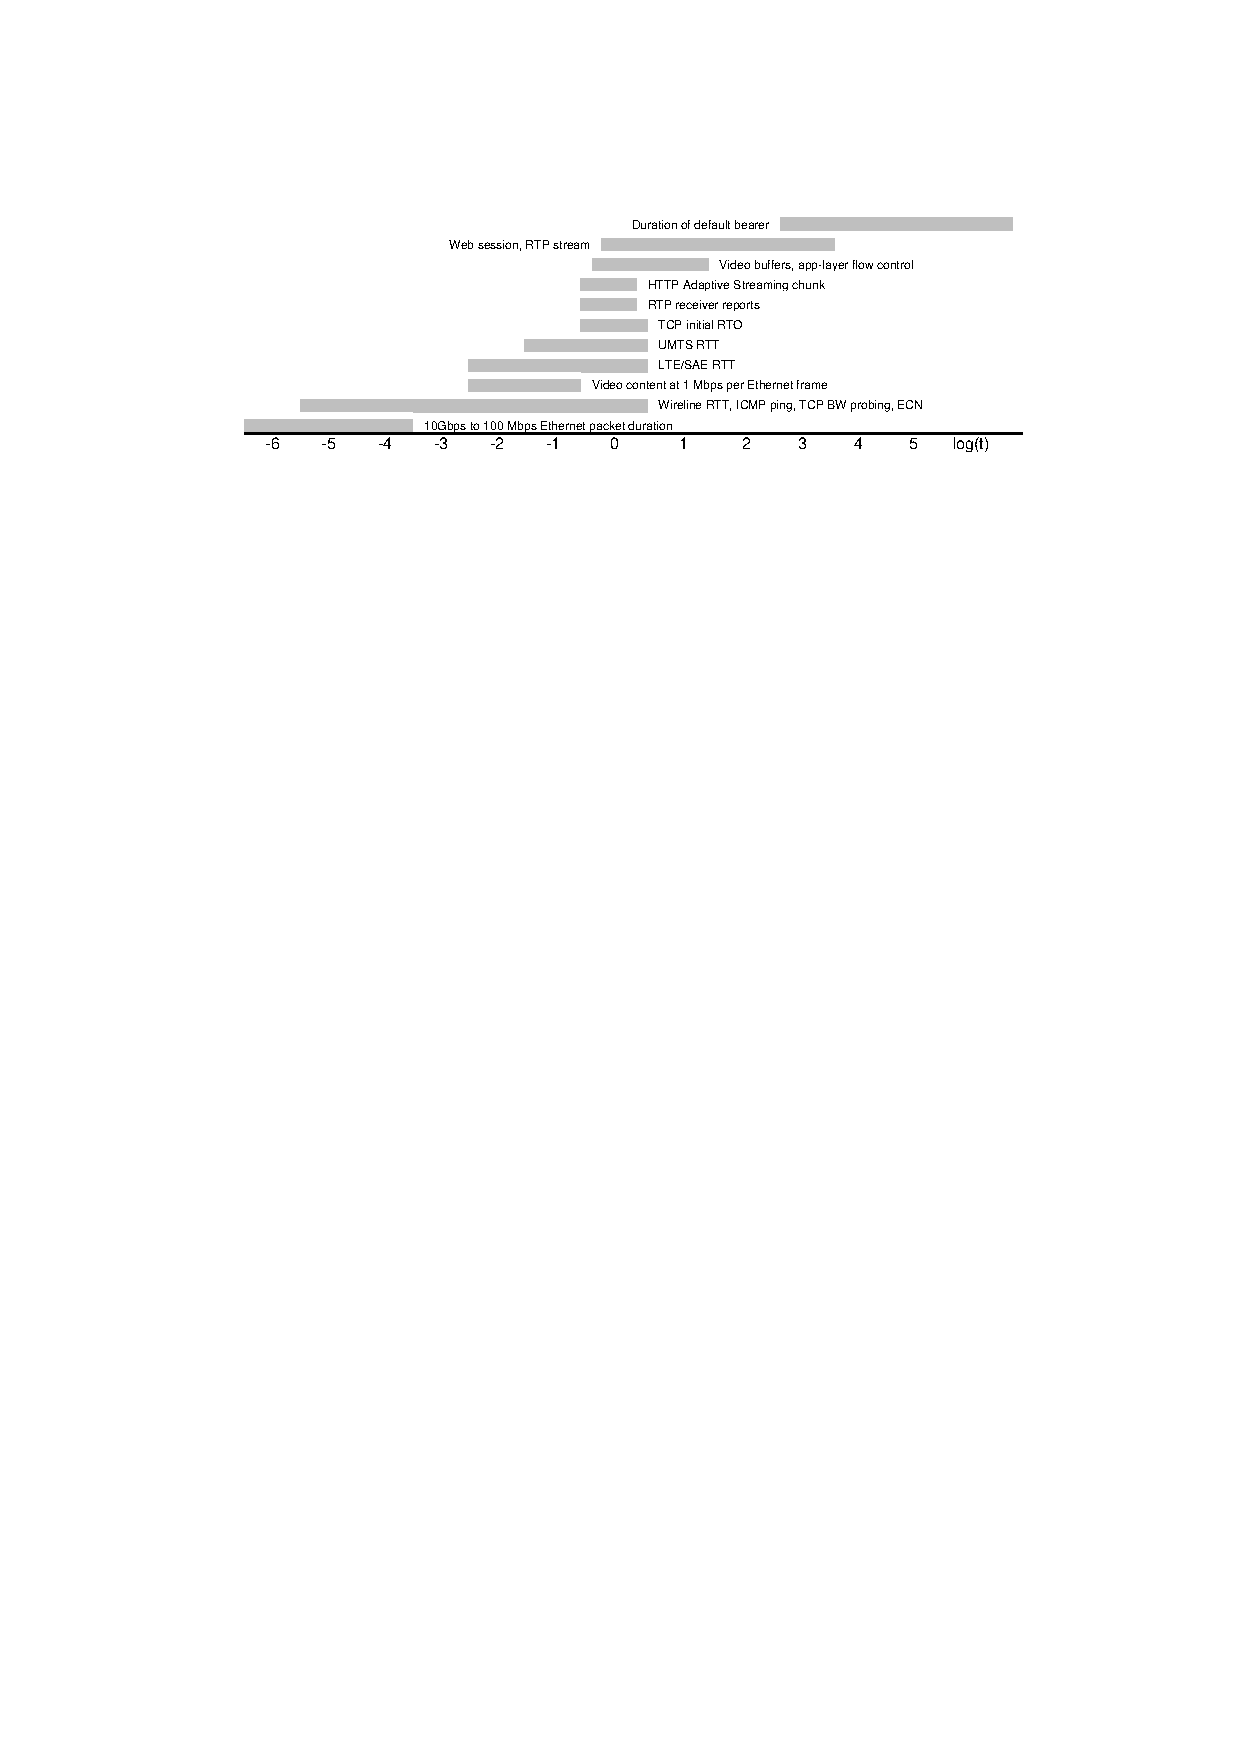
\includegraphics[width=\textwidth]{images/timescales.pdf}
	\caption{Relevant time scales in the layers of the stack}
	\label{c3:fig:timescales}
\end{figure}


\subsubsection{Network Layer}

As seen in Figure \ref{c3:fig:timescales}, the time constants found in different network implementations range from nanoseconds (for Gigabit Ethernet) to seconds (for UMTS and \gls{LTE}/\gls{SAE} wireless networks), depending on the technology used. This also influences the achievable round-trip time across such networks, which directly affects the performance of higher-layer protocols: \gls{IP}, \gls{ICMP}, \gls{UDP}, \gls{TCP}, and subsequently all application-layer protocols are all subject to these timing constraints.

In the case of wireless networks, typical effects of wireless connectivity relating to physical phenomena like fading and interference come into play. Flaky radio connectivity is a major source of packet loss and excessive delay. Certain cellular mobile technologies like \gls{UMTS} and its evolutions implement loss concealment themselves, confounding IP's assumption of a host-to-network layer lacking guaranteed delivery. Other peculiarities of cellular mobile networks include a \gls{MTU} opaque to IP, and delay variances as functions of packet sizes \cite{Arlos10} and radio access technologies \cite{laner2011dissecting}.


 Then, the technological progress enables both handsets and the network to become faster: Comparing the delay budgets given by x for \gls{UMTS} (2005) and y for \gls{HSDPA} R99 (2009) respectively, it is seen that the delay caused by processing on the mobile terminals decreased by a factor of 30, and that the core network has become faster by an order of magnitude as well. \cite{svoboda2006composition} has additional information on the delay budgets per network entity, varying the packet size as the parameter.
\gls{LTE} and \gls{SAE} also makes heavy use of the concept of bearers, a type of tunnel through the mobile network associated with quality levels and policy control. Although the bearer concept already exists in \gls{UMTS}, operators seem cautious to configure other bearers than the default one, and support by hand-sets is not widespread either. The setup procedure of \gls{LTE} bearers is sufficiently lengthy to be measurable and influence packet delay on initiating connections. 
\todo{re-insert references}
%
For reasons of radio spectrum efficiency, applications with long patterns of inactivity may be scheduled to not use HSDPA. This also causes measurable additional delay for applications [SVOB and their references 3 and 4].
%


\subsubsection{Transport Layer}

The two most widely used transport protocols are \gls{TCP} and \gls{UDP}. As is widely known, \gls{TCP} implements a number of elaborate mechanisms to establish and tear down connections, deliver data to the application in sequential order, conceal loss on the network layer, adapt its bandwidth usage to the capabilities of the other endpoint (flow control) and the network (congestion control), and share bandwidth fairly through a distributed control algorithm. Furthermore, its notion of ports adds a layer of addresses on top of the network layer.

UDP also supports port numbers, but does not include any of the other mechanisms \gls{TCP} has. This spurs the common misconception that \gls{UDP} is the faster transport protocol. In fact, all packet types are subject to the same round-trip time, independent of the transport protocol used. Delays in the delivery of data to the upper layer occur in \gls{TCP} when segments are considered lost in transmission (via timeouts or gaps in the range of acknowledged segments). \gls{TCP} retransmits the lost segments, causing the round-trip time to spike temporarily. In the case of \gls{UDP}, the application layer handles (or ignores) packet loss.

As indicated in the previously, mobile cellular networks often conceal packet loss, which is used by TCP as an indication for network congestion. Rather than lost, packets are highly delayed, which can cause sub-optimal bandwidth usage. Mobile networks also show artifacts relating to port and network address translation (commonly subsumed under \gls{NAT}), firewalling, and middleboxes interfering with \gls{TCP} timeout on long-lived connections \cite{sigcomm11middleboxes}.

\subsubsection{Application Layer}

There exists a diversity of streaming applications and associated application-layer protocols, each supporting to differing degrees certain types of streaming, and each having its own set of requirements, depending on the content type (pre-generated or live), the codec and its bitrate, and playback control and quality feedback.

One classification for streaming protocols might be their body of standardization: There are many proprietary protocols with undisclosed or legally restricted standards documents, e.g. \gls{RTMP}, \gls{MMS}, and \gls{WMSP}. Other protocols and protocol families are standardized by open bodies such as the \gls{IETF} In our work, we focus on these ``open'' protocols.

In the latter category are two well-known protocol families for media streaming, \gls{RTP} and \gls{HTTP}. \gls{RTP} sees most of its use in walled garden services such as IP TV. HTTP is the single most common application layer protocol on the Internet, owing its popularity to the ubiquity of web browsers. As \gls{RTP} is designed for media transport, a companion protocol suite consisting of \gls{RTCP} (for control information), \gls{RTSP} (for stream control like pausing), and \gls{SDP} (for session management) is often used. \gls{RTP} is mostly transported using \gls{UDP}.

In contrast to \gls{RTP}, \gls{HTTP} was not designed for specific payload types apart from \gls{HTML}. The actual streaming protocol behavior is defined by the application, not by the protocol. Every service is thus free to define its own distinct protocol behavior. For \gls{HTTP}, many de-facto variants for streaming exist, but many if not most are not formally standardized. There is work underway in the \gls{IETF} to create a standard for \gls{DASH}.



Within these protocol families, a multitude of implementations exist that suit specific demands. \gls{RTP} specifies an initial set of profiles (RFC3551 \cite{rfc3551}), with a multitude of definitions cropping up with every new type of media coding scheme . In HTTP, the actual transfer model, addressing, and metadata mechanisms have been in place virtually unchanged since 1999, when HTTP/1.1 was specified. Much innovation has since gone into the payloads transferred via HTTP, as well as the control of its underlying transport protocol, TCP.

Both protocol families offer a wide range of techniques, established and recent, de-facto and formally standardized, each supporting different types of streaming and content, and each subject to the interplay of content requirements, the application, the network, the media player, the layer stack, etc. Seemingly, not one single protocol can solve all problems at once. 

The Real-time Transport Protocol (RTP) \cite{rfc3550} is an IETF protocol designed for (near) real-time payload such as multimedia or sensor data. It is designed for support by the network. \gls{RTP} supports mixers and translators that enable transcoding of content as it travels through the network.

Since RTP is typically transported over UDP, it is also multi-cast compatible. For example, A1 Telekom Austria’s A1TV uses an Organization-local cope Multi-cast \cite{rfc2365} tree with distinct IP addresses for each program. At the same time, \gls{UDP} is not inherently congestion-controlled, and \gls{RTP}'s own congestion control mechanism (if activated at all) has a relatively long delay to respond for reasons of rate limiting on the control channel. This means a wide-spread use of \gls{RTP} could even cause congestion collapses in parts of the network.



\subsubsection{Protocol Comparison}
In \gls{RTP} streaming, it is customary to have multiple flows for different parts of the media stream, e.g. audio and video, and a separate control connection. In \gls{HTTP}, one (or multiple consecutive) TCP connection is used for both control and data transfer.
In \gls{RTP}, flow control on the transport layer needs to be done by the server application. The same goes for congestion control, which is implemented using receiver reports, or might be left out altogether. HTTP uses TCP as its transport protocol, and thus inherits its flow control and congestion control features.
There are several implementations for application-layer flow control. Simple bulk transport is the typical web download model, which assumes that both the client and the server try to transfer the data as fast as possible. Contrarily, paced transfer is implemented by \gls{RTP}, where the server sets the bitrate the client will see. An interesting variant on paced transfer is paced block transfer, implemented for example in the YouTube block sending mechanism. The specific incarnation consists of server-controlled burst sending of 64kB blocks and inter-block gaps of variable length to adjust the download rate to the average video bitrate. An additional initial burst phase is present to prefill buffer.
 
Playback control is actually done by the server in the case of RTP, where the client issues requests to, e.g., pause the stream, and the server then reacts. In HTTP, the client is in much stronger control of the playback, and need not notify the server of a user's decision to skip backwards, etc. 
For the exchange of transport control information such as packet loss, RTP uses a companion protocol named \gls{RTCP}. HTTP again leverages TCP, where such information is exchanged implicitly. It must be noted however that due to the flexible data format RTCP pro-vides, more concise information can be signaled in addition to transport control related matters.
To conclude, the different protocols are also specified to different degrees. As stated before, there is a large body of \glspl{RFC} relating to RTP and its adaption to new media, content, etc. For HTTP, many de-facto used variants adapted to streaming exist, but many if not most are not formally standardized. There is work underway in the \gls{IETF} to create a standard for \gls{DASH}.



% \begin{figure}[htbp]
% \centering
% 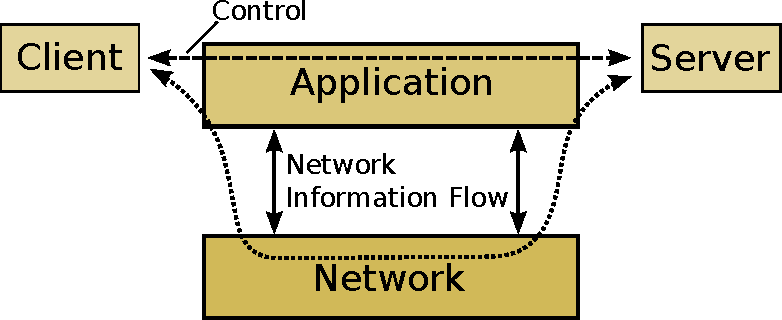
\includegraphics[width=0.8\textwidth]{images/nif.pdf}
% \caption{Theoretical information exchange paths between streaming partners.}
% \label{c3:fig:nif}
% \end{figure}

%One future trend is said to be an increase in the required communication confidentiality and authentication. One of the goals might be to enable full end-to-end encryption on the transport level of the network. This could be achieved either by providing an encrypting alternative to TCP, e.g. CurveCP \cite{curvecpwww} and TCPCrypt \cite{tcpcrypt}, or by using HTTPS and moving other functionality further up the stack.


% \subsubsection{Video Delivery Architecture}
% \label{c3:sec:videodeliveryarchitecture}
% Large Internet sites are not hosted at one central site anymore, but are usually served through geographically distributed entities forming a load-balancing structure. Such load balancing mechanisms have a long history on the Web, e.g. in the form of mirror servers a user can select manually.

% In today's Content Distribution Networks (CDN), a much larger number of mirror servers is available, and selection of a server is no longer carried out explicitly by the user, but implicitly through DNS: Content is addressed using URLs (\texttt{http://somedomain/somepath} in its simplest form), and the CDN's DNS servers are configured to resolve certain domain names to different IP addresses, depending on where the query originated.

% To get an insight into the structure of YouTube's content distribution network, we undertook a two-step measurement campaign \cite{rafetseder2011explyt}. First, we downloaded and manually parsed the HTML code served by YouTube's web servers. We could thus enumerate and learn about the structure of domain names in the system. The most relevant category of domain names for our purposes takes the form of \texttt{v$\alpha$.lscache$\beta$.c.youtube.com}, where $0<\alpha<25$ and $0<\beta<9$. Not all permutations of names are found at all times. We also noted that there are hostnames that seem to point to geographical locations, but have not succeeded so far in exhaustively mapping those two types of names.

% The second part of our campaign consisted of active measurements on forty distributed computers (part of the \textit{Seattle} Internet testbed\footnote{\url{https://seattle.poly.edu/html/}} \cite{Cappos:2009:SPE:1508865.1508905}) for over 600 hours. We learned that the frontend web server name, \texttt{www.youtube.com}, resolves to multiple IP addresses per geographical location of the probing host which are mostly disjoint from sets of addresses found on other hosts. The number of frontend IP addresses also changes over time, e.g. to account for load variations such as load increases during the evening hours in the hosts' time zones. The actual video cache servers only have one IP address per name and location each, but sometime this address is seen to change during the day. 

% When looking at the resolved addresses per frontend server and time zone, two interesting time-dependent scaling effects can be seen: First, servers become reachable or vanish in a coordinated manner controlled by the time of day, i.e. in a 24 hour pattern. We speculate this provides a gain in efficiency for the overall system to turn on parts of the resource pool for load balancing only when there is demand.

% The second type of effect occurs much more seldom. It stretches out over multiple days and is best described as follows: A new block of server IP addresses is made available in addition to the existing ones. After a few days of parallel operation, a previously active block is taken out of service. The new block continues to serve. Comparison measurements  performed in parallel show that this switch-over between IP address blocks has a positive effect on the latency to the servers, as the latency to non-YouTube destinations show no improvements at all.

%%%%%%%%%%%%%%%%%%%%%%%%%%%%%%%%%%%%%%%%%%%%%%%%%%%%%%%%%%%%%%%%%%%%%%%%%%%%%%%
%!TEX root = ../../dissertation.tex
%%%%%%%%%%%%%%%%%%%%%%%%%%%%%%%%%%%%%%%%%%%%%%%%%%%%%%%%%%%%%%%%%%%%%%%%%%%%%%%%
\section{Related Work}
\label{c4:sec:relwork}

The investigations conducted in both this and the subsequent chapter do not fall strictly into an existing research category but instead aim to provide diverse insights into the control plane from the perspective of the core network. Nonetheless, a selection of publications from the tackled fields is collected here and the interesting aspects for this work are noted. In the following sections the related work is divided into four distinct fields.

Work in the first and second sections evaluate properties of the mobile network and its traffic. They are distinguished in their approach to the investigation, as the first group uses active measurements from mobile devices or conclude from other sources of traffic whereas to the other one has access to passive measurements from inside a \gls{3G} mobile network. Publications from the third category can be generally subsumed under the term \textit{traffic modeling} and may not be specific to cellular networks. The final field concerns itself with investigative work conducted by the responsible standardization and organizational bodies themselves, i.e., the \gls{3GPP} and \gls{GSMA}.


%%
\subsection{Device Active Measurement Investigations}

The approach taken by active measurement studies is simple yet still very insightful. They are performed by writing custom application layer measurement programs for a mobile device. Specific traffic patterns are then generated, recorded, and evaluated. While this can provide very detailed information about the higher network layers, it is limited both in lower layer information as well as scale, due to being limited to a rather low number of devices.

Despite being more or less completely specified in the \gls{3GPP} documents, there is no open layer 1 and 2 (together also called ``baseband'') implementation for \gls{3G}.\footnote{Apart from OsmocomBB (\url{http://bb.osmocom.org/trac/}), but it only provides \gls{GSM} and partial \gls{GPRS} functionality.} Therefore, the baseband's behavior can not be directly instrumented from the application layer. Attempts to infer some properties are still worth conducting as the following selection of publication demonstrates.

In~\cite{Xu:2011:CDN:2007116.2007149} Xu et al.\ use data from a location service combined with active measurements to determine the possible geographic location of a \gls{GGSN} in order to improve the location of application content caches for the current network infrastructure. Similarly, in \cite{sigcomm11middleboxes} Wang et al.\ developed a program to probe mobile networks for middle boxes. That term includes any node, that alters traffic and affects performance not intended by the actual end-to-end protocols. Examples are \gls{CGN}~\cite{rfc7021}, firewalls, or intercepting \gls{HTTP} proxies. A large number of such nodes were present in the investigated mobile networks and resulted in increased device power usage and download durations and even pose security issues themselves.

Concerning methods to infer specific baseband and \gls{RRC} state machine timer values with active measurements, a 2007 paper~\cite{4640935} presents a way to do this by transmitting packets with a varying inter-departure time and studying the resulting arrival pattern. Indeed, the dynamics of the radio interface's \gls{RRC} signaling and involved state machines are under investigation by several publications. However, almost all focus solely on the impact at the radio interface but pay little attention to potential implications in the \gls{CN}.

The aforementioned work is continued in \cite{5360763} and uses the presented tools to derive \gls{RRC} transitions and power usage from traffic patterns. They found, that operators have a rather larger freedom in configuring the mobile network control plane state machines and deviate from the standard and even omit some states completely.

A further example of cross-layer influences in mobile cellular networks is \cite{qian2011profiling}. It discusses the impact of application layer behavior on \gls{RRC} signaling and its consequences for device energy consumption and radio channel allocation efficiency. The authors argue that there is much room for improvement in this area, and propose some enhancements.

This is further elaborated on by research from Schwartz et al.\cite{schwartz2013angrybirds} using the same technique to analyze the radio signaling load and thus power efficiency from several mobile phone applications. The impact of custom set state machine timers interacting with application traffic is further investigated and the \gls{QoE} is investigated.


%%
\subsection{Research Based On Network Traces}

The second alternative to mobile network investigations comes in the form of recording and evaluation traffic traces inside the network. This brings a much larger experiment scale with it, albeit usually at the cost of some finer grained details in the higher protocol layers because of aggregation to flow level. With core network measurements, the signaling traffic of the observed link can also be directly investigated, which is a huge benefit compared to the guesswork in active measurements.

The authors of \cite{4675847} investigate the influence of individual \gls{CN} nodes on the one-way delay distribution of user traffic packets. According to the work, the latency portion added by the \gls{SGSN} is larger but also fluctuating more, while the \gls{GGSN} added a small but steady amount of latency. This provides us with initial clues on the expected load impact of the \gls{CN} for the investigations in this work.

Following up on the topic of mobile network one-way delays is Laner~et~al.\ in \cite{laner2012delaycomparison}. The end-to-end latency of an early \gls{LTE}/\gls{EPC} network implementation is compared to that of a \gls{HSPA} network at several measurement points in the networks. The results show a lower median latency for \gls{LTE}, despite some scenarios still being in favor of \gls{3G} networks.

The authors of \cite{Shafiq:2012:FLC:2254756.2254767} limit their focus to a specific subset of connected devices, namely those of \gls{M2M} type. These are small automated devices, that periodically send out data, e.g., sensor readings, or receive control commands. The paper attempts to characterize these on the basis of their generated mobile network traffic. The patterns are clearly distinguishable from traffic caused by other device types such as smartphones.

A 2012 publication~\cite{Zhang:2012:UCC:2377677.2377764} presents us with a more general look on the traffic composition of cellular access networks in comparison to wired access network. Much more and shorter flows are occurring in the case of cellular networks. It will be interesting to see if this shorter-but-more theme is also evident in signaling traffic. Additionally, even traffic pattern distinctions between types of applications are made showing a wide range of possible outcomes across the investigated applications.

Both the authors of \cite{shafiq2011characterizing} and \cite{paul2011understanding} take the approach of looking at high-level user traffic characteristics in a mobile network, focusing on temporal and spatial variations of user traffic volume and peeking at the influence of different devices on this metric. Additionally, \cite{baer2011two} delivers a theoretical introduction on how to conduct large scale network measurements and compares some data evaluation approaches. The 2008 paper of \cite{4570772} takes a look at times scales and time of day deviations observed in aggregated user traffic in a mobile network.

Up until now no trace-based investigation considered the control plane in their evaluation. The following publications include this at least to some degree.

In 2006, Svoboda~et~al.~\cite{svoboda2006composition} conducted a core network measurement study of various user traffic related patterns, and also provided an initial insight into \gls{PDP} context activity and durations. Another paper~\cite{lee2007detection} combines simulations based on WiFi and synthetic traces with prior knowledge of \gls{RRC} states and their effects to investigate detection methods for signaling \gls{DDoS} occurring on the radio interface. A possible magnitude of this type of attack is discussed. This also gives an indication of the correlation between user traffic patterns and radio signaling.

A 2010 publication\cite{Qian:2010:CRR:1879141.1879159} uses the indirect \gls{RRC} inferring method described earlier on a core network \gls{TCP} trace data set and finds that the involved \gls{RRC} state machine is largely inefficient in terms of signaling overhead and the device's energy consumption for the traffic patterns seen in the data. 

A more recent publication at \cite{he2012panoramic} performs a \gls{RRC} investigation at the path between \gls{RNC} and \gls{SGSN}. The authors classify their evaluations based on device model and vendor and on the application type, and find that different devices have strongly different \gls{RRC} characteristics, which could possibly also have an impact on \gls{gtp} signaling. Here, the \gls{RRC} evaluation was done in a direct manner using explicit logs from the \gls{RNC}. A final paper~\cite{Ricciato2010551} recaps some general attack scenarios on \gls{3G} networks that exploit the specific \gls{3GPP} system design. These are often closely related to the control plane.


%%
\subsection{Traffic Modeling}

Extracting viable models from mobile traffic measurements will also play a significant role. The first related work is a survey of source modeling approaches for \gls{GPRS} user traffic from the year 2000 \cite{staehle2000source}. Models for \gls{HTTP} traffic and user behavior are compared and a combined model is recommended. One has to keep in mind, though, that due to the rapid developments in the Web in recent years those models might no longer be valid. 

Similarly, the authors of \cite{965876} derive a synthetic \gls{UMTS} traffic model from wired dial-up traces. By using a batch Markovian arrival process they characterize session traffic in most cases with a lognormal distribution.

Work conducted in \cite{Halepovic:2005:CMU:1089803.1089969} derives a model for the users' mobility in a mobile network. The mobility model is however more focused on the circuit-switched voice communication features of a phone. Likewise, the authors of \cite{Pesch2005385} introduce a traffic model for \gls{SIP} \gls{VoIP} communication in \gls{UMTS} networks. However, this model is specific to the \gls{IMS} domain of \gls{UMTS} and potentially not applicable to the more common over-the-top pure \gls{SIP} traffic. But the model additionally investigates some initial \gls{UMTS} control plane timing values, such as the processing time of \gls{PDP} context activation messages.

A further publication in 2005 \cite{Landman200568} attempts to model the delay of \gls{IP} packets passing through an \gls{UMTS} network using a batch Markovian arrival process. However, the model specifically focuses solely on the delay originating from processing at the radio link and not at the core nodes.

Finally, a further paper by Laner~et~al.~\cite{6214330} investigates, amongst other things, a user's session duration and throughput in a \gls{HSDPA} network. The duration is modeled as an exponential distributions and the throughput using a lognormal distribution, albeit both exhibit additional heavy tail characteristics.


%%
\subsection{\texorpdfstring{\acrshort{3GPP}}{3GPP} and \texorpdfstring{\acrshort{GSMA}}{GSMA} Related Work}

The two associations related to the mobile network under scrutiny, the \gls{3GPP} as well as the \gls{GSMA} themselves have also released some studies and recommendations concerning potential effects of and issues with the control plane. 

In reaction to the mentioned \gls{RRC} signaling \gls{DDoS} the \gls{GSMA} released some best practices \cite{gsma2011fdbestpract} intended to reduce the number of signaling messages in these circumstances. The cause of the \gls{DDoS} were in most cases mobile devices, that circumvented the \gls{RRC} state transition timers and explicitly switched the radio to the idle state after a transmission was finished and re-enables it whenever needed. This can greatly reduce the power usage but increases the number of signaling messages to be sent and thus the load in the radio network and possibly also inside the \gls{CN}. With the presented ``Fast Dormancy'' mechanism, mobile devices are supposed to reduce the radio signaling amount while still saving energy. The implications of this mechanism on the core are not investigated.

A \gls{3GPP}-released study \cite{3gpp.22.801} also describes the diverse traffic mix originating from modern smartphones and its associated signaling problems.

The aim of the study in \gls{TS}~23.843~\cite{3gpp.23.843} is to document some of the control plane bottlenecks and attack vectors on the \gls{CN}. This also includes the interesting case of \gls{GTP-C} overload and causes for this scenario. Some approaches to alleviate the effects are also presented but mostly targeted at the \gls{EPC}. The final study is an extension to the last one \cite{3gpp.29.807} and focuses solely on \gls{GTP-C} overload control to be included in a future version of the \gls{3GPP} architecture. Therefore, the mostly unfinished document again targets just at a future version of \gls{LTE} and provides no investigation of the actual load situation in current \gls{3G} networks.

All of the presented publications relate to some degree to this chapter. However, the combination of the aspects of \gls{CN} signaling with a statistical evaluation and load modeling of \gls{PDP} contexts should be a genuine contribution of this chapter.



%24.826 \cite{3gpp.24.826} Study on impacts on signalling between User Equipment (UE) and core network from energy saving; deals mostly with switching off cells and moving over UEs, not actual core network efficiency

%%%%%%%%%%%%%%%%%%%%%%%%%%%%%%%%%%%%%%%%%%%%%%%%%%%%%%%%%%%%%%%%%%%%%%%%%%%%%%%
%!TEX root = ../../dissertation.tex
%%%%%%%%%%%%%%%%%%%%%%%%%%%%%%%%%%%%%%%%%%%%%%%%%%%%%%%%%%%%%%%%%%%%%%%%%%%%%%%%
\section{Evaluation Methodology}
\label{c4:sec:methodology}

With the mobile network load defined and possible influencing factors described, the findings can now be applied to an actual mobile network. For this data from passive network traces will be employed. But first, the monitoring setup and the captured has to be described in this section. This also includes a description of some methods required to examine specific device types and other device-based factors from the dataset.

While this chapter only employs passive measurements, Chapter~\ref{chap:mobilestreaming-measurements} will additionally deal with approaches to conduct meaningful active device-based measurements and set up a mobile streaming simulation testbed based on some of the results.


%%%%%%%%%%%%%%%%%%%%%%%%%%%%%%%%%%%%%%%%%%%%%%%%%%%%%%%%%%%%%%%%%%%%%%%%%%%%%%%%
\subsection{Network and Monitoring Setup}

For the analysis, the \gls{METAWIN} monitoring system developed in a previous third-party research project and deployed in the network of an Austrian mobile operator is used. Detail information on this setup can be found in \cite{ricciato_2011,ricciato2006traffic}.

\begin{figure}[htb]
	\centering
	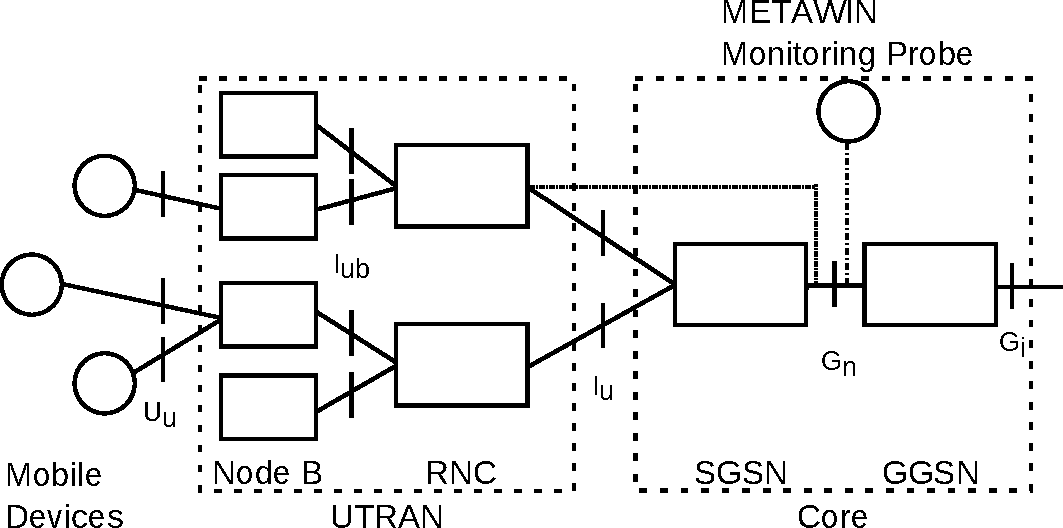
\includegraphics[width=0.7\textwidth]{images/umts-network.pdf}
	\caption{Location of the \acrshort{METAWIN} monitoring probe in the \acrshort{3G} core network.}
\label{c4:fig:umtsnetwork}
\end{figure}

The measurement taps are located at the Gn interface at one \gls{GGSN} within the core network as depicted in Figure~\ref{c4:fig:umtsnetwork}. It gives access to a wide spectrum of core \gls{gtp} signaling, including the mobility and tunnel management. The system does not offer a complete packet trace, but aggregates every signaling transaction and user traffic flow down to a number of select fields. This includes \gls{gtp} \gls{IE} such as the \gls{RAT} as well as the terminal types of the mobile clients. The latter is determinable by the \gls{TAC} part of the \gls{IMEI} and will be discussed later in detail.

In the network under study, a direct link between \glspl{GGSN} and the \glspl{RNC} and circumventing the \gls{SGSN} is present. It is only used for transporting user-plane traffic under specific circumstances, and signaling procedures are still carried out in the normal way between \glspl{SGSN} and \gls{GGSN}. Therefore, only the Gn interface at \gls{GGSN} is seeing the complete core network traffic, which explains the location of the tap. The network under study has more than one \gls{GGSN} at different physical locations. The tapped \gls{GGSN} manages about half of the operator's total traffic volume in this period. 

Recording data in a live network necessitates meeting strict privacy requirements regarding the handling of user-related data. \gls{METAWIN} complies with this by anonymizing all user-identifying. Application-level payload is removed and all user identifiers (e.g. \gls{IMSI}) are non-reversibly hashed before recording. \glspl{UE} in a dataset can still be differentiated by the hashes but not traced back to the actual user. The wiretaps deployed within the monitoring system are time-synchronized with \gls{GPS}. Accordingly, the packet timestamps have an accuracy of least \SI{100}{\nano\second}.


%%%%%%%%%%%%%%%%%%%%%%%%%%%%%%%%%%%%%%%%%%%%%%%%%%%%%%%%%%%%%%%%%%%%%%%%%%%%%%%%
\subsection{Dataset Description}

Using \gls{METAWIN} a week-long core trace was acquired. It was recorded in April 2011, specifically beginning at Monday, \yyyymmdddate\formatdate{10}{4}{2011}, \formattime{0}{0}{0} and ending Sunday, \formatdate{17}{4}{2011}, \formattime{23}{59}{59}.

The trace includes user plane as well as control plane traffic. User plane traffic is recorded in a traffic flow granularity with the trace containing data on \num{2.2e9} aggregated flows. No exact flow start time is given, instead it is rounded down to a \SI{2}{\hour} window with the timestamp at the beginning. A flow entry further consists of hashed identifiers for the gls{IMSI} and the remote server. Besides the usual protocol and port information, the transmitted data volume, in a number of packet as well as byte count, is given on in both link directions. Additional information is available on \gls{HTTP} traffic. This portion of the trace includes precise timestamps as well as the \acrshort{MIME}-type, result code, and size of the requested objected.

The recorded control plane traffic consists of \num{4.1e8} \gls{gtp} tunnel management transactions, i.e., every create, update, and delete request and response. Not all of the \glspl{IE} data is included. But most importantly, it includes the \gls{TAC}, \gls{RAT} and hashed \gls{IMSI} for the purpose of device discrimination. Also present are several timestamps with \SI{64}{\bit} precision describing the time of the request, response and the tunnel's start time. Finally, the \gls{gtp} data contains the response codes for each request. With these codes, failed transactions can be distinguished from successful ones and examined separately. Since the hashed \gls{IMEI} is consistent across the user and control plane data, both can be cross-correlated.

All trace information was exported from \gls{METAWIN} as pure line-based text data. For this investigation all records were fed into a \acrshort{SQL} database. Evaluations were conducted through scripted queries on the database using Python scripts and further statistically evaluated in R.

%%%%%%%%%%%%%%%%%%%%%%%%%%%%%%%%%%%%%%%%%%%%%%%%%%%%%%%%%%%%%%%%%%%%%%%%%%%%%%%
\subsection{Device Identification}

Individual device types in a mobile network can be identified in the data through the \gls{TAC} field on every entry. The \gls{TAC}, defined in \cite{3gpp.23.003}, represents the first eight decimal digits of the \gls{IMEI} and uniquely identifies each device type. The following six digits of the \gls{IMEI} constitute the serial number of a specific device, which is of course omitted in the data. Due to the short length of this serial number, popular devices will often be assigned more than one \gls{TAC}, somewhat complicating the identification of certain device models.

\glspl{TAC} are assigned to individual device models by the regional members, or \gls{RBI}, of the \gls{GSMA}, distinguished by the first two digits of the \gls{TAC}. The full allocation information is not freely available, but only to members of the \gls{GSMA}, which is not a viable option for research institutions and other interested parties. Some independent efforts have been made to collect \glspl{TAC} from devices. Most of them allow just low-volume queries for specific \glspl{TAC} for non-commercial purposes. However, one \gls{TAC} dataset is publicly available and can be used freely.\footnote{Available at: \url{http://www.mulliner.org/tacdb/}.}

This evaluation uses this dataset with some additional device identifiers and classification annotations collected during the course of the investigation. With this at hand, many of the devices associated with the flows and \gls{gtp} messages from the trace were iteratively identified and categorized.


%%%%%%%%%%%%%%%%%%%%%%%%%%%%%%%%%%%%%%%%%%%%%%%%%%%%%%%%%%%%%%%%%%%%%%%%%%%%%%%%
\subsection{\texorpdfstring{\acrshort{TAC}}{TAC} Evaluation Validity}

It is important to know whether the information available in the \gls{TAC} dataset covers enough of the devices seen in the traces to conduct sufficiently meaningful evaluations. After all, the \gls{TAC} data is large but might still be very incomplete due to the sheer number of devices in existence.

\begin{table}
\centering
\caption{Relative \acrshort{TAC} statistics.}
\label{c4:tbl:tacstats}
	\begin{tabu}{XX[r]}
		\toprule
		\textbf{Type} & \textbf{Relative number of devices with an entry in the \gls{TAC} dataset}\\ 
		\midrule
		Total number of flows & \SI{99.72}{\percent} \\
		Ratio of total traffic & \SI{99.97}{\percent} \\
		Total number of tunnels & \SI{87.57}{\percent} \\
		Total number of \gls{gtp} signaling messages & \SI{90.95}{\percent} \\
		Number of distinct \glspl{UE} & \SI{80.93}{\percent} \\ 
		\bottomrule
	\end{tabu}
\end{table}

Table~\ref{c4:tbl:tacstats} provides statistics on the devices that could be identified in the trace. About \SI{81}{\percent} of all unique \gls{TAC} present in the trace could be mapped to a known device. More importantly, when looking at the total number of tunnels and \gls{gtp} messages during the week, even \SI{91}{\percent} of the responsible device can be determined. Finally, the flow data shows an even clearer picture, as almost all of the devices involved can be identified.

This is an interesting result in itself, as the \SI{19}{\percent} of devices present in the dataset that could not be identified through the \gls{TAC} are the cause for only about \SI{9}{\percent} of signaling and \SI{0.3}{\percent} of total traffic. This means there is a long tail of device types in this mobile network with very little impact on the load. With these results, one can be rather confident that evaluations using device discrimination based on this \gls{TAC} mapping should give viable results.


%%%%%%%%%%%%%%%%%%%%%%%%%%%%%%%%%%%%%%%%%%%%%%%%%%%%%%%%%%%%%%%%%%%%%%%%%%%%%%%%
\subsection{Device Classification}

With these device-to-\glspl{TAC} mappings available, additional meta-information can now be added to it, intended to distinguish some of the described load influencing factors. Knowing the model gives also a good knowledge of the device's category and of the \gls{os} it is running by default.\footnote{The \gls{os} actually running on the device at the time of the measurement can not be inferred on this way. But the number of devices running a different \gls{os} than the one installed by default should be relatively low.}

The device's category represents a general classification of the device and should give some initial hints on the fields of use. The devices are partitioned into smartphones, feature phones, \gls{3G} USB dongles or \gls{3G}+WiFi routers, and all other devices. The term feature phone usually points at low-end mobile phones with at least some kind of data capability, often with a physical numerical keyboard. Phones, that could subjectively fall into either the smartphone or the feature phone category were generally attributed as smartphone. Not covered here are any kind of \gls{M2M} devices, because the \gls{TAC} mappings are very inconclusive and incomplete in this area.

The next classification variable is the \gls{os}. Most popular in the trace were the two dominant smartphone \glspl{os}, Android and iOS, and Symbian\footnote{While not completely accurate phones running Series 40 were also attributed to this category because of their close relationship.}, often found on feature phones. Other systems of note are Blackberry OS and Windows Phone or Windows Mobile, but they occur in such a low volume in the trace, that it was decided to completely neglect them and count them towards the other and unknown devices. It should also be noted, that USB dongles and routers cannot be linked to any specific \gls{os} solely by the knowledge of the \gls{TAC}. Also not distinguishable are the exact release versions of the \gls{os} on a specific device. This could diminish the evaluations, as the network behavior could change noticeably between two major versions.

With this knowledge, one can even conjecture on the applications running on the device. Combining the \gls{os} with lists of the most popular applications for this platform can already give some very helpful hints on what can be expected from the traffic mix these types of devices are generating. One final possible \gls{TAC} classification could be a categorization by the phone vendor. However, this was not conducted because it can be safely assumed that the impact is negligible in comparison to the device type and \gls{os}.


%%%%%%%%%%%%%%%%%%%%%%%%%%%%%%%%%%%%%%%%%%%%%%%%%%%%%%%%%%%%%%%%%%%%%%%%%%%%%%%%
\subsection{Preliminary Device Statistics}

After applying the categorization to the network dataset device composition was evaluated to get a first grasp of the network's makeup and to help understand the later investigations.

As expected, the two largest observed portions of devices are smartphones and \gls{3G} dongles, while classic feature phones do not seem to play a major role anymore. About twice as many Android as iOS devices are present, possibly attributed either to the contractual situation of the operator or the wider price range of Android devices.

Regarding traffic, feature phones have negligible user traffic despite still making up one tenth of the device fraction. The difference between \gls{3G} dongles and smartphones is also noteworthy. While the former cause large amounts of user plane traffic (compared to the device numbers), they are responsible for but a few core network signaling events and tunnels. This picture is reversed for smartphones.

One observation across all device types is that about \SI{14}{\percent} of all mobile devices have activated their \gls{GPRS} data service and \gls{gtp} tunnel and cause signaling traffic, but do not initiate any user plane traffic at all.


%%%%%%%%%%%%%%%%%%%%%%%%%%%%%%%%%%%%%%%%%%%%%%%%%%%%%%%%%%%%%%%%%%%%%%%%%%%%%%%%
\section{Mobile Core Network Load Definition}
\label{c4:loaddefinition}

work in 23.843 \cite{3gpp.23.843} Study on Core Network (CN) overload solutions
GTP-C retransmission of unacknowledged requests"
currently: semi-static DNS based load balancing (does this apply only to LTE/SGW?)


Before beginning the evaluation, the primary question driving this investigation was: ``How can load in a core network be defined and measured?'' A summary of our thoughts to this question follows here.

With the basics of the architecture in mind, a top candidate for high load is the \gls{GGSN}. All traffic leaving or entering the packet switched domain must go through this element, and it is in control of the described GTP signaling procedures as well. Being an endpoint for the GTP tunnel makes it responsible to sort and encapsulate incoming traffic into the corresponding user tunnel. To accomplish this a lot of state has to be kept -- and processed when signaling occurs. Therefore, our working hypothesis is, that in order to determine load the \gls{GGSN} needs to be monitored closely and any traffic related to this node investigated for indications of the current load.

For our definition of the term ``load'' we differentiate between signaling load and overhead on the one hand and processing load and memory consumption on the other hand. Both are measures of load at specific nodes. While the former mostly has an impact on the actual network traffic, the latter can only be grasped inside the network element. With our data we can directly investigate the signaling traffic but indirect measures for the processing load and memory usage have to be found. In the rest of this section we evaluate the results of several approaches to both of these definitions of load.

While looking at the \gls{GGSN} may be the most obvious choice, it is by far not the only one. 
In addition to GTP tunnels the \gls{SGSN} has to handle \gls{RAB} and mobility management as well. However, it is assumed, that there are more regionally distributed \gls{SGSN} nodes present in a typical mobile network. This means that a single element would have to handle less mobile devices and therefore load. One has also to bear in mind that the \gls{SGSN} can be completely circumvented by setting up a direct tunnel between \gls{GGSN} and \gls{RNC}.

Apart from the two gateways directly inside the traffic path there are several other nodes essential to the control plane decision making, which may very well be also very load-sensitive. The \gls{HLR} for example is a central database storing all user related information which need to be retrieved any time a user needs to undergo initial authentication and authorization. Typically, the procedures the elements are involved in are fewer and they are also harder to investigate with the data available to us. Hence, it was decided to concentrate just on the case of the \gls{GGSN}.


%%%%%%%%%%%%%%%%%%%%%%%%%%%%%%%%%%%%%%%%%%%%%%%%%%%%%%%%%%%%%%%%%%%%%%%%%%%%%%%
\subsection{Load Influencing Factors}

Having described our understanding of core network load we can now move to discuss some of the factors that could influence the load, making them targets for our evaluation.

The first and arguably one of the most important factors are the mobile devices themselves. Specifically, this covers the behavior of the network layer 1 and 2 implementation (sometimes called ``'baseband'') as well as the \gls{os} and the running applications. The OS and baseband decide when the device should establish a mobile data connection, how long the connection is held, or which mobile technology takes preference. Depending on the access technology, be it \acrshort{GPRS}, \acrshort{EDGE}, \acrshort{UMTS}, \acrshort{HSPA}, or \acrshort{HSPA+}, we can expect subtle differences through their specifications, e.g. in the timing of the radio transmission intervals, which could influence our investigation. 

Some specific tunnel duration properties could stem from the \gls{os}'s IP and transport protocol implementation. For example, TCP timeouts might be configured to different default values causing mobile connections and tunnels to be held either shorter or longer. Also, mobile network firewalls have been found to interfere with transport and application layer timeout and keep-alive or heartbeat mechanisms on mobile devices \cite{sigcomm11middleboxes}.

The actual user-traffic patterns are generated by the applications running atop the OS. An example for how applications can influence network signaling is the aforementioned ``Angry Birds'' with its ad-retrieval strategy causing network traffic and possibly signaling in certain intervals. Since the application ecosystem for smartphones is extremely rich and ever growing we cannot pinpoint individual ones from our aggregate dataset.

An additional factor in the picture is the user and her or his behavioral patterns. They express themselves both in the traffic dynamics and in the mobility pattern, but they are rather difficult to distinguish in such a dataset given the large amount of data and the difficulty of correctly correlating tunnel management messages. We leave this as potential future work.

Easier to observe are the temporal effects of user behavior, which do not target individual users but the overall effects of a device's usage based on the time of day, the day of the week, or other time spans. In network user traffic analyses diurnal effects are typically very distinct with peak traffic some time during the day and the lowest traffic shortly after midnight. But these investigations are for user traffic only. We aim to find out, if the mobile network control plane shows similar patterns and can thusly be correlated to user traffic.

We also expect the mobile network and its protocol implementations to express themselves in the measurements. For example, the \gls{RRC} idle timer is typically in the range of 10 to 30 minutes, which could mean there will be a large number of tunnels with a duration in this range. Such choices are usually made either by the mobile network operator or the device manufacturer and can vary from one implementation to another. It is therefore quite difficult to give any hard numbers in advance, and one has to correlate such aspects with certain events in the results.



%%%%%%%%%%%%%%%%%%%%%%%%%%%%%%%%%%%%%%%%%%%%%%%%%%%%%%%%%%%%%%%%%%%%%%%%%%%%%%%
%!TEX root = ../../dissertation.tex
%%%%%%%%%%%%%%%%%%%%%%%%%%%%%%%%%%%%%%%%%%%%%%%%%%%%%%%%%%%%%%%%%%%%%%%%%%%%%%%%
\section{Statistical Methods}

As a final preparation for the evaluation all the statistical tools, that will be used in the evaluation, are briefly defined in this section with material based on \cite{field2012discovering} and \cite{Knuth:1997:ACP:270146}.


%%%%%%%%%%%%%%%%%%%%%%%%%%%%%%%%%%%%%%%%%%%%%%%%%%%%%%%%%%%%%%%%%%%%%%%%%%%%%%%%
\subsection{Distribution Functions and Fitting}

With a distribution function, also called \gls{CDF}, a monotonous mapping of continuous values to a probability can be well represented. It is defined as the probability that a random variable $X$ is less than or equal to a value $x$, or

\begin{equation}
	\phantom{.} F(x) = P(X\leq x)\text{.}
\end{equation}

Sample of real data are generally finite and not continuous. Hence, the distribution can only be approximated by an \gls{ECDF} $F_n(x)$ for values $X_1, X_2, \ldots , X_n$ and

\begin{equation}
	\phantom{.}F_n(x) = \frac{\text{number of }X_1, X_2, \ldots , X_i \leq x}{x}\text{.}
\end{equation}

One of the analysis's goal is to break down the actual measured system to a simplified probability model. This can be conducted by attempting to match the data's \gls{ECDF} to an existing basic probability distribution, e.g., exponential Gamma, log-normal, or Weibull. In order to achieve this one of several readily available matching methods, which rely either on closed formulas or numerical optimization, can be used. Two simple methods are \textbf{Matching Moments}~\cite[pp.~99-143]{vose2000risk} and \textbf{Maximum Likelihood}.

The former estimates parameters for a preselected distribution functions by optimizing the target distribution function to converge its moments to that of the sample data. The latter approach finds a fitting target probability function by calculating the log-likelihood of the data for a preselected distribution and maximizing the likelihood.

In such cases where none of the basic probability distributions proved to be a good fit an attempt was made to converge rational functions to the sample \gls{ECDF} with an optimization tool specialized for this case, Eureqa~\cite{eureqa_software, eureqa_paper}. While not as good as a simple model with a probability distribution, having a rational function as a description for a dataset can enable some further statistical and queuing theoretic evaluation.


%%%%%%%%%%%%%%%%%%%%%%%%%%%%%%%%%%%%%%%%%%%%%%%%%%%%%%%%%%%%%%%%%%%%%%%%%%%%%%%%
\subsection{Statistical Tests}

To check the statistical goodness of the generated fits, statistical tests can be used. Generally, tests compare the values observed in an experiment to expected values following a theoretical distribution. In this case, the tests are used to validate and estimate the quality of the discovered fits to the empirical data.

First, as a simple measure, the \textbf{Pearson correlation coefficient} can be facilitated, comparing the covariance and standard deviation of the empirical and fitted variables. Another possible approach is \textbf{Pearson's $\chi^2$ test for independence}~\cite{doi:10.1080/14786440009463897}, which is the oldest known test and defined as

\begin{equation}
	\phantom{.}V=\sum_{i=1}^{k} \frac{{(o_i - e_i)}^2}{e_i}\text{.}
\end{equation}

This simply calculates the sum of the squared difference between the observed $o_i$ an expected values $e_i$ and adjusts each for their weight. The result can then be compared to the $\chi^2$-distribution with the same degrees of freedom
%\footnote{The degree of freedom of count experiments is one less than the number of observable categories.}
as the test for a given significance level. In most practical cases this comparison is conducted against precomputed tables with set significance levels. The data collected in this thesis is typically continuous in nature on which this test cannot be used directly. However, data could still be split into a finite number of intervals, as is done when generating a histogram, and then using the intervals as categories for the $\chi^2$ test, albeit with a certain loss of precision.

Continuous data can be checked with the \textbf{Kolmogorov-Smirnov test}. First suggested by Kolmogorov in 1933~\cite{kolmogorov1933sulla} and expanded on by Smirnov in 1939~\cite{smirnov1939estimation} it is defined as

\begin{align}
	K_n^+ &= \sqrt{n} \sup_{-\infty < x < + \infty} \left( F_n(x) - F(x) \right) \\
	\shortintertext{and}
	\phantom{,}K_n^- &= \sqrt{n} \sup_{-\infty < x < + \infty} \left( F(x) - F_n(x) \right)\text{,}
\end{align}
%
for the \gls{ECDF} $F_n(x)$ and \gls{CDF} $F(x)$. Once again the results are compared against a precomputed table of values from the Kolmogorov-Smirnov distribution to test the significance of the observed results' deviation from expected values. 

Finally, every fit should in addition always undergo a \textbf{Visual Inspection}. Diagrams, of the empirical and fitted distribution --- especially histograms, density, and \gls{CDF} --- should be compared and checked for specific artifacts or outliers. 



%%%%%%%%%%%%%%%%%%%%%%%%%%%%%%%%%%%%%%%%%%%%%%%%%%%%%%%%%%%%%%%%%%%%%%%%%%%%%%%%
\subsection{Random Sampling}

Most of the evaluations in Section~\ref{c4:sec:evaluations} use random sampling to work on a subset of the original data.  Not only does this simplify the handling of a dataset this large sets --- working on a set with two billion entries can be quite problematic --- but can even improve statistical significance, as rare outliers tend to get removed by drawing samples. By selecting entries using a uniform distribution it is ensured that no unintentional sampling bias occurs. The intended evaluation is now applied onto multiple and independently drawn sample groups. If the results of every sample agree then it is also highly likely that the assumption holds for the whole data set.




%http://cran.r-project.org/web/packages/fitdistrplus/fitdistrplus.pdf





%%%%%%%%%%%%%%%%%%%%%%%%%%%%%%%%%%%%%%%%%%%%%%%%%%%%%%%%%%%%%%%%%%%%%%%%%%%%%%%
%!TEX root = ../../dissertation.tex
%%%%%%%%%%%%%%%%%%%%%%%%%%%%%%%%%%%%%%%%%%%%%%%%%%%%%%%%%%%%%%%%%%%%%%%%%%%%%%%%
\section{Mobile Core Signaling Evaluation}
\label{c4:sec:evaluations}

Finally, the core network control plane load evaluations can now be tackled. The previously described dataset is thoroughly investigated several approaches to measure load and related factors are iterated.


%%%%%%%%%%%%%%%%%%%%%%%%%%%%%%%%%%%%%%%%%%%%%%%%%%%%%%%%%%%%%%%%%%%%%%%%%%%%%%%%
\subsection{Traffic Ratio Estimations}

\begin{table}
\centering
\caption{Relative device-discriminated traffic statistics extracted from the dataset.}
\label{tab:trafficstats}
	\begin{tabu}{X[1.4]X[r]X[r]X[r]X[r]X[r]}
	\toprule
	& \textbf{Flows} & \textbf{Traffic} & \textbf{Tunnels} & \textbf{\gls{gtp} messages} & \textbf{Devices}\\ 
	\midrule
	\multicolumn{2}{c}{\textbf{By device type}}       &             &             &             &           \\
	% In TAC DB      & $99.72\%$   & $99.97\%$   & $87.57\%$   & $90.95\%$   & $80.93\%$ \\
	Smartphones      & $20.58\%$   & $12.81\%$   & $60.31\%$   & $75.99\%$   & $37.97\%$ \\
	Regular phones   & $0.26\%$    & $0.37\%$    & $5.40\%$    & $0.94\%$    & $9.25\%$  \\
	\gls{3G} dongles & $66.55\%$   & $75.12\%$   & $12.71\%$   & $9.53\%$    & $25.10\%$ \\
	\midrule
	\multicolumn{2}{c}{\textbf{By \gls{os}}}       &             &             &             &           \\
	Android          & $10.82\%$   & $6.48\%$    & $14.33\%$   & $43.33\%$   & $14.01\%$ \\
	iOS              & $7.22\%$    & $4.47\%$    & $18.91\%$   & $20.35\%$   & $7.94\%$  \\
	Symbian          & $1.02\%$    & $1.09\%$    & $21.17\%$   & $4.51\%$    & $12.97\%$ \\
	Blackberry OS    & $0.07\%$    & $0.10\%$    & $2.17\%$    & $2.60\%$    & $1.48\%$  \\
	\bottomrule
	\end{tabu}
\end{table}

To get a first grasp of the dynamics present in the dataset and the core network under investigation, Table~\ref{tab:trafficstats} shows a small survey of the traffic composition split up by device type and \gls{os} categories. The majority of signaling messages originated from smartphones, which in turn generated only a small portion of user traffic when compared to \gls{3G} dongles.

With these numbers, the notion of active devices or tunnels can also be introduced. This only includes entities that, besides signaling, actively generated user traffic during their life cycle. Interestingly, only about \SI{82}{\percent} of all unique devices in the trace were active and could be associated with at least one traffic flow. The remaining \SI{18}{\percent} of devices still had an open \gls{gtp} tunnel but never used it. This is an extreme for the core network, as it causes a significant amount of control plane load without any actual benefit to either the network or the device. The active device distinction will also be used later on in the evaluation.

Unfortunately, the dataset does not contain any hard numbers on the volume of the signaling messages, which could be a direct indicator of the network load the control plane imposes. But using the estimation of the upper limit of a \gls{gtp} message from Section~\ref{c4:sec:gtp}, a rough upper limit on the total signaling traffic can also be derived. The following formula is used:

\begin{align}
	\phantom{,}v_s &= 2\left|S\right|(v_{gtp} + v_{udp} + v_{ip})\text{,}\\
	\phantom{.}t_r &= \frac{v_s}{v_t} \approx 0.7\si{\percent}\text{,}
\end{align}
%
with the signaling volume $v_s$, the set of signaling messages $S$, the estimated size of a \gls{gtp} message $v_s$, and the length of the \gls{UDP} and \gls{IP} headers. In this scenario, the traffic ratio $t_r$ of $v_s$ compared to the total traffic $v_t$ is calculated to be a minute \SI{0.7}{\percent}. Therefore, it can be safely assumed that the volume of control plane traffic appears to be a non-issue and not the bottleneck. The other load factors at the network nodes described earlier must play a more critical role, such as the memory profile of the states kept in the gateway nodes, the time required to process the large number of information held in the messages, or the imposed latency through several message round trips during transactions.

This is why the following evaluations are all intended to find some indirect approach to measure the system's load.



%%%%%%%%%%%%%%%%%%%%%%%%%%%%%%%%%%%%%%%%%%%%%%%%%%%%%%%%%%%%%%%%%%%%%%%%%%%%%%%%
\subsubsection{\texorpdfstring{\acrshort{gtp}}{GTP} Tunnel Duration}

The first indirect evaluation target will be the duration of the \gls{gtp} tunnels. This duration is directly related to the amount of occurring tunnel management signaling between the \gls{SGSN} and \gls{GGSN}. In turn, each of these signaling interactions causes processing at the two involved nodes and changes the amount of state in the form of the \gls{PDP} context. In terms of signaling messages, looking at the duration catches both tunnel create and delete messages, but no update message.

For the purpose of the evaluation the duration is defined as the interval between corresponding \gls{gtp} create and delete messages. As soon as the \gls{GGSN} sends its successful response to the create request, it can be expected that the necessary state has been created throughout the \gls{CN} and is ready to forward user packets. Similarly, after a delete message, user traffic should not be forwarded anymore. However, state may still exist and could be freed up lazily. But the latter depends entirely on the specific implementation.

As a side note, while the trace itself is only one week long, information on tunnels longer than this period can still be obtain when they were closed during the period. The trace's record on delete messages also contains the timestamp of the initial tunnel creation.

All the individual tunnel durations in the dataset are differentiated based on two factors based on the presented \gls{TAC} mechanics. The first part of the investigation looks at tunnels from different device types. After that, possible influences from the operating system are investigated. 


%%
\paragraph{Influence of the Device Type}

\begin{figure}[htb]
	\centering
	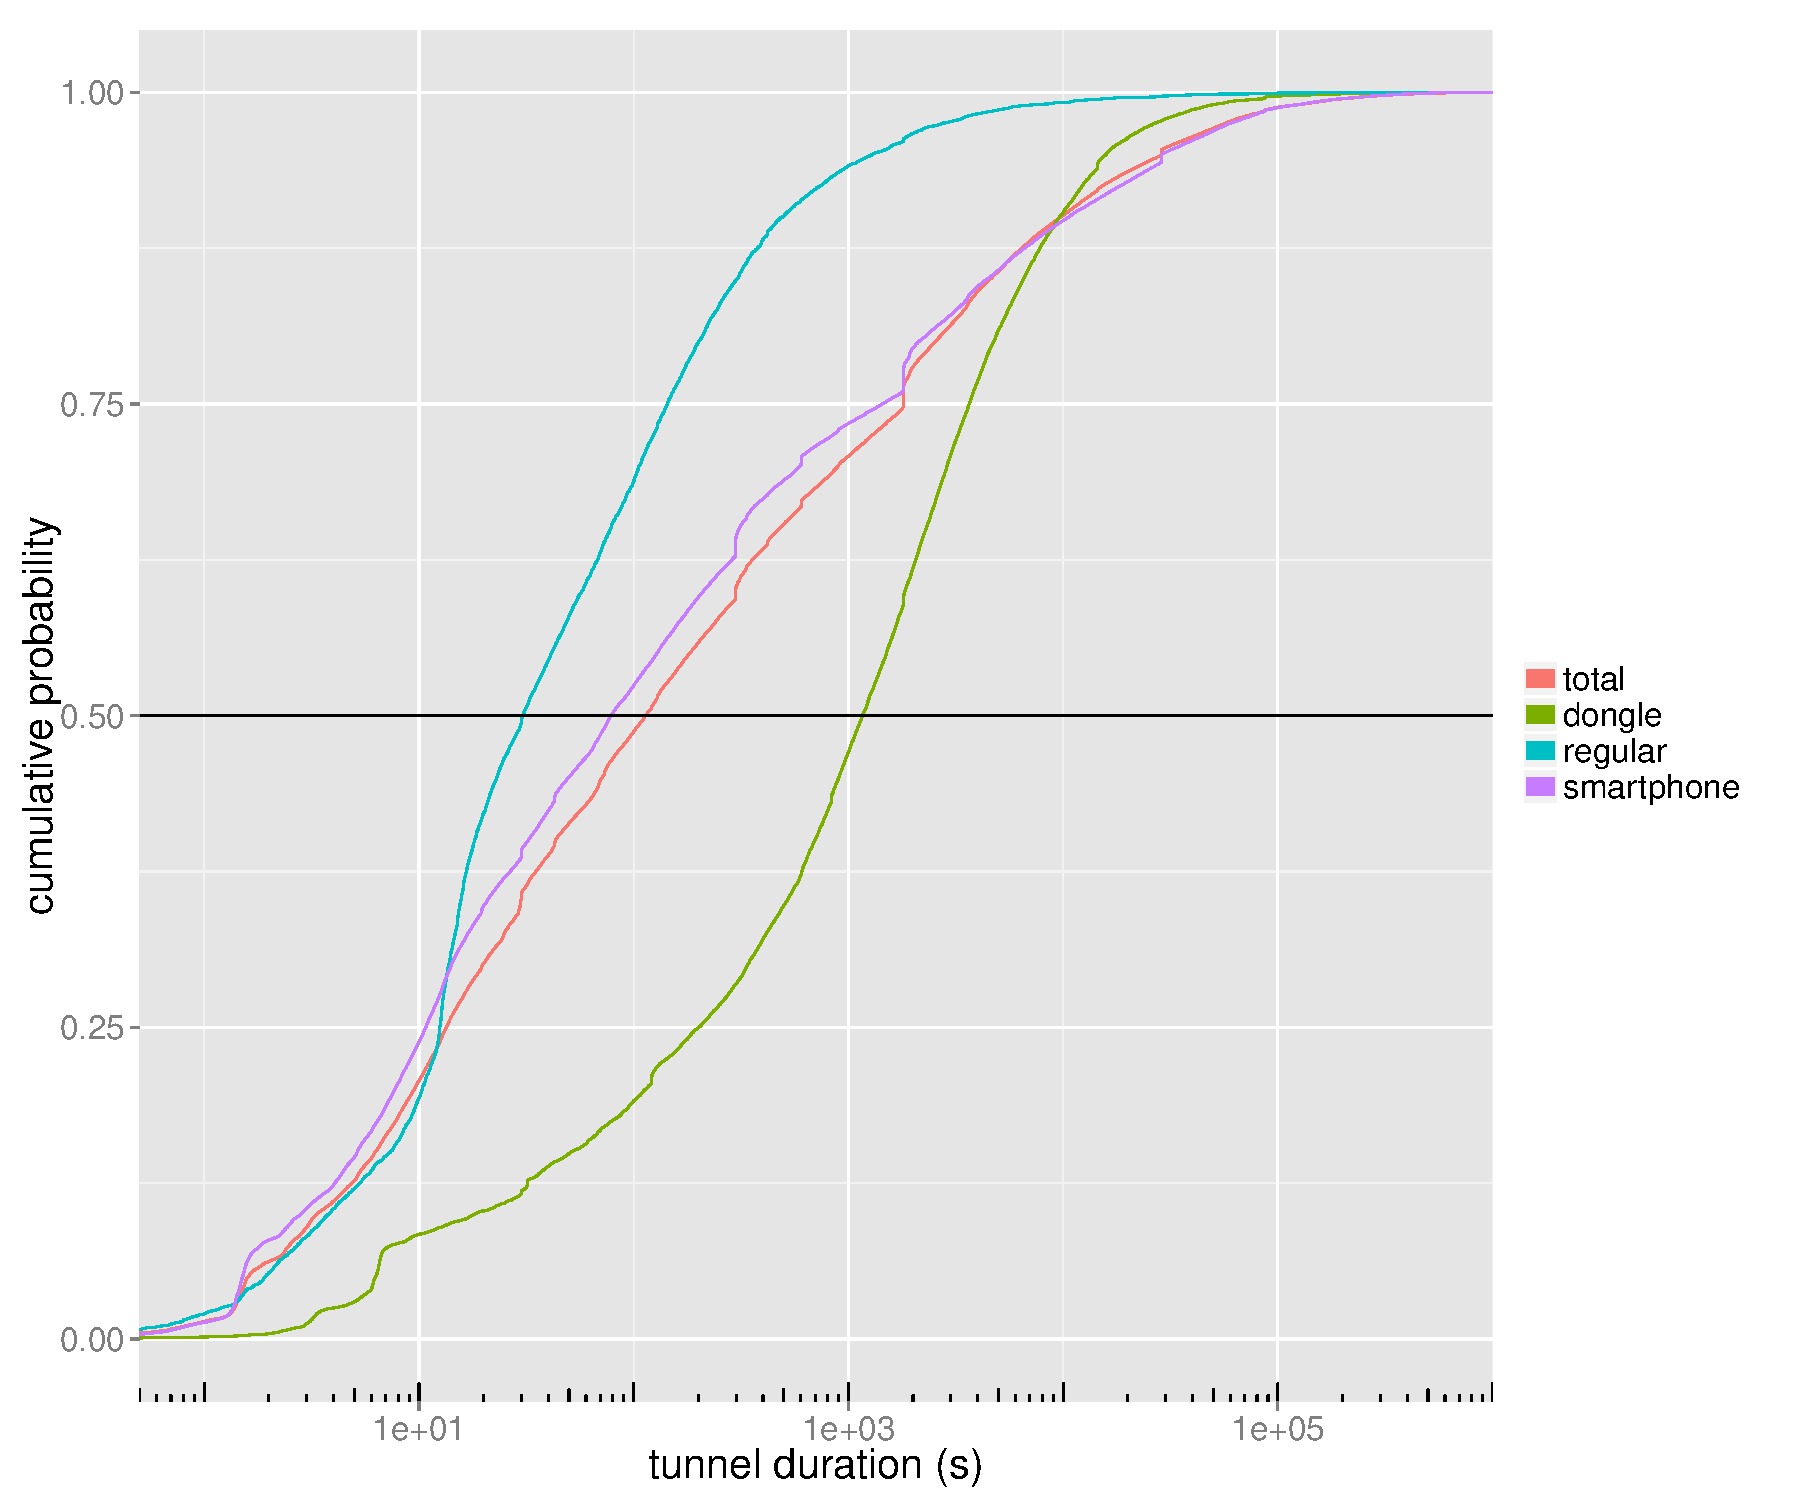
\includegraphics[width=0.9\textwidth]{images/R-tunnel-duration-device-type.pdf}
	\caption{Tunnel duration distribution, separated for \acrshort{3G} dongles, smartphones and regular phones with medians at \SI{115}{\second} (total), \SI{31}{\second} (regular), \SI{82}{\second} (smartphone), and \SI{1207}{\second} (dongle).}
\label{c4:fig:cdf-duration-device-class}
\end{figure}

Figure~\ref{c4:fig:cdf-duration-device-class} shows the \gls{ECDF} for the user tunnels and their \gls{PDP} Context durations in the dataset. In this first graph, the duration of different device classes is distinguished and put in perspective to the overall duration distribution. The devices classes here are smartphones, regular phones, and \gls{3G} dongles. It can be observed that tunnel durations range between seconds and more than one week.

The median can be clearly differentiated between device types, being much longer for \gls{3G} dongles than for mobile phones. This reflects expected user behavior very well and gives a first indicator on a possible influence of the user plane on the control plane.

Dongles are usually used with laptops to be able to work while being mobile. Dongle sessions last therefore often for extended periods longer than a few minutes up to hours. Also, this type of device is usually put into a standby mode after the period, which completely disables any mobile connections --- and therefore any associated tunnel --- instead of switching to low power radio idle modes. This is reflected in the dongle tunnel duration here as well. When compared to the other device category, dongles are more compactly centered around their median of about \SI{20}{\minute}.

A similar behavior can be observed in the regular phone distribution with values arranged tightly around the median of \SI{31}{\second}. Compared to today's smartphones, data connections on regular phones are mostly initiated explicitly by user interaction, for example through starting a browser and viewing a web page. This could also explain the comparatively low durations here.

The picture is rather different in the smartphone tunnel duration. Here, often background tasks are running over long periods of time and devices try to keep connectivity up as long as possible (while still attempting to conserve power). Overall, this could lead to the smoother distribution seen here with no clear center value.

Overall, a relatively high number of tunnels with a duration shorter than \SI{10}{\second} can also be observed. Especially the peak at about \SI{1.5}{\second} --- which is interestingly shifted to \SI{6.8}{\second} in the dongle distribution --- is of note. This is even shorter than the default values for the \gls{RRC} idle state transitions which causes the tunnel to be destroyed. It can be conjectured that these short tunnels have been explicitly removed by the \gls{UE} as no other involved state machine has timers this short.

Another distinct step at \SI{30}{\minute} in the total and smartphone distributions can be observed. As it is only present in these to categories --- and the total distribution looks to be mostly governed by smartphones --- it is reasonable to assume that the cause for this is a specific behavior observable in some aspect of smartphone related influence factors.


%%
\paragraph{Influence of the \texorpdfstring{\acrshort{os}}{OS}}

\begin{figure}[htb]
	\centering
	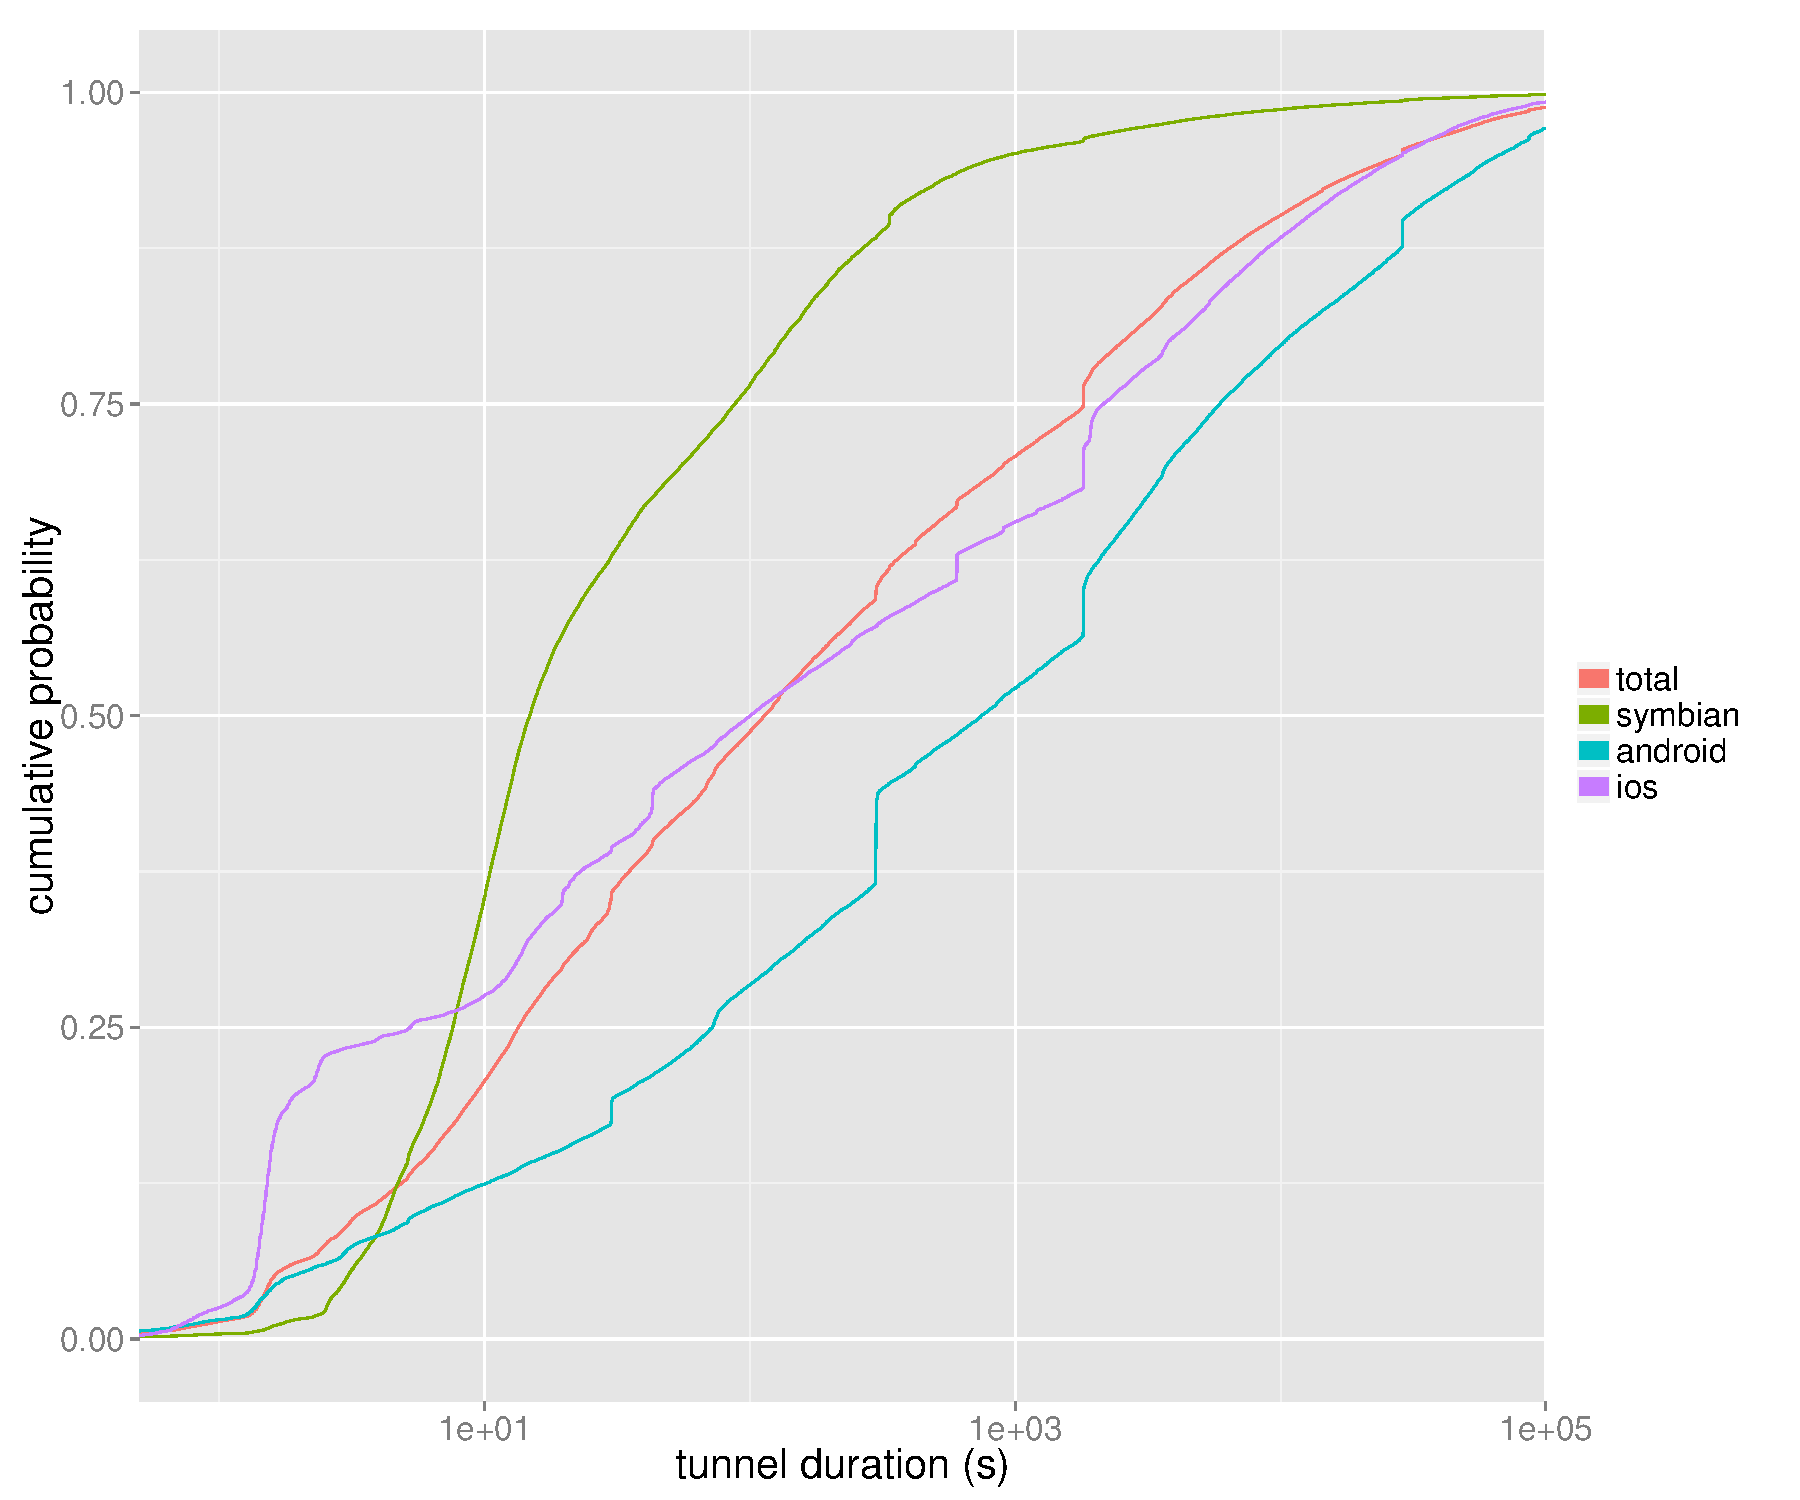
\includegraphics[width=0.9\textwidth]{images/R-tunnel-duration-operating-system.pdf}
	\caption{Tunnel duration \acrshort{CDF}, separated for select \acrshortpl{os}; Medians at \SI{115}{\second} (total), \SI{15.5}{\second} (symbian), \SI{104}{\second} (iOS), and \SI{765}{\second} (android).}
\label{c4:fig:cdf-duration-os}
\end{figure}

Next, the two phone categories are further broken down by their \gls{os}. Only the three major systems, Android, iOS, and Symbian, are identified here, the amount of other types was negligible. The smartphone category is almost exclusively represented by Android and iOS devices, while Symbian devices make up most of the regular phones but is also represented in a number of smartphone models.

Figure~\ref{c4:fig:cdf-duration-os} depicts the \gls{ECDF} of the tunnel durations of these categories in relation to the total duration distribution. They immediately exhibit a clear difference between individual \glspl{os}.

The Symbian tunnel durations are similarly distributed to the previously depicted regular phone category, albeit with an even shorter duration median of about \SI{15}{\second}. This is an indicator of the large intersection between these two groups and the explicit user traffic property attributed to regular phones.

The two smartphone-exclusive \gls{os} have remarkably similar tunnel distributions with the exception of the Android tunnel distribution shifted to much longer tunnels. This is mostly due to the larger accumulation of iOS tunnels around the previously mentioned \SI{1.5}{\second} mark. Over \SI{20}{\percent} of all tunnels established by iOS devices are shorter than \SI{2}{\second}. A possible explanation is an interaction between the described implicit background traffic happening in intervals and the efforts of iOS phones to preserve as much energy as possible. 

To this end, phones aggressively force their radio connection to the low power idle states or even completely shut off the radio immediately after transmission have ended, circumventing \gls{RRC} timers. To achieve this, iOS devices are known to implement a form of \gls{3GPP} Fast Dormancy~\cite{gsma2011fdbestpract}. It is deemed to improve device battery life, radio signaling and radio spectrum efficiency. Due the more frequent state transitions it also could cause an increase in core network tunnel management signaling, which is probably what happened in the iOS case depicted in the \gls{ECDF}.

Another set of tunnel duration accumulations are also visible in the \gls{os} distributions. Two types of steps should be distinguished here. First are accumulations that occur across multiple or all categories. This points to an influence source outside of the specific category. If the artifact is present in every distribution it is even likely that the source is a behavior of the network's state machines. The second type of accumulation is local to one or some categories, which places the root cause into the region of these categories and their related influence factors. 

In case of the \gls{os} category, additionally, peaks at \SI{30}{\second}, \SI{300}{\second}, and \SI{600}{\second} can be observed. However, whether this behavior can be attributed directly to the operating systems themselves cannot be decided just by looking at these distribution. Other factors, e.g., the device's baseband and user traffic dynamics, also play a role. 


%%
\paragraph{Influence of the Time of Day}

\begin{figure}[htb]
	\centering
	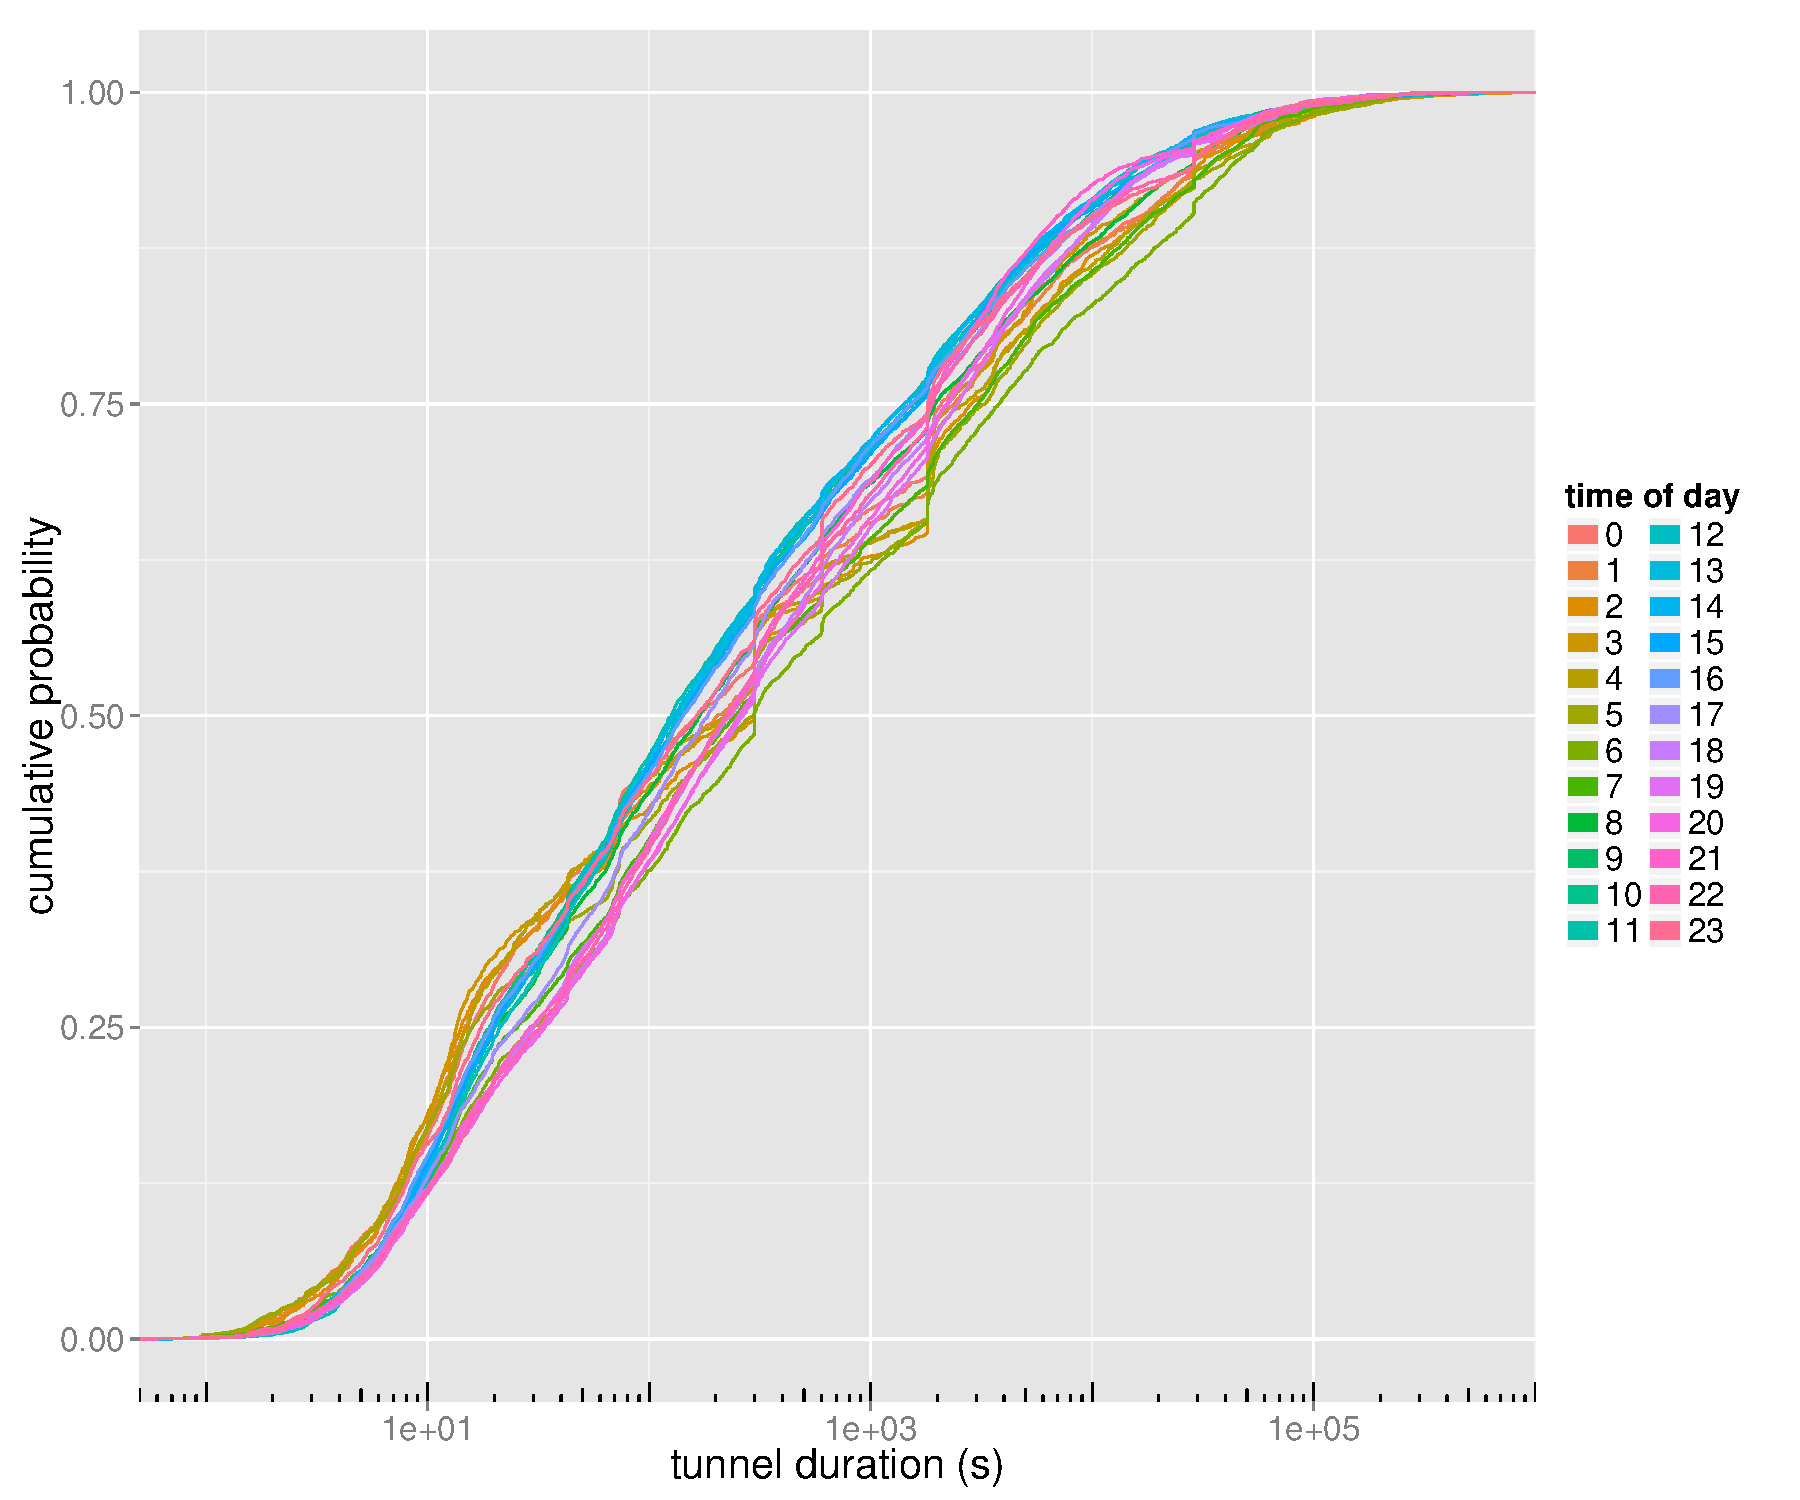
\includegraphics[width=0.9\textwidth]{images/R-duration-timeofday-ecdf.pdf}
	\caption{Tunnel duration of all active tunnels by time of day.}
\label{c4:fig:duration-timeofday-ecdf}
\end{figure}

In addition to device factors, diurnal effects could also play a role in the duration of tunnels. Figure~\ref{c4:fig:duration-timeofday-ecdf} depicts $24$ individual \glspl{ECDF} of the tunnel duration for each hour of a day. While no clear distinctions are visible, there is a trendto shorter tunnels in the early morning hours. The early afternoon hours tend to produce tunnels more centered around the middle duration range. Even longer tunnels should be treated with reservation, as they exceed the length of their assigned time slot in the \gls{ECDF} and span a larger time frame. Only the tunnel creation point is guaranteed to be in the slot.


%%
\paragraph{Influence of Other Factors}

Due to the nature of the trace dataset at hand many other influence factors are hard or outright impossible to distinguish. Some factors are unknown from the \gls{CN} perspective, as the mentioned device baseband, while others have not been recorded in the trace.

For example, it would theoretically be possible to investigate the influence of the \gls{RAT} as it is an \gls{IE} in the \gls{gtp} messages and also recorded in the trace. The radio access parts of \gls{GSM} and \gls{UMTS} are completely different --- including the \gls{RRC} state machines which were depicted in Figure~\ref{c4:fig:mmstatemodel} --- and therefore could also differ in their control plane load impact on the core. However, the \gls{RAT} \gls{IE} is optional and only set in less than \SI{1}{\percent} of the available records. As the radio access can change even during an existing tunnel --- in which case the \gls{GGSN} receives a \gls{gtp} update request informing the node about the change --- a complete picture without gaps would be required to do any investigation on this.


%%
\paragraph{Influence Strength of the Categories}

\begin{figure}[htb]
	\centering
	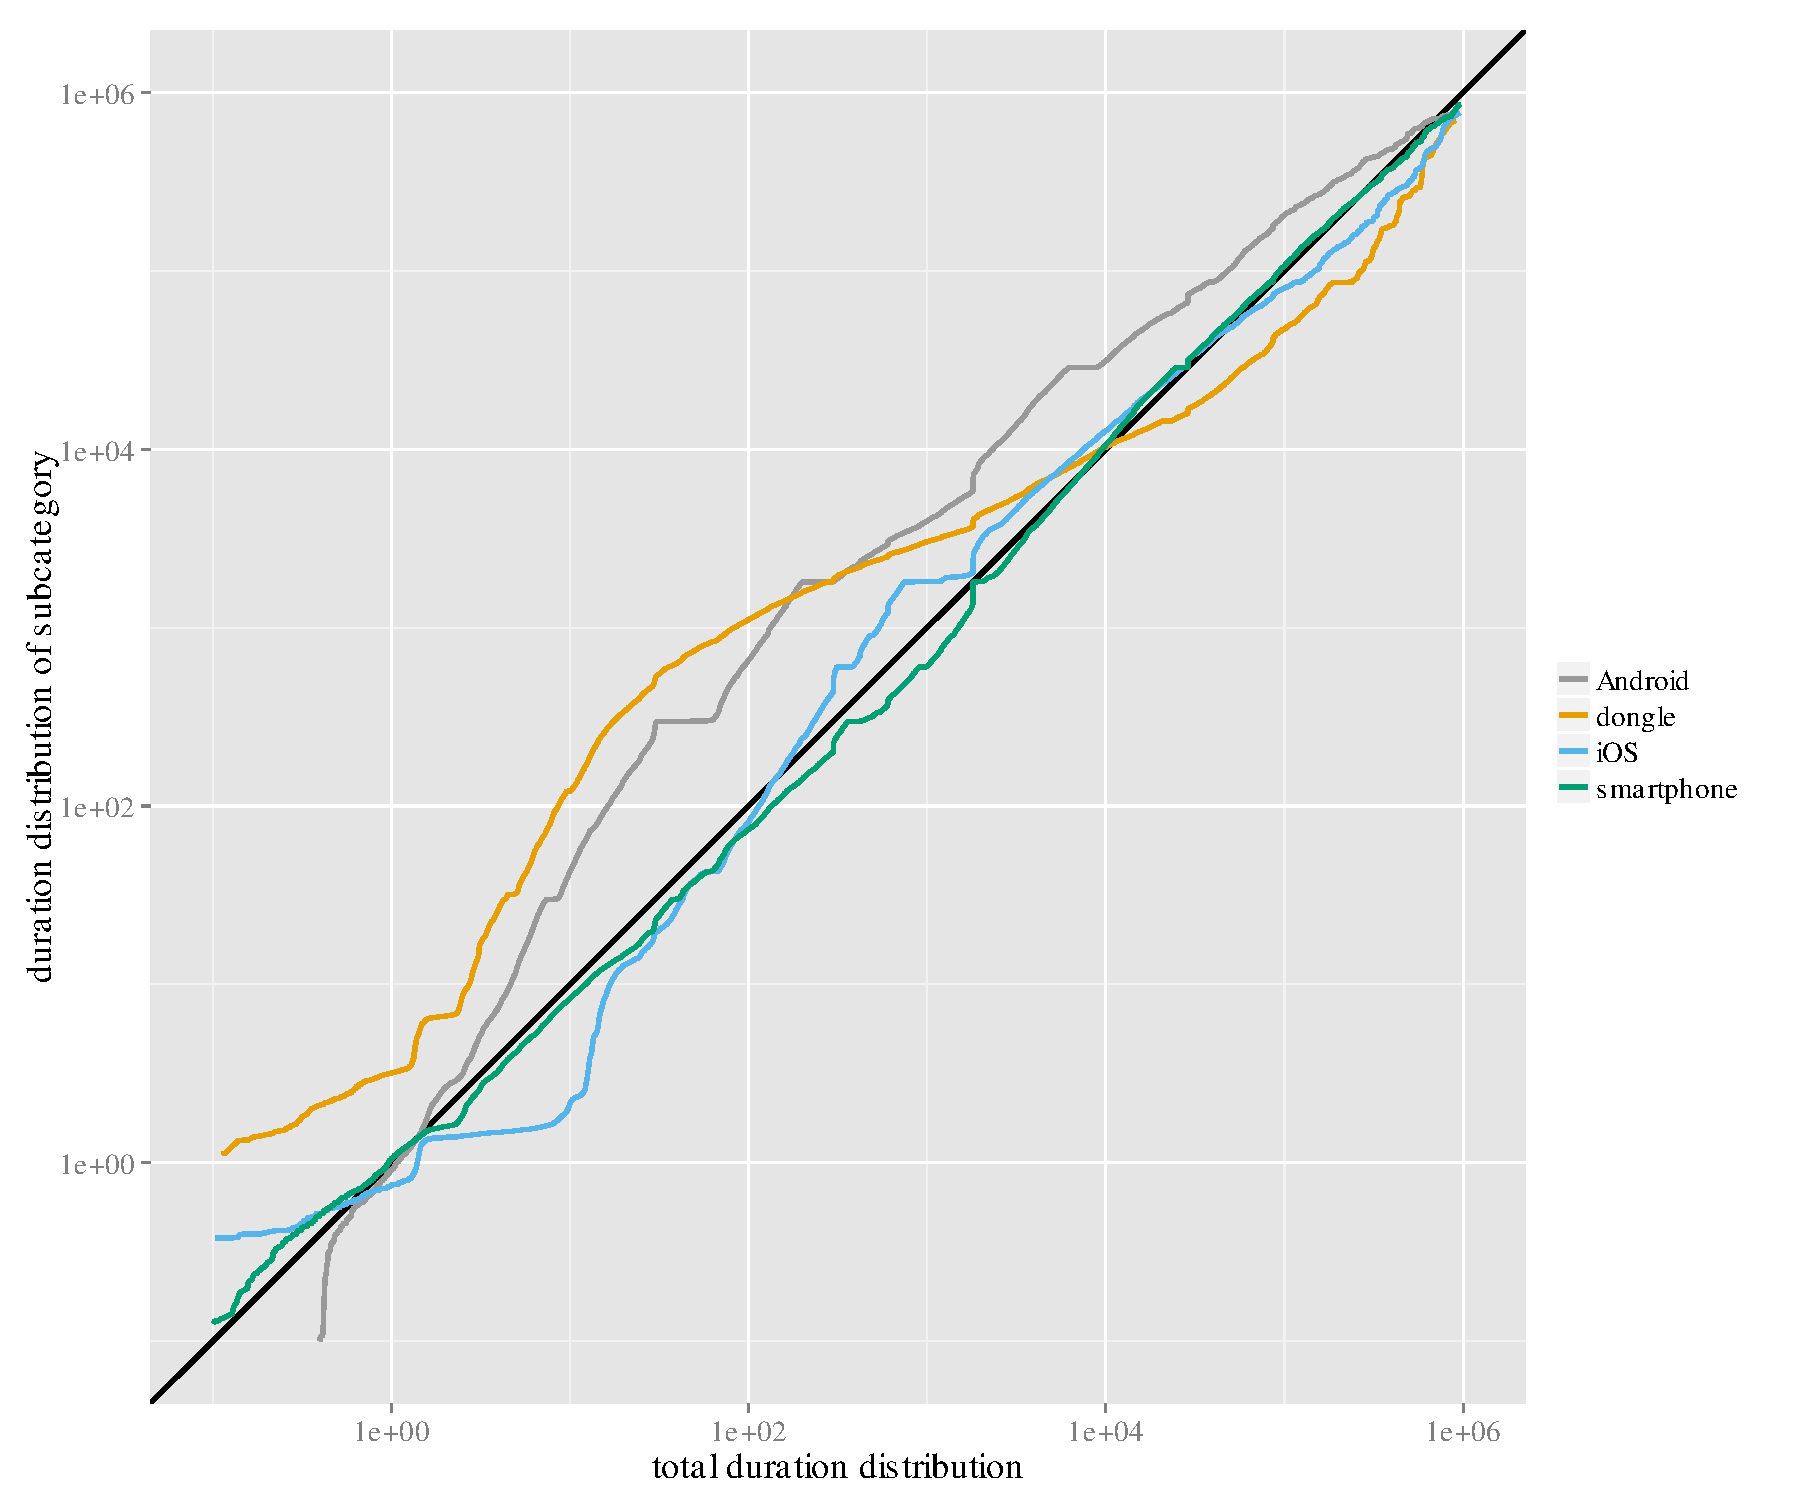
\includegraphics[width=0.9\textwidth]{images/R-duration-qq-category-comparison.pdf}
	\caption{Q-Q Plots of the tunnel duration distributions in comparison to device classification categories.}
\label{c4:fig:qq-plots}
\end{figure}


To ascertain which of the investigated device categories influences the total duration distribution most, Q-Q plots are created and investigated. It is conjectured that the amount of influence on the duration distribution is correlated to the influence on the control plane load. In theory, if both durations follow the same distribution, one expects a straight diagonal $y=x$ line through the origin. A steeper incline indicates more compact regions in the distribution plotted on the $x$ axis and vice versa.

The Q-Q plots in Figure~\ref{c4:fig:qq-plots} compare the total tunnel duration distribution to the duration distribution of the dongle, smartphone, Android, and iOS classification cateogries. It can be observed that the smartphone duration distribution is distributed almost equally to the total except for minor variations. However, the \gls{3G} dongle tunnel durations follow a very different distribution. Their effect on the total duration distribution seems to be negligible despite the  large amount of traffic they are causing. This is also a first indicator that smartphones might have a larger impact on signaling than other device types.

Looking closer at the smartphone category, Q-Q plots of the two major \glspl{os} are investigated. With the exception of the large below \SI{2}{\second} peak in the lower tail of the distribution, iOS device tunnel durations are very similar to the overall tunnel duration distribution. The same can not be said about the Android distribution, which deviates somewhat in the distribution's center but is similar to the total distribution in the upper tail. Even devices with just a different \glspl{os} seem to strongly differ in their influence on duration distribution and therefore on signaling.

\begin{figure}[htb]
	\centering
	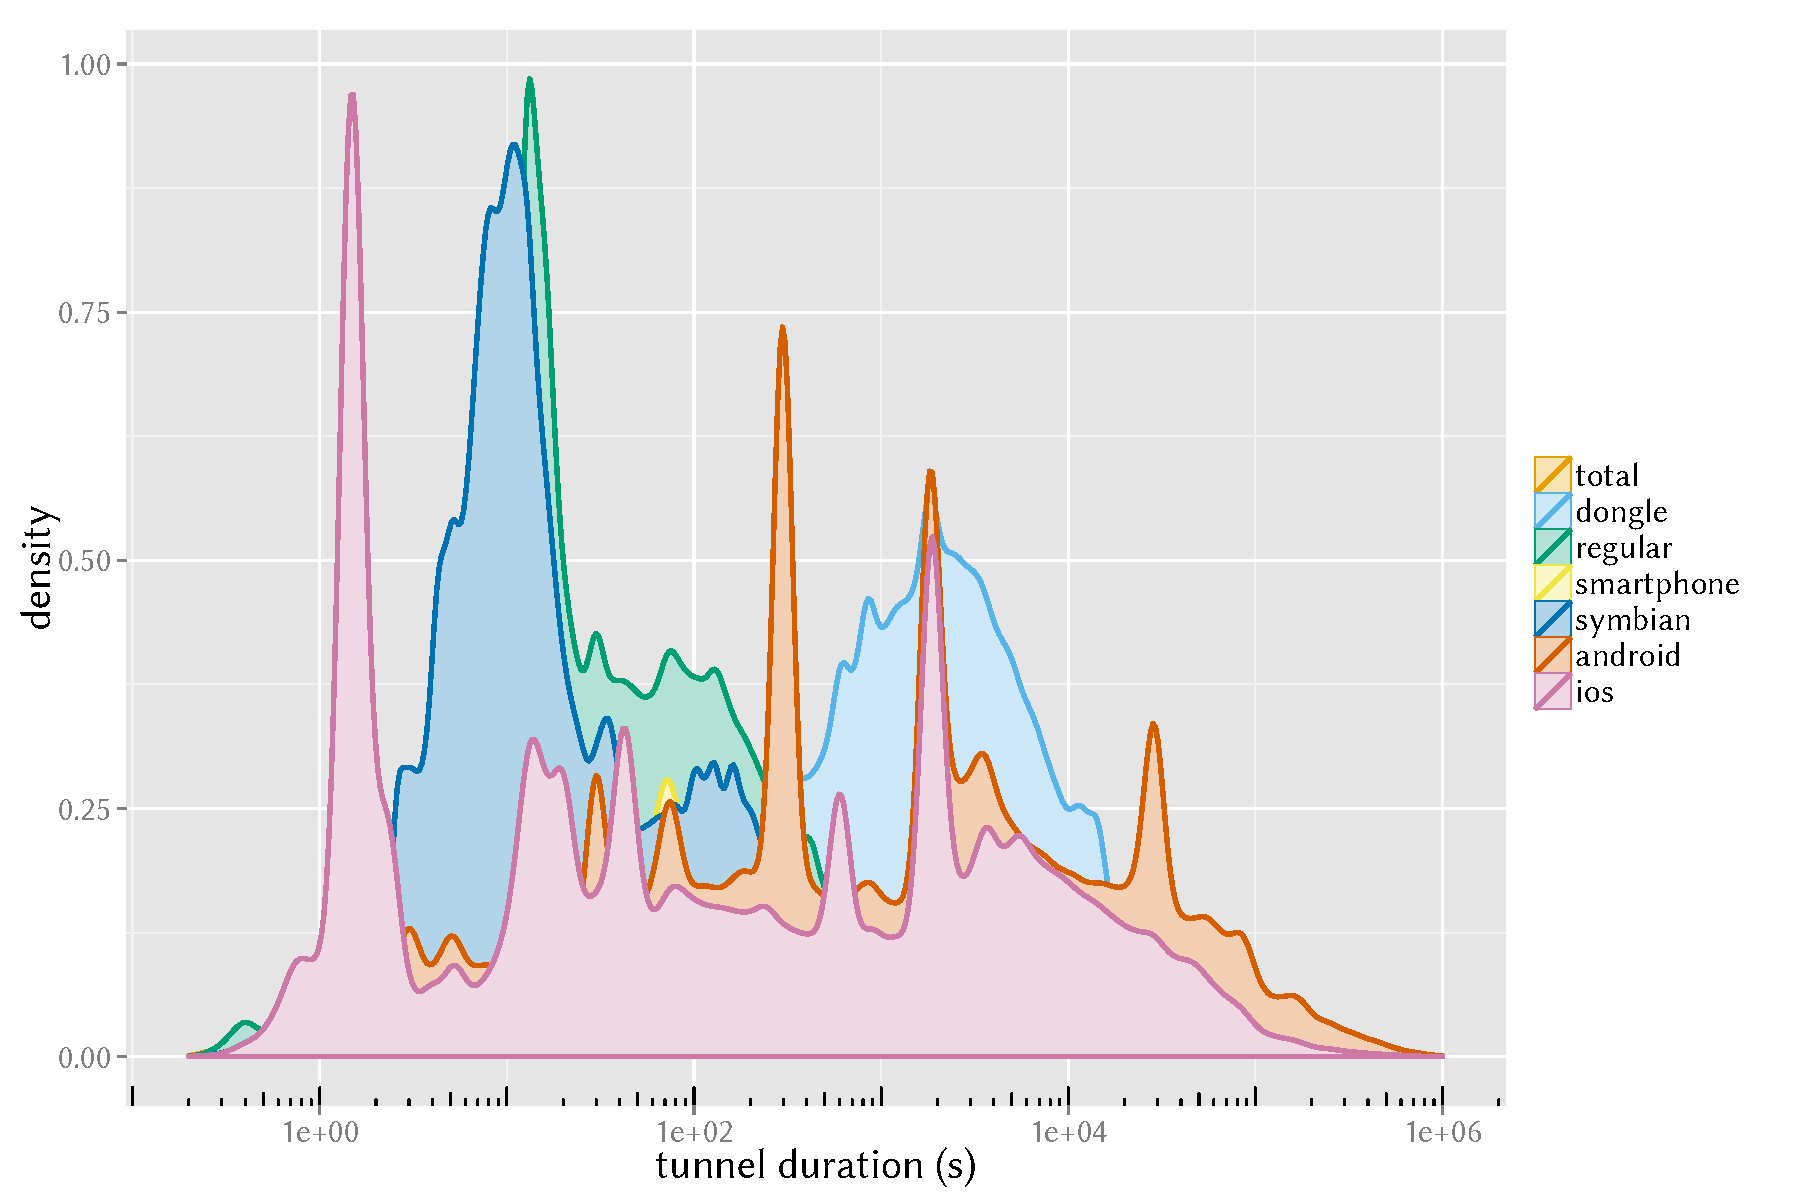
\includegraphics[width=0.9\textwidth]{images/R-duration-classification-density.pdf}
	\caption{Logscale density plot of the tunnel duration with all classifications.}
\label{c4:fig:durations-density}
\end{figure}


Figure~\ref{c4:fig:durations-density} attempts to depict where in their distributions the investigated device categories show the most impact on the total distribution. The plot shows the density of all previously investigated device influence categories.

It is evident that the durations are not evenly distributed, but rather follow sharp spikes. One of largest spike across all categories is the one at a duration of \SI{30}{\minute}, with about \SI{1.8}{\percent} of all tunnels in the network falling into that region. Since this spike happens across all device types, it makes a rather strong case for being induced by the network. On the other hand, the bulk of tunnel durations in the short-to-medium range does not seem to be governed by the two major smartphone operation systems but by other devices in the network, which do not show major spikes in other bins.

Besides the long-tailed behavior in the upper tail of the tunnel durations another slight accumulation effect, repeating itself every \SIrange{6}{7}{\day}, is present in the upper tail. This phenomenon is as yet of unknown origin and does not coincide with any known timers of the \gls{3G} mobile network.

The investigation of this data leads to the conclusion that the planning and dimensioning of the control plane needs to watch the behavior of smartphones more carefully than that device types.


%%%%%%%%%%%%%%%%%%%%%%%%%%%%%%%%%%%%%%%%%%%%%%%%%%%%%%%%%%%%%%%%%%%%%%%%%%%%%%%
\subsubsection{\texorpdfstring{\acrshort{gtp}}{GTP} Tunnel Arrivals}

The duration of \gls{gtp} tunnels is but one aspect of influence on control plane load. The arrival process of these tunnels is also interesting in itself. Specifically, this mean the arrival of tunnel requests, i.e.\gls{gtp} create requests, at the \gls{GGSN}. 

An arrival process can be described in two distinct ways. First by the number of arrivals in a given time interval. Second, by the \gls{IAT}, the time between two consecutive tunnel arrivals. Depending on the choice one has to deal with either a discrete or a continuous distribution.

Here, the tunnel arrival process is investigated with both approaches. This also adds to the foundation of the load model constructed in the next chapter. Note, that the notion of classifying arrivals into influence categories based on device specifics is omitted here. An investigation of this process can not be realistically be conducted categorized and still relate to the total system load.

\begin{figure}[htb]
	\centering
	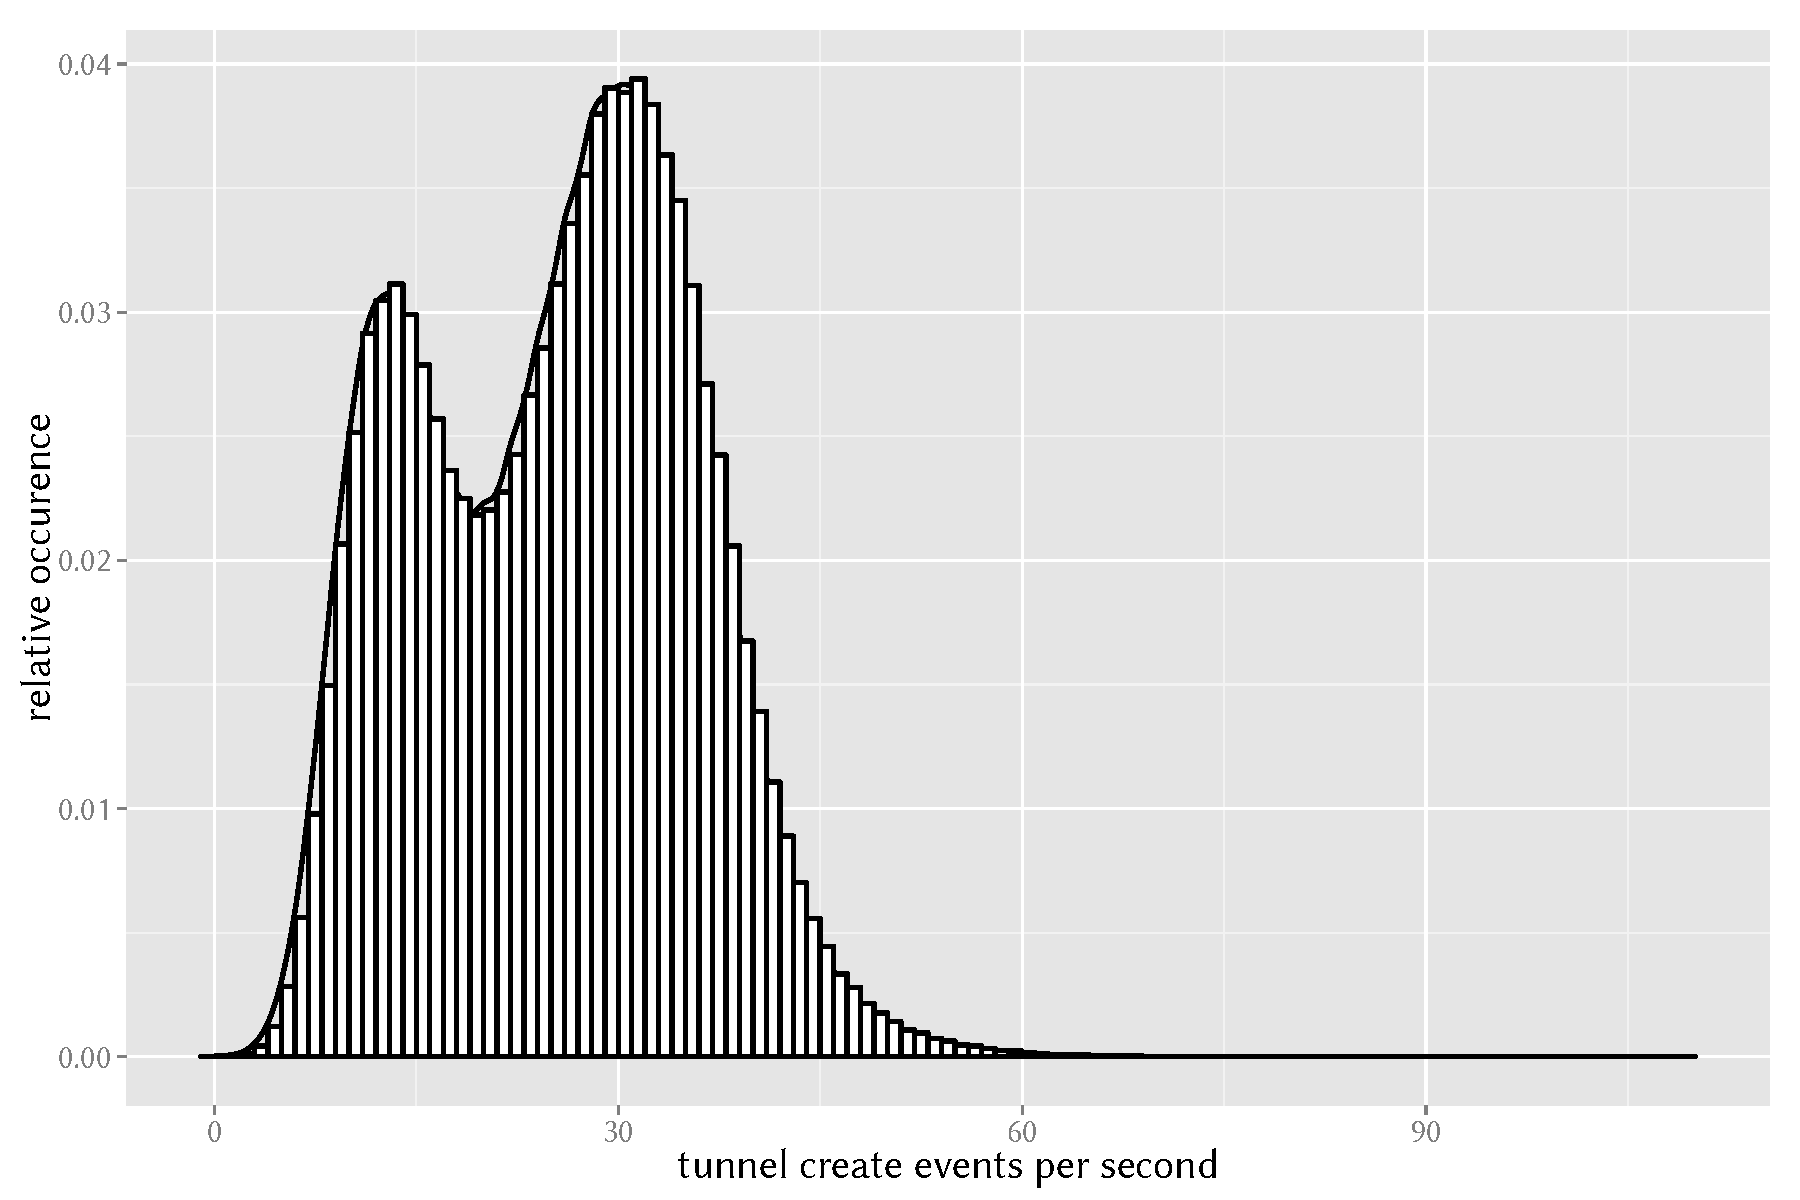
\includegraphics[width=0.9\textwidth]{images/R-create-frequency.pdf}
	\caption{Tunnel arrivals histogram overlaid with a density plot.}
\label{c4:fig:freq-arrivals}
\end{figure}

Figure~\ref{c4:fig:freq-arrivals} depicts a histogram the number of tunnel arrivals per second during the whole trace duration period. Of note is the clear bimodal nature with one peak around twelve and the other in the low thirties. While the distribution is rather compact around these two peaks, there are some clear outliers peaking at $107$ arrivals per second. If the hypothesis of the correlation between signaling load and number of arrivals holds, it can be assumed that load is not constant but rather switches between two modes with some periods of very high load induced by an increased number of arrivals.

\begin{figure}[htb]
	\centering
	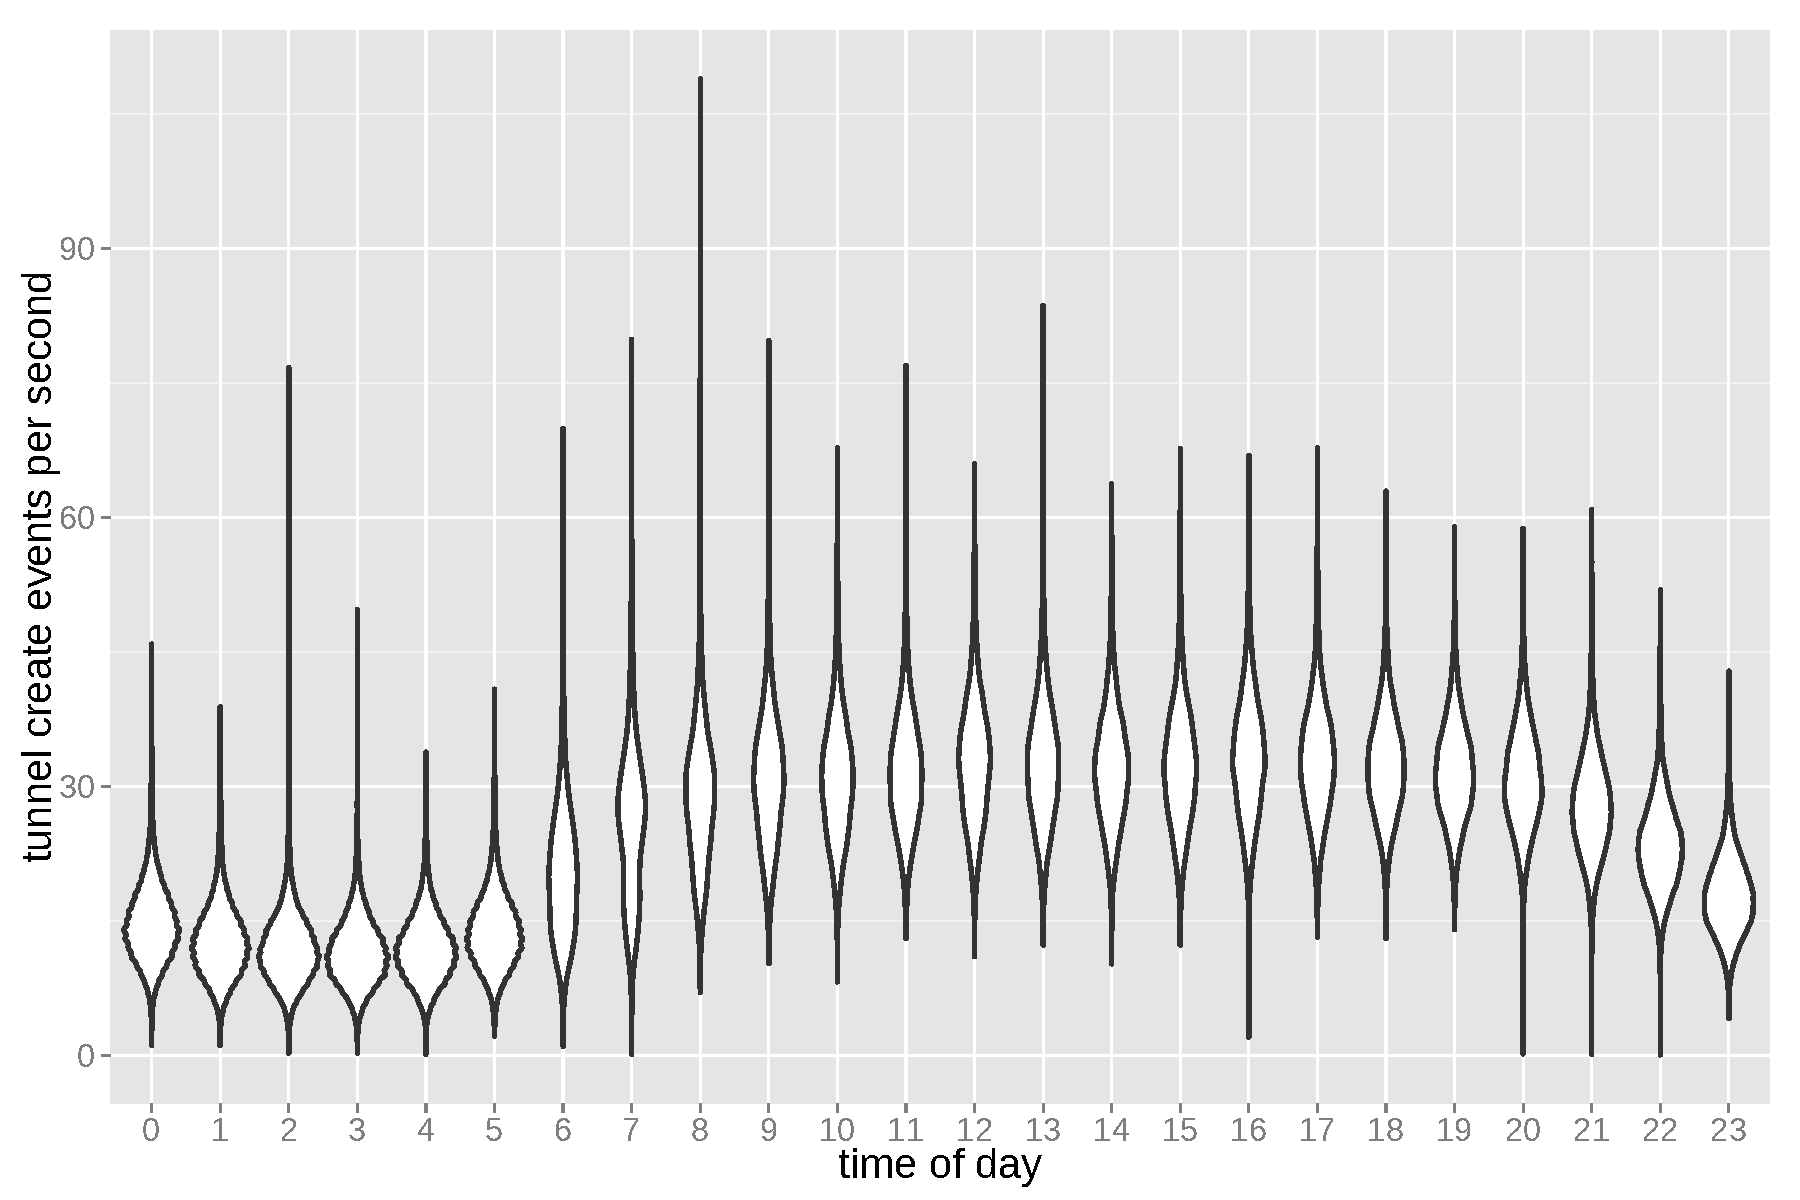
\includegraphics[width=0.9\textwidth]{images/R-createspersecond-1h-violin.pdf}
	\caption{Violin plot of tunnel arrivals in one second per time of day.}
\label{c4:fig:freq-arrivals-per-second-violin}
\end{figure}

A reasonable cause for the occurrence of these two modes can be found in the diurnal arrival patterns. Figure~\ref{c4:fig:freq-arrivals-per-second-violin} contains a violin plot of the tunnel arrivals. This type of plot is similar to a box plot but additionally shows the density of the individual items on the vertical axis. Here the arrivals are broken down to hourly slots. 

The nocturnal plateau of arrivals between midnight and \formattime{5}{0}{0} and the longer daytime plateau between \formattime{8}{0}{0} and \formattime{19}{0}{0} match the two modes found in the histogram. In between are short transition phases. The density of the arrivals during daytime indicates a spread of the number of arrivals over a larger range. This could be an indication of load fluctuations in the system.

\begin{figure}[htb]
	\centering
	\begin{subfigure}[b]{0.5\textwidth}    
		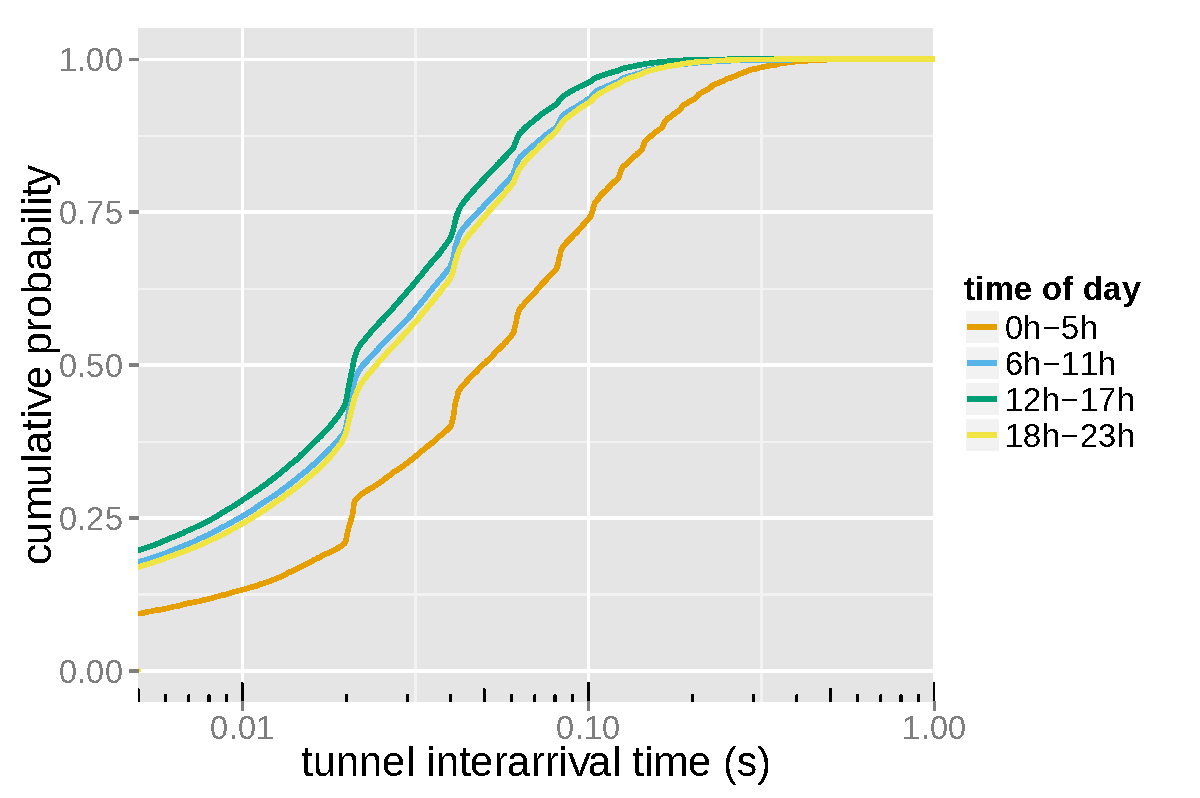
\includegraphics[width=\textwidth]{images/R-IAT-successful-2h-ecdfs.pdf}
		\caption{All tunnel requests.}
		\label{c4:fig:IAT-ecdf-2h-successful}
	\end{subfigure}%
	~
		\begin{subfigure}[b]{0.5\textwidth}
		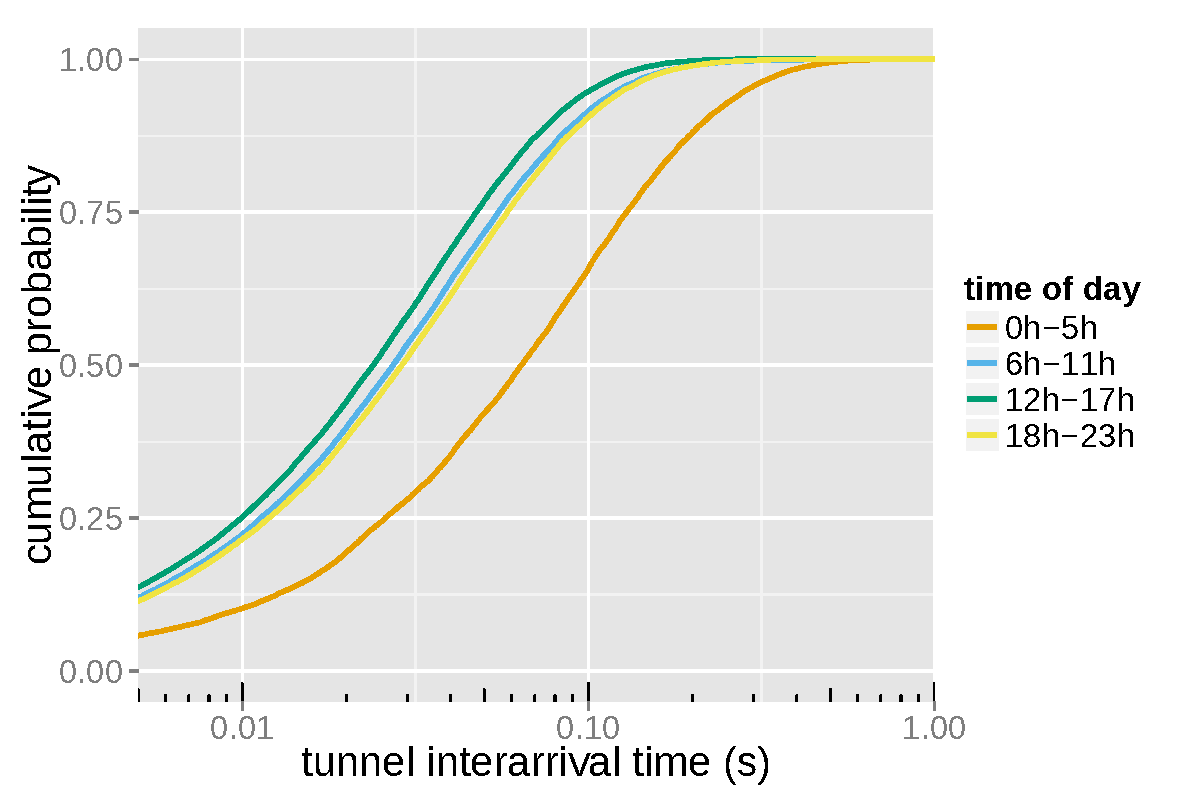
\includegraphics[width=\textwidth]{images/R-IAT-fromflows-ecdfs-2h.pdf}
		\caption{Only tunnels with data flows.}
		\label{c4:fig:IAT-ecdf-2h-active}
	\end{subfigure}

	\begin{subfigure}[b]{0.5\textwidth}
		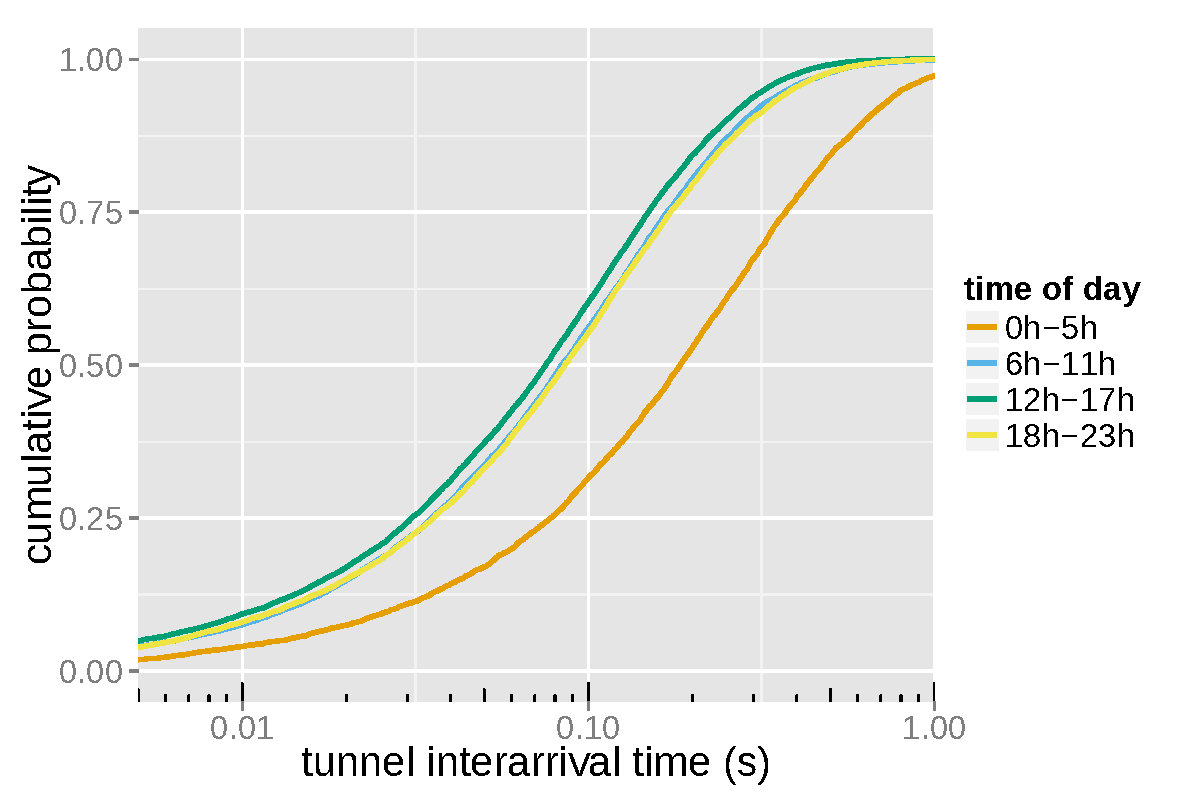
\includegraphics[width=\textwidth]{images/R-IAT-fromflows-gprs-ecdfs-2h.pdf}
		\caption{Tunnels with data flows initiated in \gls{GPRS}.}
		\label{c4:fig:IAT-ecdf-2h-active-gprs}
	\end{subfigure}%
	~
	\begin{subfigure}[b]{0.5\textwidth}
		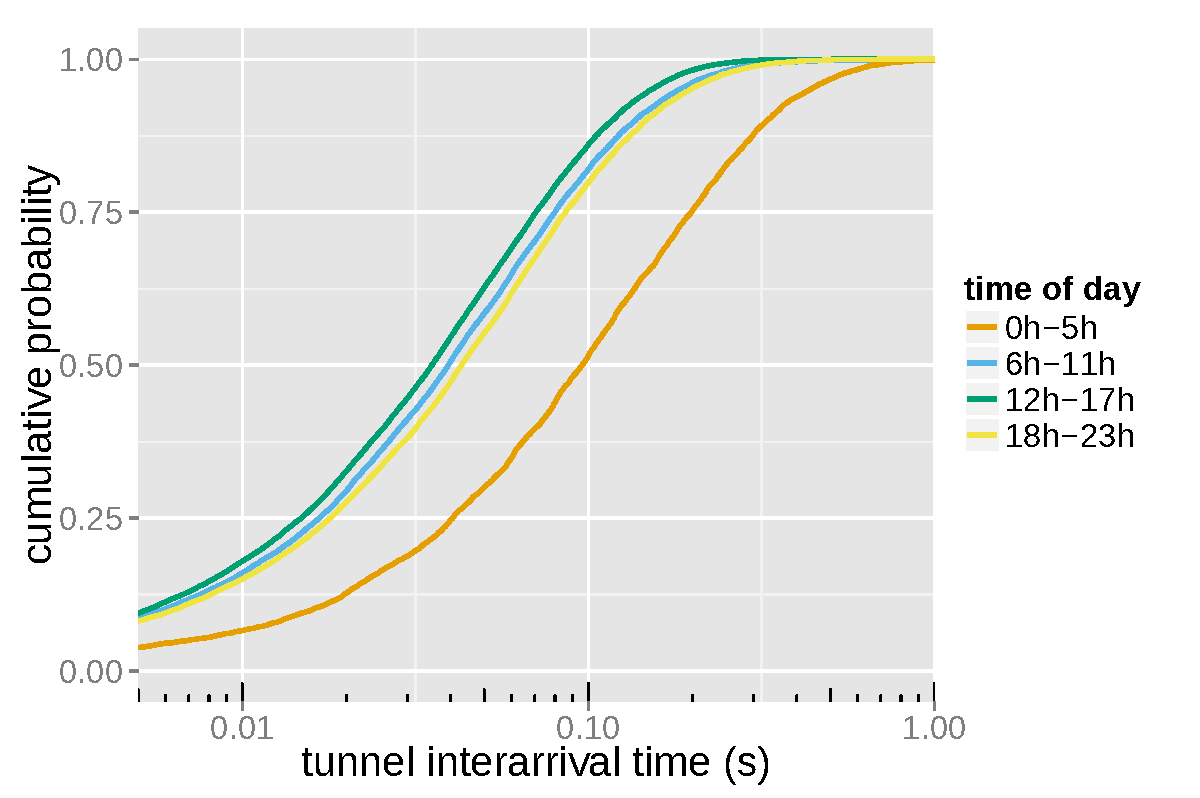
\includegraphics[width=\textwidth]{images/R-IAT-fromflows-umts-ecdfs-2h.pdf}
		\caption{Tunnels with data flows initiated in \gls{UMTS}.}
		\label{c4:fig:IAT-ecdf-2h-active-umts}
	\end{subfigure}
	\caption{\acrshortpl{ECDF} of the tunnel \acrshort{IAT} in seconds by time of day.}
\label{c4:fig:IAT-ecdf-2h}
\end{figure}

Complementing the arrival rate evaluation is the investigation of the tunnel \gls{IAT}. This metric is more sensitive to short time fluctuations of arrivals and more suited to describe the arrival process for use in the proposed load model.

The overall picture of all arrivals is given in the \gls{ECDF} of Figure~\ref{c4:fig:IAT-ecdf-2h-successful}, again broken down by time of day. Obviously the the same previously observed diurnal load oscillation can again be perceived. The median \glspl{IAT} fall in the range of \SI{20}{\milli\second} and \SI{60}{\milli\second}, enveloped by the \formattime{16}{0}{0} and \formattime{2}{0}{0}distributions on with the lowest and highest \gls{IAT} respectively. Additionally, tunnel arrivals are occurring at an increased frequency with an interval of multiples of \SI{20}{\milli\second}, which generates these wave-like steps in the \gls{ECDF} plot. As this is happening very regularly at every time of the day, a source inside the mobile network is indicated.

A hypothesis as to the origin of this effect is the value of the \gls{TTI}. This property determines the duration of a mobile network's radio transmission slot. In \gls{3GPP} standards up to \gls{UMTS} the default value of the \gls{TTI} is either \SI{10}{\milli\second} or \SI{20}{\milli\second}, newer versions of the specification set the value to \SI{2}{\milli\second} (in \gls{HSPA}) or even \SI{1}{\milli\second} (for \gls{LTE}). The absolute time of every transmission slot is also synchronized across every base station in the whole mobile network, which makes the \gls{TTI} noticeable even when not measuring directly at the radio link. 

The observed step-width of \SI{20}{\milli\second} therefore indicates that the tunnel establishment signaling procedure includes at least one trip from the mobile device over the radio interface. This makes sense, as the tunnel is typically created during the \gls{GPRS} Attach procedure, which is indeed initiated at the user's device. Unfortunately, this gives the arrival process batch properties. As a result the load at the \gls{GGSN} increases momentarily when a batch arrives. The \gls{GGSN} would then need to process more requests simultaneously than if the arrivals followed a smooth stochastic distribution.

This effect becomes more peculiar when the tunnel arrivals are further broken down. Figure~\ref{c4:fig:IAT-ecdf-2h-active} only displays arrivals of tunnels that actually transported user traffic during their lifetime. Here, the influence of the effect is visually unnoticeable. This could be attributed to the fact that most active data connections during the time of the trace recording were already using almost exclusively \gls{HSPA} or better, which sees the much lower \gls{TTI}. Only older, regular phones establish plain \gls{UMTS} connections and often do not even use it.

The discrimination of the \gls{IAT} distribution by \gls{RAT} that was used during the creation of the tunnel reveals no further information. Due to the much lower number of connections the \gls{GPRS} distributions are shifted to much higher intervals than the \gls{UMTS} specific distributions.


%%%%%%%%%%%%%%%%%%%%%%%%%%%%%%%%%%%%%%%%%%%%%%%%%%%%%%%%%%%%%%%%%%%%%%%%%%%%%%%
\subsection{\texorpdfstring{\acrshort{gtp}}{GTP} Tunnel Message Processing Time}

Finally, the \gls{GGSN}'s processing time of \gls{gtp} tunnel management messages is investigated. Potentially, this can be a direct measure of the load at the node. In times of higher load one would expect a higher processing time of signaling messages.

From the network trace the processing time can be calculated by two timestamps in each record.
As the trace is recorded at the Gn interface these timestamps represent the points in time the \gls{gtp} signaling request and subsequent response pass on the link to and from the the \gls{GGSN}. Therefore, they can also be interpreted as the start and finish of the involved processing at the \gls{GGSN}.

Generally, the processing time of all three message types --- i.e., creates, deletes and updates --- could be calculated. It would be of special interest to know if the setup time of tunnels is influenced by anything, as this is one of the \gls{GGSN}'s most time-sensitive jobs and can impact the time a user has to wait before being able to actually transfer data. Unfortunately, due to unrecoverable issues with the recording of the dataset, the timestamps for both the create and delete messages records were completely unreliable and did not allow for an investigation of the processing time. 

Only \gls{gtp} update messages were unaffected and gave the opportunity for further investigation. The trace contains roughly two orders of magnitude more update messages than either creates or deletes, spread out almost evenly over the whole observation period. Therefore, a node load investigation should still be possible with just the updates messages.

\begin{figure}[htb]
	\centering
	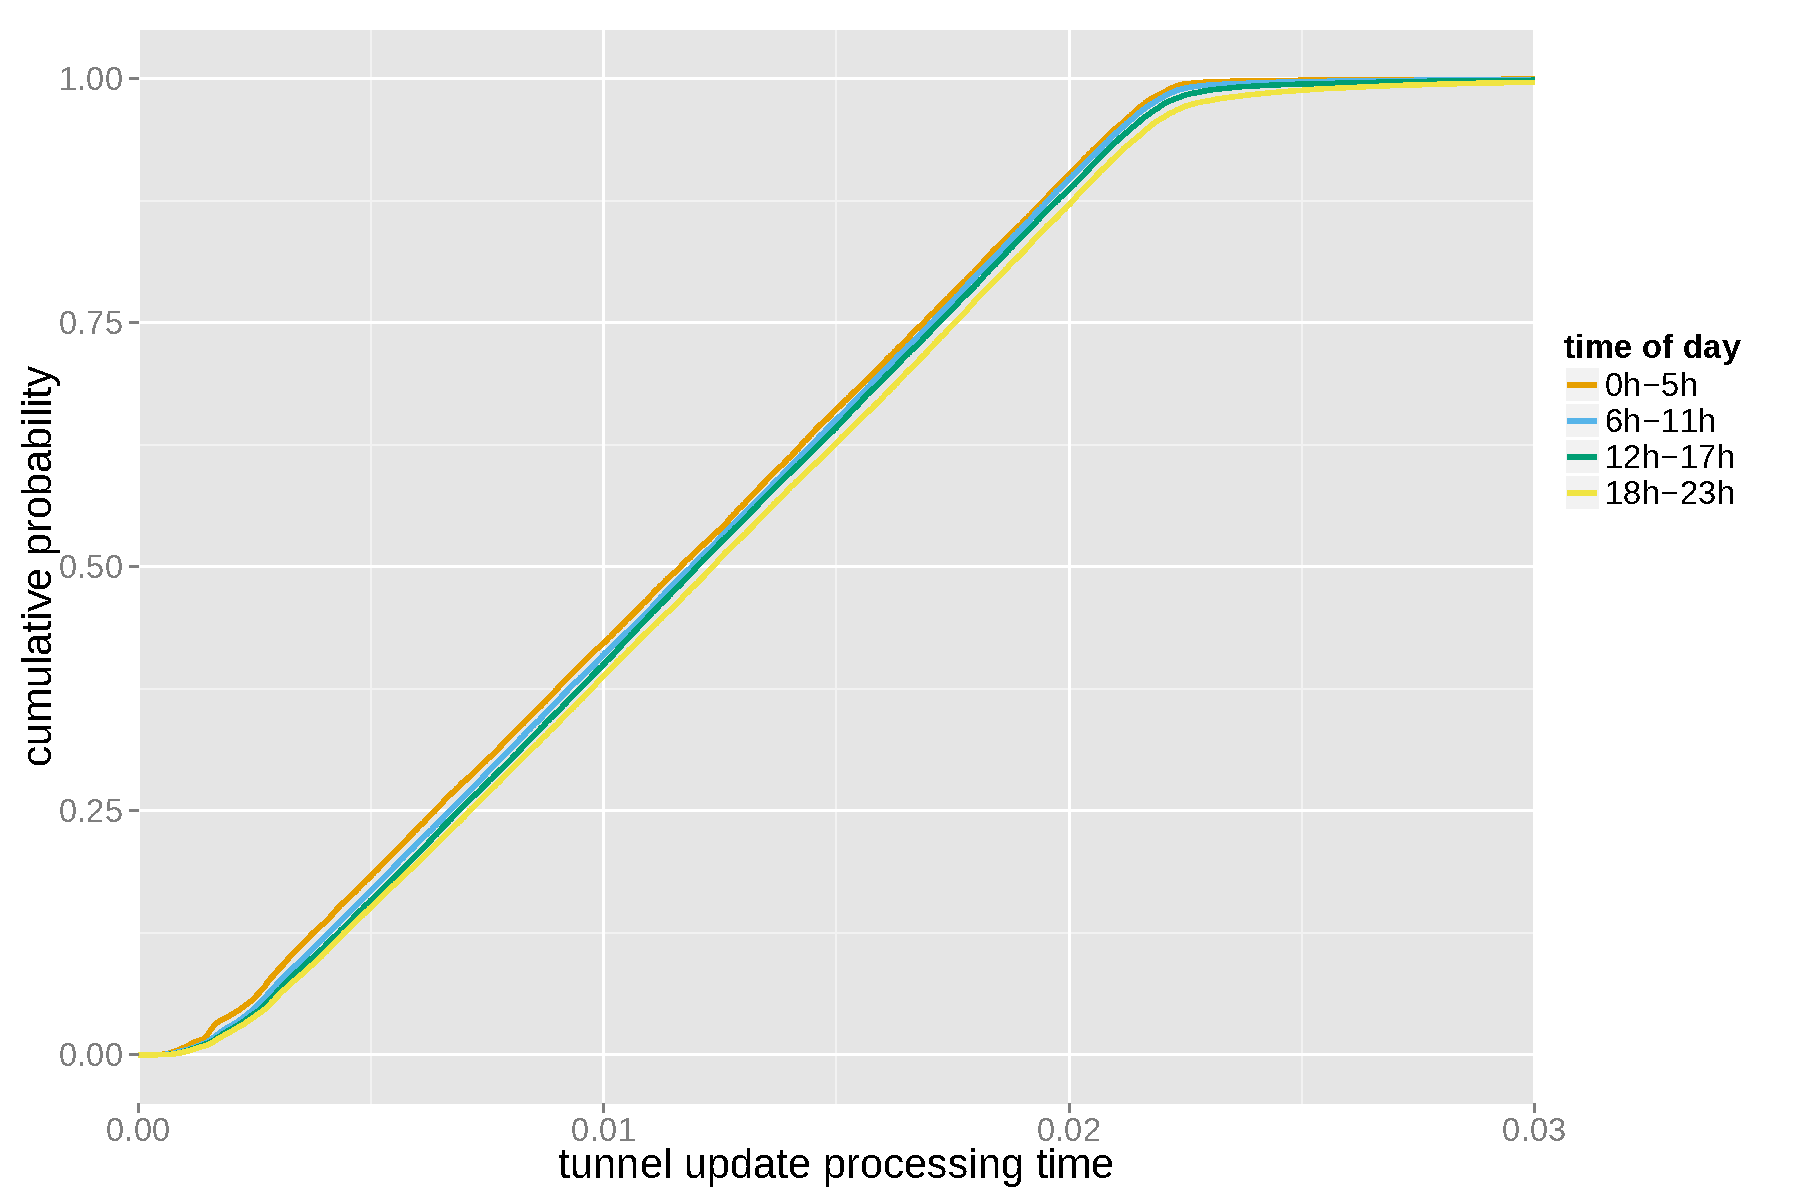
\includegraphics[width=0.9\textwidth]{images/R-update-time-cdfs.pdf}
	\caption{\acrshortpl{ECDF} of the time in seconds it takes a \acrshort{GGSN} to process a \acrshort{gtp} update event, separately plotted for four time slots each day.}
	\label{c4:fig:update-time}
\end{figure}

Figure~\ref{c4:fig:update-time} depicts a band of \glspl{ECDF} for the processing time of update messages by time of day. The processing time distribution almost perfectly follows a continuous uniform distribution between \SI{2}{\milli\second} and \SI{22}{\milli\second}. Only the upper end displays a slight long-tail behavior. The impact of the time of day is very slim with slightly higher processing times during the evening, the same time frame which also experienced an elevated arrival rate.

The occurrence of a continuous uniform distribution is rather unexpected as these do not usually occur in computing processes. According to the central limit theorem one would rather expect to see a normal distribution influenced by, e.g., process scheduling or other queuing artifacts. The source of this effect is still unknown and the current dataset does not allow for a more thorough investigation. Still, the fact that a higher update processing time coincides with an increase in the arrival rate points to an influence of tunnel messaging on the load of a \gls{GGSN}.



%%%%%%%%%%%%%%%%%%%%%%%%%%%%%%%%%%%%%%%%%%%%%%%%%%%%%%%%%%%%%%%%%%%%%%%%%%%%%%%
\subsection{Statistical Evaluation and Data Fitting}
\label{c4:sec:statistical_evaluation}

The uncovered empirical distributions for both the tunnel duration and the tunnel \gls{IAT} are now to be matched against theoretical probability distributions. Therefore, a univariate distribution fit to the experimental data was conducted. Having a concise representation for the empirical data will help in creating a model of the core network, which is the task conducted in the sections following after this.


%%
\paragraph{\gls{IAT} Fitting}

\begin{figure}[htb]
	\centering
	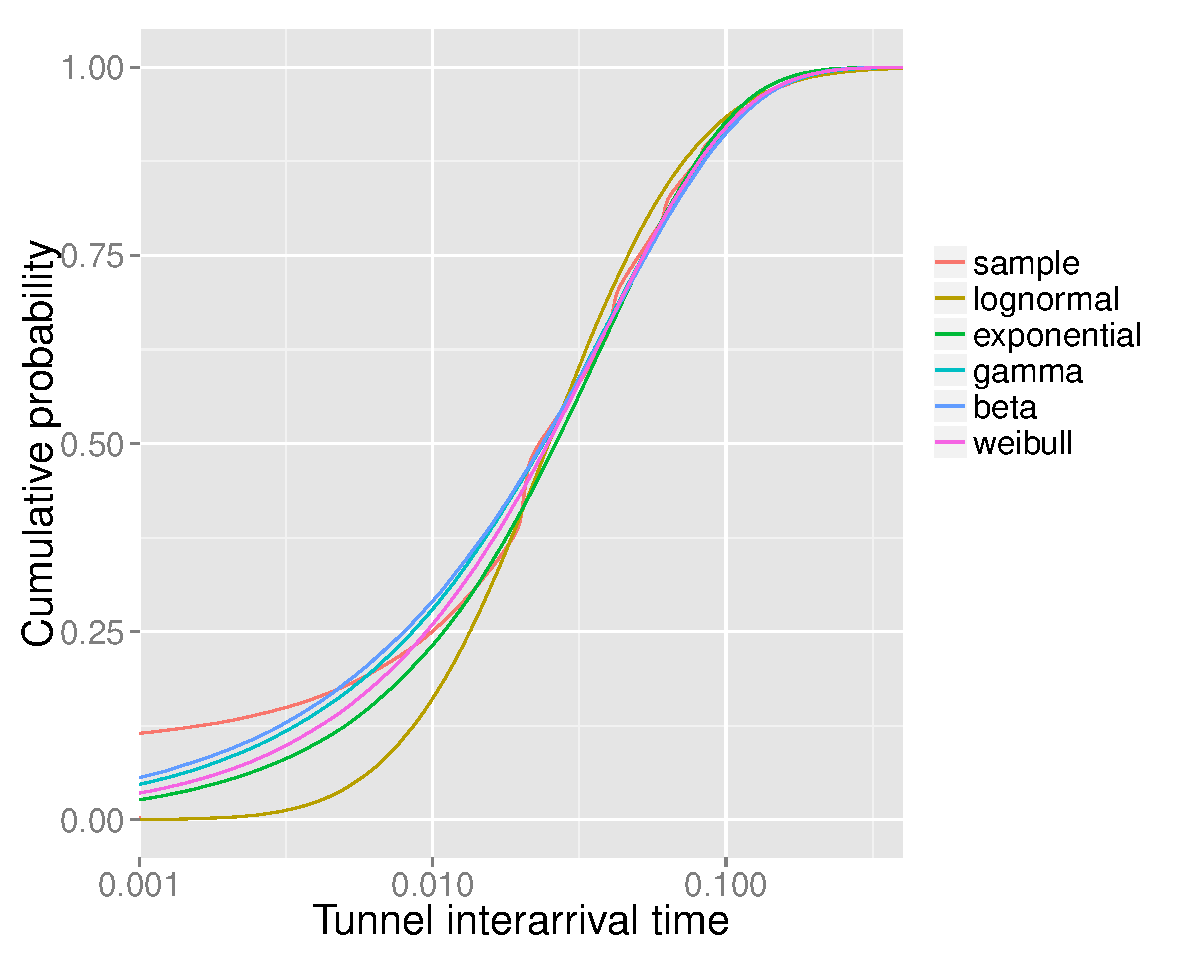
\includegraphics[width=0.9\textwidth]{images/R-IAT-ecdfs.pdf}
	\caption{Sampled inter-arrival time \acrshort{CDF} and fitted theoretical distributions.}
\label{c4:fig:IAT-cdfs}
\end{figure}

In order to investigate the tunnel \gls{IAT}, Figure~\ref{c4:fig:IAT-cdfs} displays the overall \gls{ECDF} with fits for various basic probability distributions. Each of the fits was generated through the method of moments matching.

The goodness of these fits was checked both visually using the \glspl{CDF} plots and numerically with goodness of fit measures, using Pearson's correlation coefficient and Pearson's $\chi^2$ test. Unfortunately, none of the probability distributions reaches the significance level for $\chi^2$. This can probably be largely attributed to the various previously described artifacts in the data. Matching them visually, the exponential fit seems to be reasonably close to the experimental data.

\begin{figure}[htb]
	\centering
	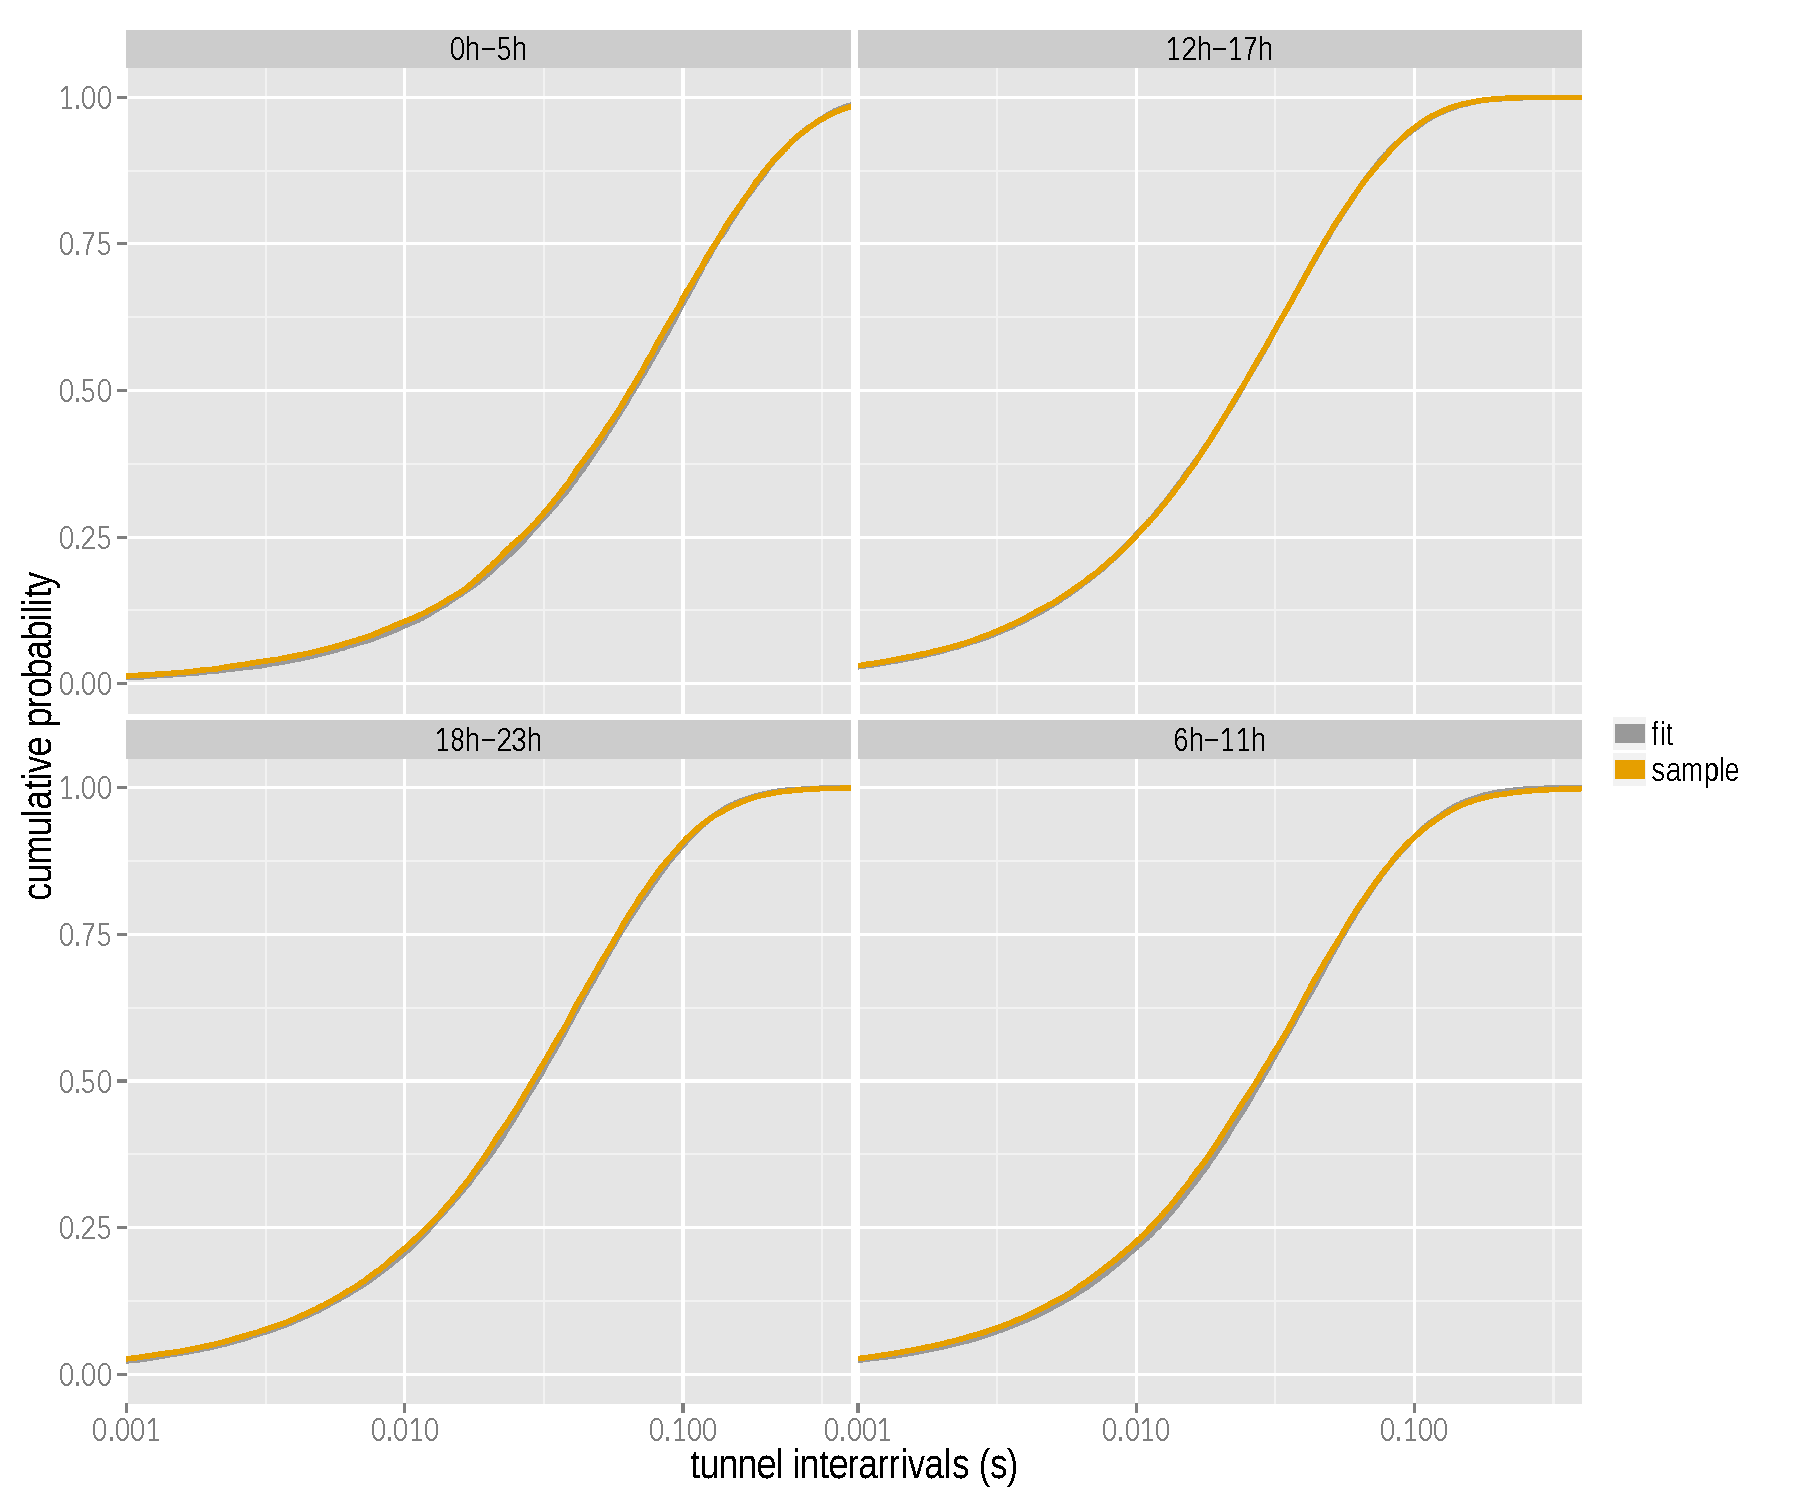
\includegraphics[width=0.9\textwidth]{images/R-IAT-active-fit-cdf-facets.pdf}
	\caption{Empirical and exponentially fitted \acrshortpl{CDF} of the tunnel \acrshort{IAT} by time of day. \acrshortpl{CDF} are overlapping as the coefficient of determination is close to $1$.}
\label{c4:fig:pdparrivalsecdf}
\end{figure}

To improve the fits, two modifications were made to the process. First, to remove the \SI{20}{\milli\second} steps, only the active tunnels were taken into consideration. Second, the overall \gls{IAT} distribution was once again split up into time of day slots. The overall distribution is just a superimposition of the individual slots anyway. Therefore, this should further improve the fidelity of the fits.

\begin{table}[htb]
\caption{Parameters for the exponentially distributed inter-arrival times and corresponding Pearson correlation coefficients.}
\label{c4:tab:IAT-fits}
	\centering
	\begin{tabu}{X[0.9,l]X[r]X[r]} 
	\toprule
	\textbf{Time of Day} & $\mathbf{\lambda}$ & $\mathbf{R_{arrival}}$\\ 
	\midrule
	0h-5h   & $10.67477$ & $0.995$ \\
	6h-11h  & $24.53298$ & $0.992$ \\
	12h-17h & $29.2504$  & $0.993$ \\
	18h-23h & $23.49983$ & $0.986$ \\
	\bottomrule
	\end{tabu}
\end{table}

The results are depicted in Figure~\ref{c4:fig:pdparrivalsecdf}. To improve plot visibility only four larger time slots are displayed here while the actual fits were conducted for each hour slot. Parameters for the exponential distribution $F(x) = 1- e^{-\lambda x}, x \geq 0$ and the corresponding correlation coefficients to the original data for the four time slots are given in Table~\ref{c4:tab:IAT-fits}. The fitted functions match the empirical data quite well, with some deviation present at the left tail but an overall positive correlation coefficient approaching $1$.


%%
\paragraph{Duration Fitting}

The second fitting effort surrounds the empirical data concerning the tunnel durations. However, none of the basic probability distributions (including exponential, gamma, and Weibull distributions) fit the tunnel duration even remotely. One of the reasons for this is probably that the tunnel duration is influenced by an overwhelming amount of factors, which were previously described. This superposition, especially with the user behavior, will result in unpredictable results that does not follow any basic probability distribution.

\begin{figure}[htb]
	\centering
	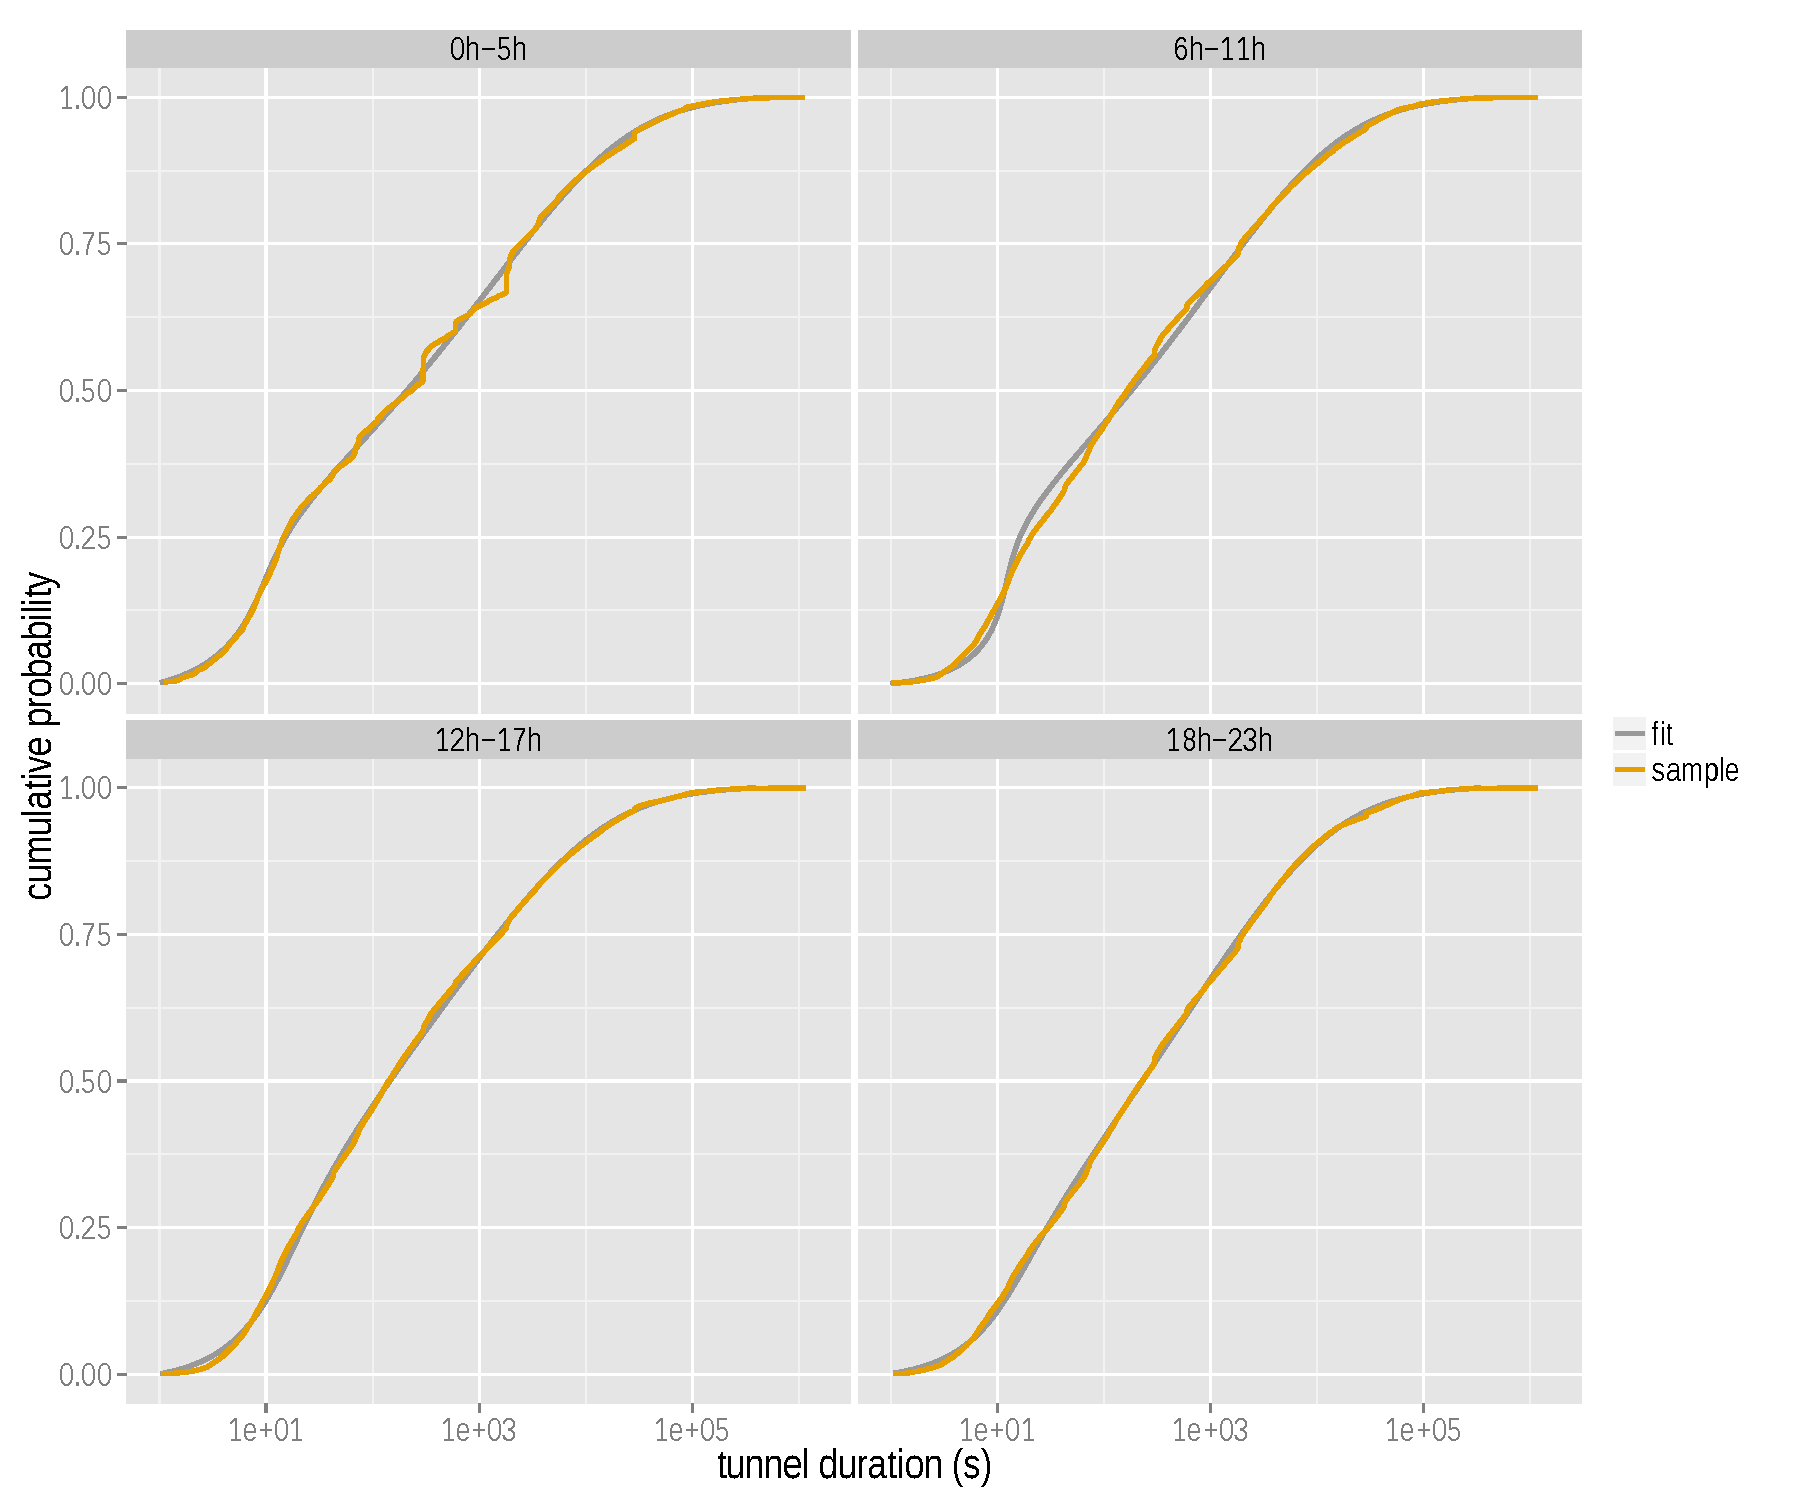
\includegraphics[width=0.9\textwidth]{images/R-duration-fit-cdf-facets.pdf}
	\caption{Empirical and fitted \acrshortpl{CDF} of the tunnel duration by time of day with fitted rational functions.}
\label{c4:fig:fittedsdurationlots}
\end{figure}

Instead, rational functions are fitted to the \glspl{ECDF} using the proprietary third-party tool \textit{Eureqa}~\cite{eureqa_paper, eureqa_software}. This allows for a much closer fit as seen in Figure~\ref{c4:fig:fittedsdurationlots}, but limits its application in the statistical evaluation.

\begin{table}[htb]
\caption{Inverse rational functions fitted to the \acrshortpl{ECDF} of the tunnel duration by time of day and correlation coefficients of the fit.}
\label{c4:tab:fits-duration}
	\centering
	\begin{tabu}{X[1.1,l]X[4.5,r]X[r]} 
	\toprule
	\textbf{Time of Day} & \textbf{Inverse Serving Time \gls{CDF} Representation} & $\mathbf{R_{dur}}$\\ 
	\midrule
	0h-5h & $0.919 - 60.614y - 3498.78y^3 - \frac{110.707y + 2289.94y^3}{y - 1.005}$ &  $0.999$ \\
	6h-11h & $1 + 117.484y - 368.643y^2 - \frac{1720.13y^4}{y - 1.004}$ & $0.999$ \\
	12h-17h & $0.953 + 69.491y + \frac{81146.1y^3 + 1.086\times10^6y^5}{805 - 802.01y}$ & $0.999$ \\
	18h-23h & $0.912 + 82.056y - \frac{2936.93y^4}{1.945y - 1.953}$ & $0.999$ \\
	\bottomrule
	\end{tabu}
\end{table}

	% high precision:
	% 0h-5h & $0.919208 - 60.6136y - 3498.78y^3 - \frac{110.707y + 2289.94y^3}{y - 1.00469}$ &  $0.999$ \\
	% 6h-11h & $1 + 117.484y - 368.643y^2 - \frac{1720.13y^4}{y - 1.0041}$ & $0.999$ \\
	% 12h-17h & $0.952566 + 69.4907y + \frac{81146.1y^3 + 1.08572\times10^6y^5}{805 - 802.01y}$ & $0.999$ \\
	% 18h-23h & $0.911924 + 82.0562y - \frac{2936.93y^4}{1.94468y - 1.9532}$ & $0.999$ \\

Table~\ref{c4:tab:fits-duration} contains the functions which were fitted to the \textit{inverse} \gls{CDF}. The inverse was chosen here to simplify the modeling and simulation process coming afterwards. The functions can be easily inverted again for other purposes. Both the \glspl{CDF} in the plot as well as the Pearson correlation coefficient, which again approach $1$, confirm the goodness of the fitted functions.


% \begin{table}
% \centering
% \caption{TAC Statistics}
% \begin{tabu}{|X|X|X[1.5]|X|X|X|} \hline
% & \textbf{\# of Flows} & \textbf{Total Traffic (Bytes)} &  \textbf{\# of Tunnels} & \textbf{\# of GTP Signalling Msgs} & \textbf{\# of Distinct IMSIs}\\ \hline
% Total          & 2234659247 & 122758578593993 (112TB)    & 16632094 & 409733865 & 1255293 (all) / 1030895 (with flows) \\ \hline
% In TAC DB      & 2228315260 & 122716712007150 (111.61TB) & 14565430 & 372662108 & 1015891 \\ \hline
% Smartphones    & 459990512  & 15721818747754 (14.30TB)   & 10030734 & 311342846 & 476675  \\ \hline
% Regular phones & 5705832    & 448140315058 (0.41TB)      & 897529   & 3860162   & 116124  \\ \hline
% 3G dongles     & 1487230062 & 92215931895630 (83.87TB)   & 2114756  & 39053819  & 315003  \\ \hline
% Android        & 241973565  & 7953178401958 (7.2TB)      & 2383255  & 177537567 & 175919  \\ \hline
% iOS            & 161408903  & 5481693567152 (5TB)        & 3145384  & 83374590  & 99679   \\ \hline
% Symbian        & 22827418   & 1332996529271 (1.21TB)     & 3520242  & 18479002  & 162790  \\ \hline
% Blackberry OS  &            & 128074907884 (0.12TB)      &          &           &         \\ \hline
% \end{tabu}
% \end{table}


%Devices with GTP signaling but no user plane traffic: (\#distinct imsis gtp db)-(\#distinct imsis flow db):
% $255293-1030895=224398\text{ or }17.88\%$

%%%%%%%%%%%%%%%%%%%%%%%%%%%%%%%%%%%%%%%%%%%%%%%%%%%%%%%%%%%%%%%%%%%%%%%%%%%%%%%%
%\subsection{Correlations to User Traffic}
% TODO, incl. measurements



%%%
% Direct signaling traffic overhead in relation to user traffic and induced network load

% GTP Header: 12 Byte
% IE header and footer: 2 Byte
% Maximum minimum data size including all \glspl{IE}: 221 Byte + 12 Byte Header + 2*37 Extension Header = 307 Byte
% Minimum size of message with just mandatory \glspl{IE}: 12 + 30 + 2*5 = 52 Byte

% 307 Bytes:
% calculation from our dataset
% Total maximum signaling traffic with this calculation: 117.15GB
% Ratio: 0.10\%
% 52 Bytes:
% Total maximum signaling traffic with this calculation: 19.84GB
% Ratio: 0.02\%
% Total traffic: 122758578593993


% signaling calc:
% gtp signaling traffic volume estimation $v_s$ = (1059B gtp message + 8B udp header + 20B ipv4 header) = 1087B * 409733865 number of request/response pairs * 2 (2 messages per pair) = 8,9076142E11B
% ratio to total $r=\frac{v_s}{v_t}=0.72\%$  $v_t=122758578593993B$


%%
%TODO: radio access type plots, if we have the data
% We do not.
%
%\begin{figure}
%\centering
%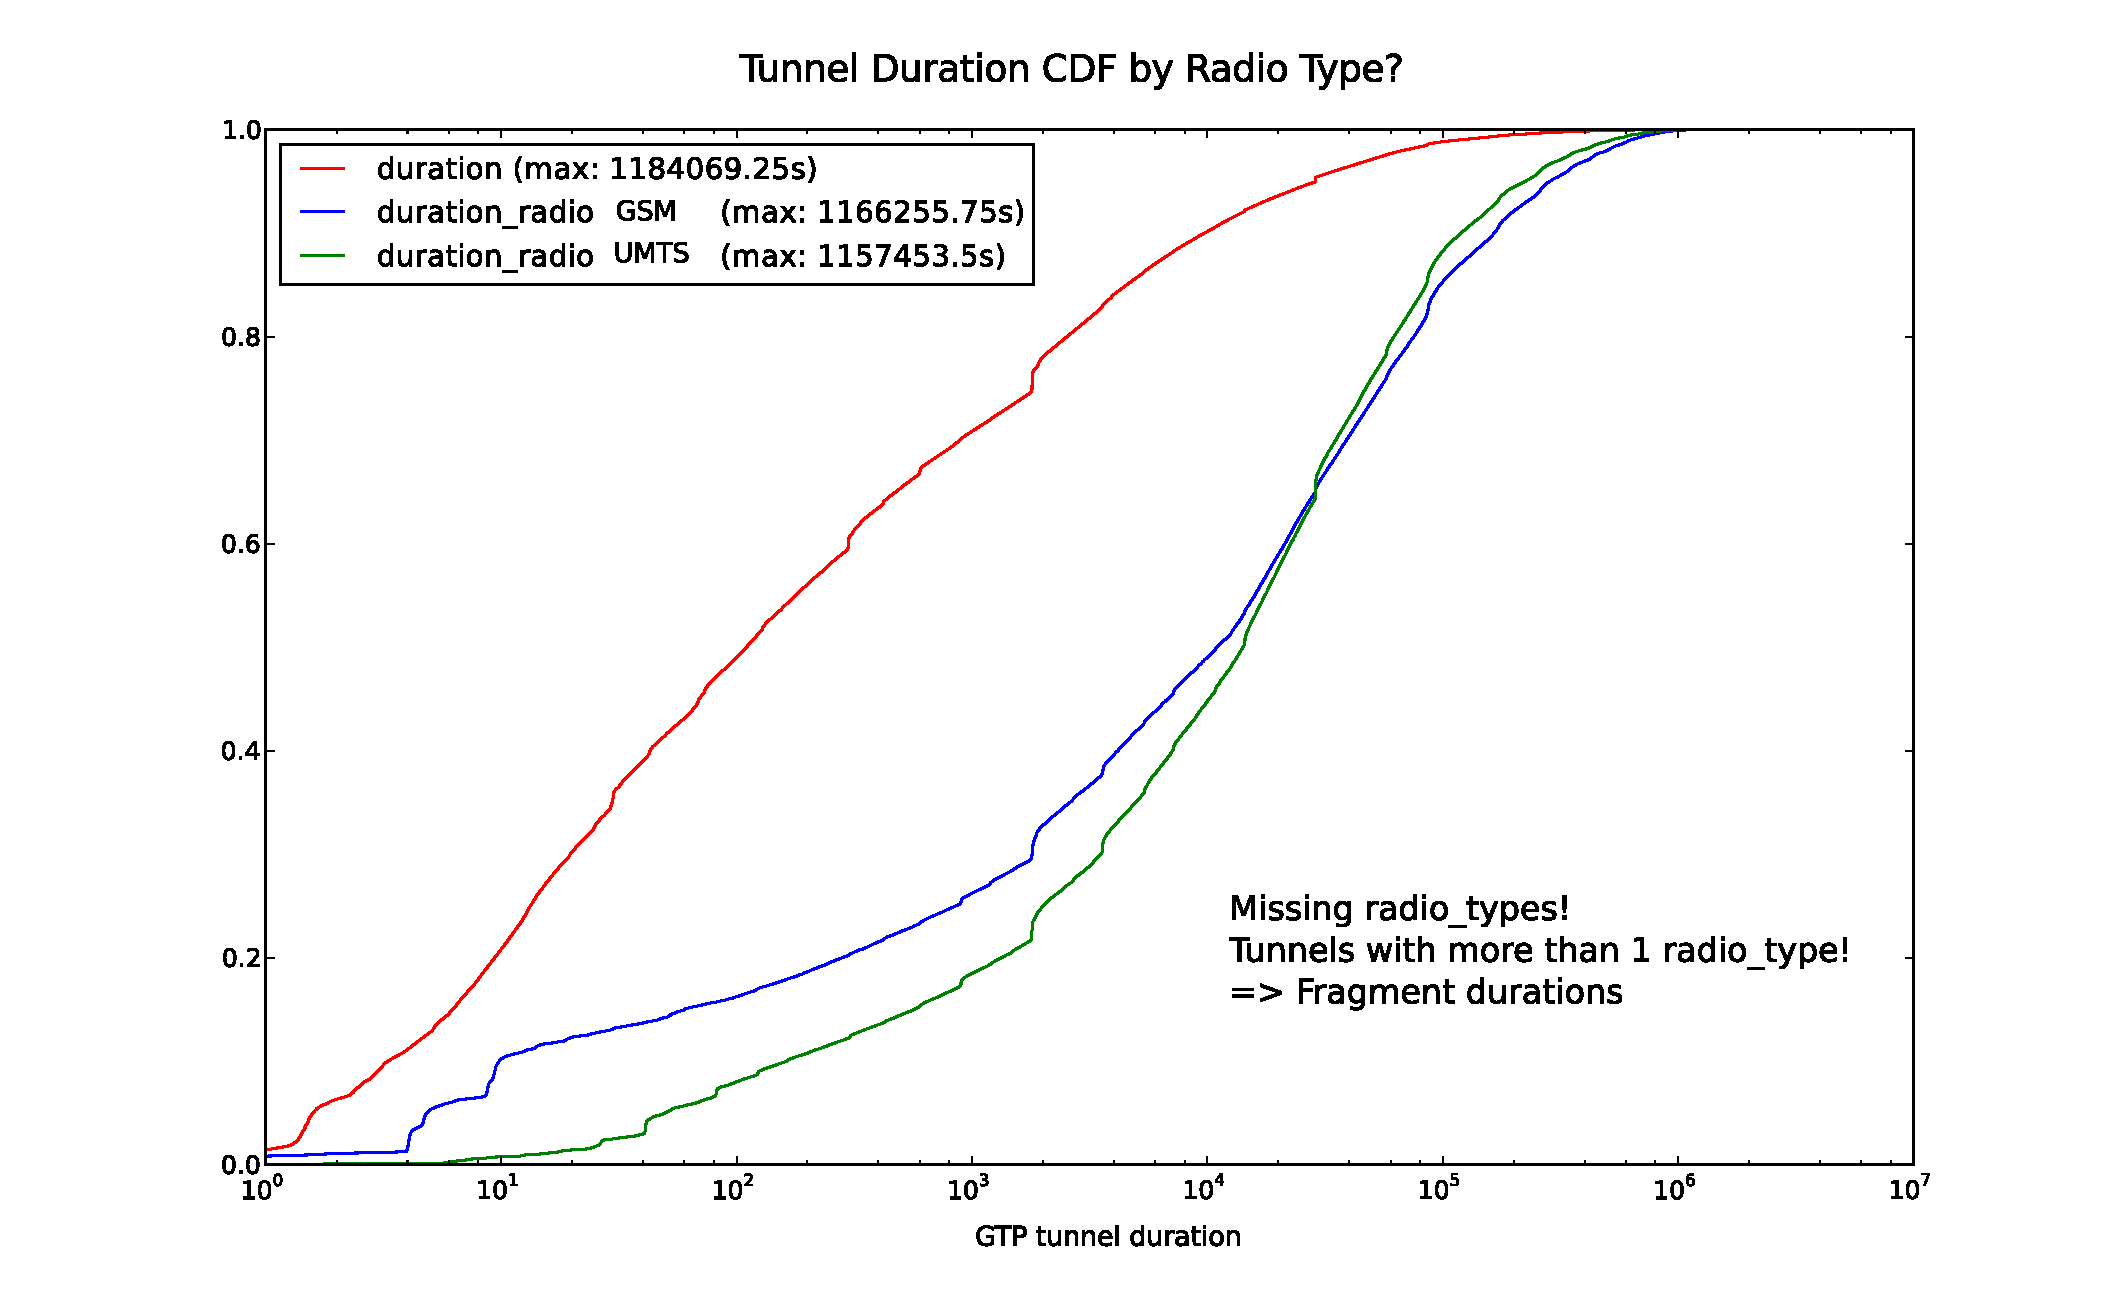
\includegraphics[width=\columnwidth]{figures/tunnel-dur-radio-cdf-mod.pdf}
%\caption{Tunnel duration distribution, separated for UMTS and GPRS radio access [NOTE: only in the last tunnel segment; and majority of radio types %is unknown anyway.}
%\label{fig:cdf-duration-radio}
%\end{figure}


%%%%%%%%%%%%%%%%%%%%%%%%%%%%%%%%%%%%%%%%%%%%%%%%%%%%%%%%%%%%%%%%%%%%%%%%%%%%%%%
%!TEX root = ../../dissertation.tex
%%%%%%%%%%%%%%%%%%%%%%%%%%%%%%%%%%%%%%%%%%%%%%%%%%%%%%%%%%%%%%%%%%%%%%%%%%%%%%%%
\section{Queuing Theory Basics}

\begin{itemize}
\item Kleinrock Queuing Systems Volume 1 \cite{Kleinrock:1975:TVQ:1096491}
\item Tran-Gia Analytische Leistungsbewertung verteilter Systeme \cite{trangia-lbvs}
\item Markov Models 
\item Solvability and Queuing Simulation
\end{itemize}


\subsection{Little's Law}
``A proof for the queuing formula: L= $\lambda$W'' \cite{little1961proof}

With $L$  as the number of customers in a stable system, the arrival rate of new customers $\lambda$ and the average time $W$ of a customer in the system this universal law states:

\begin{equation}
L = \lambda W
\end{equation}

\subsection{Kendall's Notation}

Kendall's notation is a naming and classification convention for queuing systems first defined by Kendall in in 1953 \cite{kendall1953stochastic} and later extended on. In its simplest form it reads \textit{A/S/s} with A denoting the arrival distribution, S the service time, and s the number of servers. One extended notation \textit{A/S/s-q}, the one we will use, additionally describes the queue length. With this, one can, e.g., easily distinguish between a queueing system ($q=\infty$) and a blocking or loss system ($q=0$). The most commonly used arrival processes and servie time distributions are summarized in Table~\ref{c2:tbl:kendalldistributions}.


\begin{table}[htbp]
	\caption{Typical abbreviation of processes in Kendall's notation.}
	\label{c2:tbl:kendalldistributions}
	\begin{tabu}{X[l]X[6]}
	\toprule
	\textbf{Symbol} & \textbf{Description} \\
	\midrule
	M & Markovian, i.e. Poisson, arrival process or exponential service time distribution\\
	D & Deterministic arrival process or service time distribution\\
	G & General arrival process or service time distribution with no special assumptions\\
	GI & General arrival process with independent arrivals; also called regenerative \\ 
	\bottomrule
	\end{tabu} 
\end{table}

The simplest queuing system is \textit{M/M/1-$\infty$}, which can also be described as a Markov chain and thus 

TODO: oder direkt M/M/n-$\infty$?

State probability, i.e. number of customers in the system
Blocking probability $p_B$ (for loss systems)


Following from Little's Theorem, the queue utilization $\rho$ is given as
\begin{equation}
\rho = \frac{\lambda}{\gamma}
\end{equation}

with $\lambda$ Poisson arrival rate, $\gamma$ exponential service time parameter


explain Erlang loss system and tractability


%%%%%%%%%%%%%%%%%%%%%%%%%%%%%%%%%%%%%%%%%%%%%%%%%%%%%%%%%%%%%%%%%%%%%%%%%%%%%%%%
%!TEX root = ../../dissertation.tex
%%%%%%%%%%%%%%%%%%%%%%%%%%%%%%%%%%%%%%%%%%%%%%%%%%%%%%%%%%%%%%%%%%%%%%%%%%%%%%%%
\section{Streaming Modeling}
\label{c3:sec:modeling}

As stated, the goal of this chapter is to model the measuring process and reliable streaming. This section will introduce our reliable \gls{TCP}-based streaming model. It is intended for easily comparing different protocol variants against each other and measuring all variants in one testbed. 

But first, because any evaluation of a model requires metrics, we describe ones appropriate to the model and give a rationale.
 
%%%%%%%%%%%%%%%%%%%%%%%%%%%%%%%%%%%%%%%%%%%%%%%%%%%%%%%%%%%%%%%%%%%%%%%%%%%%%%%%
\subsection{Metrics for Reliable Transport Streaming}
\label{c3:metrics}

When measuring anything related to video or even just image quality, one has the choice between conducting a subjective or objective assessment. 

During a subjective test, human assessors evaluate and rate video quality in a controlled environment with the results usually being aggregated into an overall relative quality score \gls{MOS}. Through the human element, conducting a subjective assessment is very time and resource consuming but it also achieves the highest precision.

This is where, objective video quality assessments come into play. Modern objective models attempt to recreate the features of the humans' visual perception and psychophysics and are calibrated by subjective assessments. Most objective models operate on a full reference approach, they directly compare the original reference video to the resulting video after being encoding or transmitted.

Two of the simplest full reference image quality metrics, which can also be applied on video, are the \gls{MSE} and \gls{PSNR}, defined as:

\begin{equation}
    \begin{aligned}
    MSE = \frac{1}{N} \sum_{i=1}^{N}(x_i - y_i)^2\\
    \text{and } PSNR = 10 \log_{10} \frac{L^2}{MSE},
    \end{aligned}
\end{equation}

with $N$ as the number of pixels in a frame and individual pixels $x$ and $y$ from the reference and output frame respectively. $L$ denotes the maximum value of a pixel. For grayscale or when investigating each color channel separately, usually $L = \SI{8}{\bit} = 255$.  \cite{objective-vqa}

Image quality models can by nature only test for spatial distortions of a single image. This includes a general blockiness or blurriness, noise, or reduced resolution. Dedicated video quality assessments can additionally take temporal metrics into account, e.g. frame rate anomalies. Such models are being researched and standardized by the \gls{ITU} and \gls{VQEG} for example in \cite{ituJ144, ituJ246, ituJ247}.


When conducting dedicated streaming quality measurements, only this portion should be taken into account by a metric, and not the initial encoding process. During streaming only a specific subset of quality degradations can occur. Lost or late packets can cause missing blocks in a frame or frames to be skipped completely. Initial thoughts concerning \gls{IPTV} \gls{QoE} have been given in \cite{ituG1080} and the influence of packet delay variations on playout buffers is investigated in \cite{rfc3393}The \gls{MDI} \cite{rfc4445} is an attempt to capture this behavior and relate it to the network \gls{QoS}. Its metric relies on two properties, the \gls{DF}, as a measure of the network's latency and jitter, and the media loss rate. Of special interest to this investigation is the \gls{DF}, which is calculated based on a virtual buffer (VB) of received stream data as

\begin{equation}
    \begin{aligned}
        VB = r_{rcv} - r_{drain} \\
        DF_i = \frac{\max(VB) - \min(VB)}{r_{drain}}
    \end{aligned}
\end{equation}
 
Reliable streaming has even less possibilities to degrade a video stream. Packets can not be out of order and loss is concealed by \gls{TCP}, meaning that the transmitted and the played video are identical. The only thing that can still happen, is portions of the video arriving too late to be played out at their intended point in time.
A potential reliable streaming quality assessment metric needs to keep track of the following properties:

\begin{itemize}
    \item The initial delay, which is the time delta between the start of the transmission and the start of the video play.
    \item The number and lengths of interruptions or stalls during playback.
    \item For adaptive streaming, the characteristics of the quality levels the video was played in. This includes the number of switching events and the duration of each level.
\end{itemize}

A concise metric covering all properties has not been defined yet. The \gls{CI} was defined in \cite{1498486} and used to determine quality in \gls{P2P} live streaming. It is defined as \enquote{the number of segments that arrive before or on playback deadlines over the total number of segments} and with this partly captures the stalling property. In \cite{5634160} and \cite{DBLP:journals/corr/SeyedebrahimiBP13} a so-called \gls{PI} is defined and evaluated. The definition $I_p = uv$ is simply based on the number of stalls $u$ and the average stall duration $v$. 

Generally, most research operates just directly on these three properties, which allows for the most freedom in usage scenarios. The streaming measurement model presented in the following section also works with the assumption, that only the three properties are of importance. The model assumes no special metric, the individual properties can be directly attained from the model. Though any metric could still be applied on the results.


%%%%%%%%%%%%%%%%%%%%%%%%%%%%%%%%%%%%%%%%%%%%%%%%%%%%%%%%%%%%%%%%%%%%%%%%%%%%%%%%
\subsection{Measurement and Playback Model}
\label{c3:model}

Parts of the model presentation is based on the author's previous work published in \cite{cs3518}, \cite{metzger2011delivery}, and \cite{6229739}. It is based on the desire to compare all in-the-wild variants of reliable streaming protocols in a simple and concise way. This is achieved by basing the model on the component that is common to all of the approaches: the playback buffer.

To display a video stream, an application needs to maintain a playback buffer of sufficient size to at least gather enough data to reconstruct one single atomic unit of playback such as a video frame.
From the perspective of a player application , a video consists of a sequence of atomic units, video frames and audio samples.
The application progressively decodes the video from a source and stores the units temporarily in a memory buffer before playing them. In reliable streaming, the buffer is filled by the payload from received \gls{TCP} segments a subject to the network \gls{QoS}. The process can be subsumed as:

\begin{equation*}
\mathit{buffer}(t) = \sum_{0}^{t} \text{data}_\mathrm{received} - \sum_{0}^{t} \text{data}_\mathrm{played}
\end{equation*}

Both the incoming and outgoing data stream are variable over time. The fill level of the playback buffer is the critical component in the playback process and the central element of the model.If the buffer reaches a size of zero the playback process stops and stalling occurs.

\begin{figure}[htb]
    \centering
    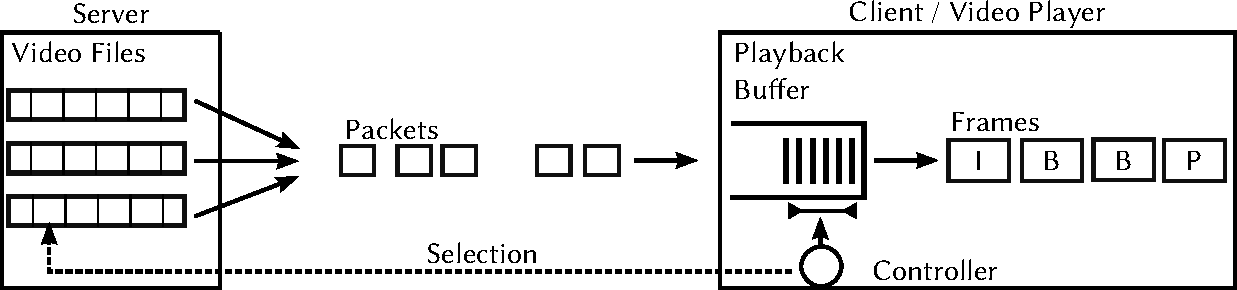
\includegraphics[width=0.9\textwidth]{images/playback-model.pdf}
    \caption{Reliable streaming playback model based on buffer control.}
    \label{c3:fig:playback-model}
\end{figure}

Figure~\ref{c3:fig:playback-model} overviews the reliable streaming model. The controller, part of the video player, selects a video from a remote location and the transmission is started, filling the playback buffer. The model has three degrees of freedom, which are all governed by the controller and together are coined playback strategies. These are:

\begin{itemize}
    \item The initial playback delay, which is the time between the initiation of the video stream transmission and the actual stream playback. The larger this is chosen, the bigger the safety margin on the buffer gets. If the video and transmission bitrate are known to be constant and and appropriately dimensioned, the initial delay can be chosen to be very small.
    \item Playback pause and resume decisions based on the current buffer fill level. This is a generalization of the initial playback delay, which is in fact only one, albeit always occurring stalling period.
    \item Selection of the video or video segment with a video bitrate chosen according to the current network throughput. This is only applicable for adaptive streaming.
\end{itemize}


These decisions yield a stalling period distribution for a streamed video. The frequency and the duration of stalls directly relate to the decision function of the playback model. The more frequent the stalls are, the shorter they will be; if the strategy produces longer stalls, they will be less frequent assuming the same network conditions. The time scale on which streaming applications buffer content usually lies in the range of seconds. This is a necessity in best-effort networks, as the available network bitrate might drop unexpectedly and cause stalling.


The the rest of this sections present fundamental playback strategies and strategy building blocks with features extracted from real world examples, which are given afterwards. 



%%
\subsubsection{Null Strategy}

The simplest strategy is having no strategy at all. Playback is started immediately when at least a single frame fully resides within the buffer and stops again at an empty buffer. The behavior can be summarized as ``Whenever anything can be played from the buffer, do so''.

This results in frequent stops and a large loss in playback continuity and will therefore not be used in practice. However, this strategy has some interesting theoretical properties, which is why it is mentioned here.
It minimizes total stalling time and the required buffer space. Moreover, it gives an upper limit for the number of stalls occurring\footnote{As a video frame is atomic, no other model could possibly stop the playback more often.}. Therefore, it can act as a baseline reference to assess the performance of other strategies.

\begin{figure}[htb]
    \centering
    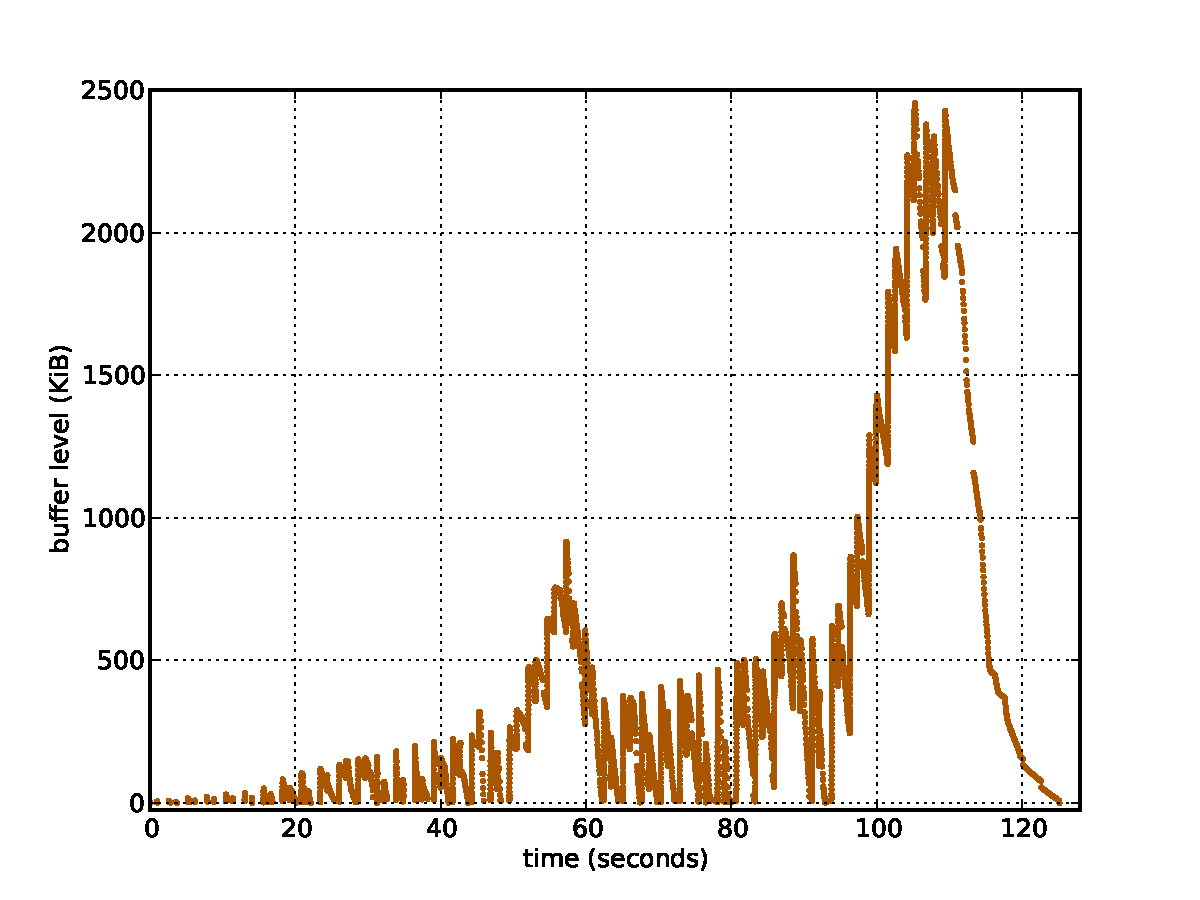
\includegraphics[width=0.9\textwidth]{images/bufferlevel-stall-new.pdf}
    \caption{Buffer fill level with null strategy; \SI{33}{\second} total stalling.}
    \label{c3:fig:bufferlevel-stall}
\end{figure}

Figure~\ref{c3:fig:bufferlevel-stall} depicts an exemplary time series diagram of the contents of a video buffer using this strategy with a transmission rate only slightly above the video stream's rate. The buffer frequently drops down to zero forcing a short stall. According to the presented related work on the \gls{QoE} impact of stalling frequency in comparison to the length of stalls \cite{6123395}, this is the worst possible scenario for a person watching the stream.


%%
\subsubsection{Threshold Strategies}

Instead of instantly restarting playback, a lower threshold can be introduced. Only after a certain buffer fill level threshold has been surpassed, playback will be started. Thresholds can be set independently for the initial playback delay and stalls, with the initial playback delay generally set to be higher.

The threshold can be chosen in a number of ways. It can either be an absolute data volume, a buffered video duration. The latter is much more suited for variable bitrate videos as it automatically adapts itself to the current bitrate. A third option is to buffer for a certain amount of real time -- this can be seen as threshold -- and starting playback after that period regardless of the volume of the buffer. Additionally, the threshold could also either be set to a constant value or dynamically chosen according to the expected network \gls{QoS}.

Besides this single-threshold strategy, a two-threshold strategy might make more sense for segment-based streaming. In addition to the lower threshold, an upper threshold is introduced. When reached, no new segments will be requested until the buffer arrives at the lower threshold again.  To achieve an hysteresis effect a third threshold, somewhere between the lower and upper bound, can also be introduced. Through this, the maximum buffer size can also be controlled. This is important in situations with hard limits on available memory. Mobile devices come to mind here.

\begin{figure}[htb]
    \centering
    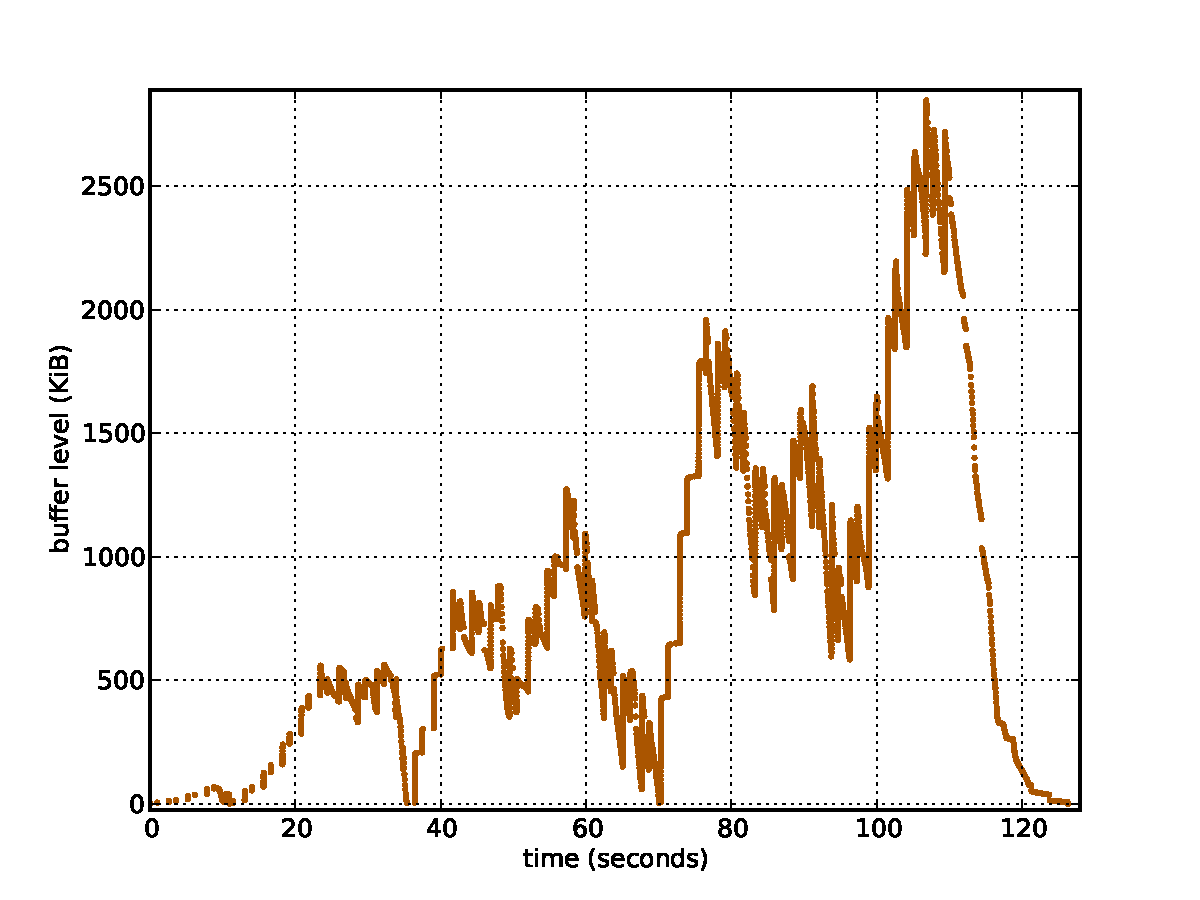
\includegraphics[width=0.9\textwidth]{images/bufferlevel-flash-new.pdf}
    \caption{Sample buffer fill level for a \SI{2}{\second} and \SI{5}{\second} buffered video duration threshold strategy; \SI{34}{\second} total stalling.}
    \label{c3:fig:bufferlevel-flash}
\end{figure}

An example buffer diagram is displayed in Figure~\ref{c3:fig:bufferlevel-flash}. In this case, the initial delay was controlled by a buffered video duration threshold of \SI{2}{\second} and a resume condition also based on buffered video duration but with a \SI{5}{\second} threshold. The strategy produces noticeable less stalls than the null strategy but slightly increases the total stalling time.


%%
\subsubsection{Pacing Strategies}

For segment-based \gls{HTTP} streaming, a two-threshold strategy is not the only supplemental option on top of simple streaming. Here, the controller can pace the request of future segments to match the overall, or the current video bitrate. A safety margin can also be factored in to even out short time fluctuations of either the transmission or the video bitrate. For example, the controller would request segments with an overall transmission rate of 1.25 times the video bitrate. The pacing rate can either be statically chosen in advance or can be calculated dynamically based on current or future conditions. The latter leads to predictive strategies.

%%
\subsubsection{Predictive Strategies}

In predictive strategies, knowledge of the future of the streaming process is used by the controller to adjust the start/stop and segment retrieval conditions. Instead of global knowledge, heuristics can instead attempt to approximate a future state.

A very simple predictive approach is to prolong the initial delay to the point, that no intermediate buffer underrun and thus no stall will occur. With global knowledge, the controller can start the stream at the earliest possible point in time, thus minimizing the total stalling time while still having only the initial delay.

\begin{figure}[htb]
    \centering
    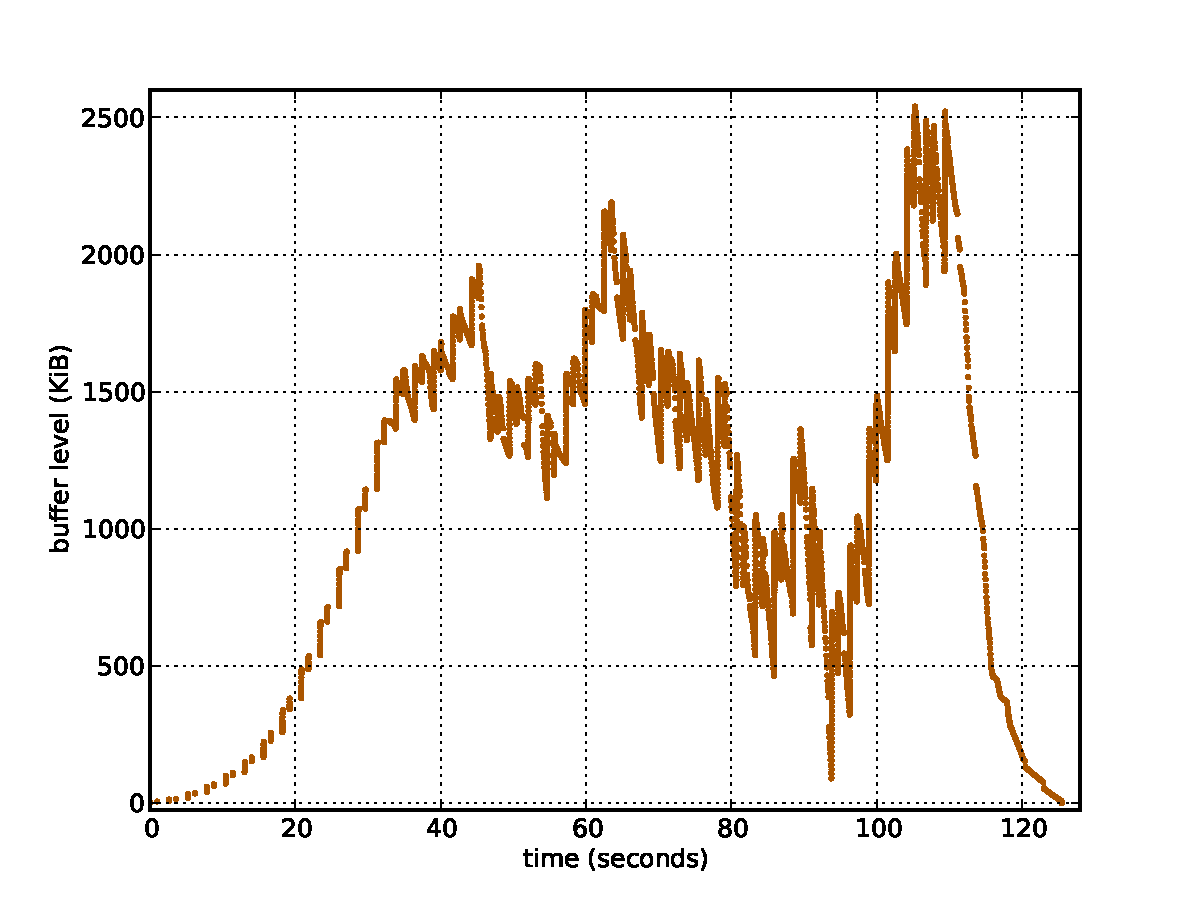
\includegraphics[width=0.9\textwidth]{images/bufferlevel-startdelay-new.pdf}
    \caption{Sample Buffer fill level for the delayed playback model, \SI{33}{\second} total stalling.}
    \label{c3:fig:bufferlevel-startdelay}
\end{figure}

Figure~\ref{c3:fig:bufferlevel-startdelay} depicts the time series of a sample implementation of this delayed playback predictive strategy with all necessary stalling occurring upfront.


%%
\subsubsection{Adaptive Strategies}

Most strategies for adaptive streaming are an extension of both the threshold as well as the pacing strategy. However, instead of a simple transmit-or-no-transmit ruleset, they can make much more fine-grained adjustments. The quality of the stream segment to be requested will be chosen, depending on the current fill level and drain rate of the buffer. This makes a trade off between maintaining a certain quality level and putting up with increased waiting times, and dropping the quality to a level sustainable at the current transmission rate.


\subsubsection{Real World Implementation Examples}

Actual streaming player implementations often do not implement only one of these strategies, but rather combine ideas from several. Herein, thresholds are often set arbitrarily through the implementor's best practices and not empirically evaluated, often making a trade-off between user perceivable quality and resulting server load. In general, every streaming service practically implements its own playback strategies. This section describes three example applications.

%%
\paragraph{2011 YouTube Flash Player Buffering Strategy}

Google's video streaming site YouTube is constantly changing its appearance and technical makeup. In recent years, YouTube streams are delivered by one of three players: The Website's Flash player, a browser-integrated HTML5-based player, or custom player implementations in mobile phones, set-top boxes and similar devices. Here, the Flash-based variant used in 2011 is described.

This player used a single threshold strategy with different threshold values for the initial delay and any subsequent stalls. The values were already described in Figure~\ref{c3:fig:bufferlevel-flash}. This model assumes sufficient network conditions in the beginning, requiring only a short initial playback delay to pre-fill the playback buffer. If, however, stalling occurs, then it will buffer longer to keep the stalling frequency down.

\begin{table}[htb]
    % increase table row spacing, adjust to taste
    %\renewcommand{\arraystretch}{1.3}
    \caption{Transmission Related Parameters from YouTube's Video URL Setup}
    \label{c3:tbl:yturl}
    \centering
    \begin{tabu}{|X[l]|X[p]|}
        \hline
        URL Part & Description \\ \hline
        \texttt{v$\alpha$.lscache$\beta$.c.youtube.com} &  Cache server involved in the delivery.\\
        \texttt{algorithm=throttle-factor} and \texttt{burst=40} and \texttt{factor=1.25} & Indicates initial burst plus block sending configuration. \\
        \texttt{ratebypass=yes} & Parameter to indicate no rate limiting.\\ \hline
    \end{tabu}
\end{table}

Furthermore, YouTube employs a proprietary pacing mechanism outside of the control of the streaming player. This is hinted at in the encoding of the \glspl{URL} of the video files and enforced by the video file cache server. Some of those not user-changeable parameters are described in Table~\ref{c3:tbl:yturl}. The pacing was in effect for all videos below high definition resolution, but has since then been extended to include all video files. 

\begin{figure}[htbp]
% used yt-delay/hPUGNCIozp0_delay_100 2, spyder with matplotlib config patch
    \centering
        \begin{subfigure}[b]{0.90\textwidth}
                \centering
                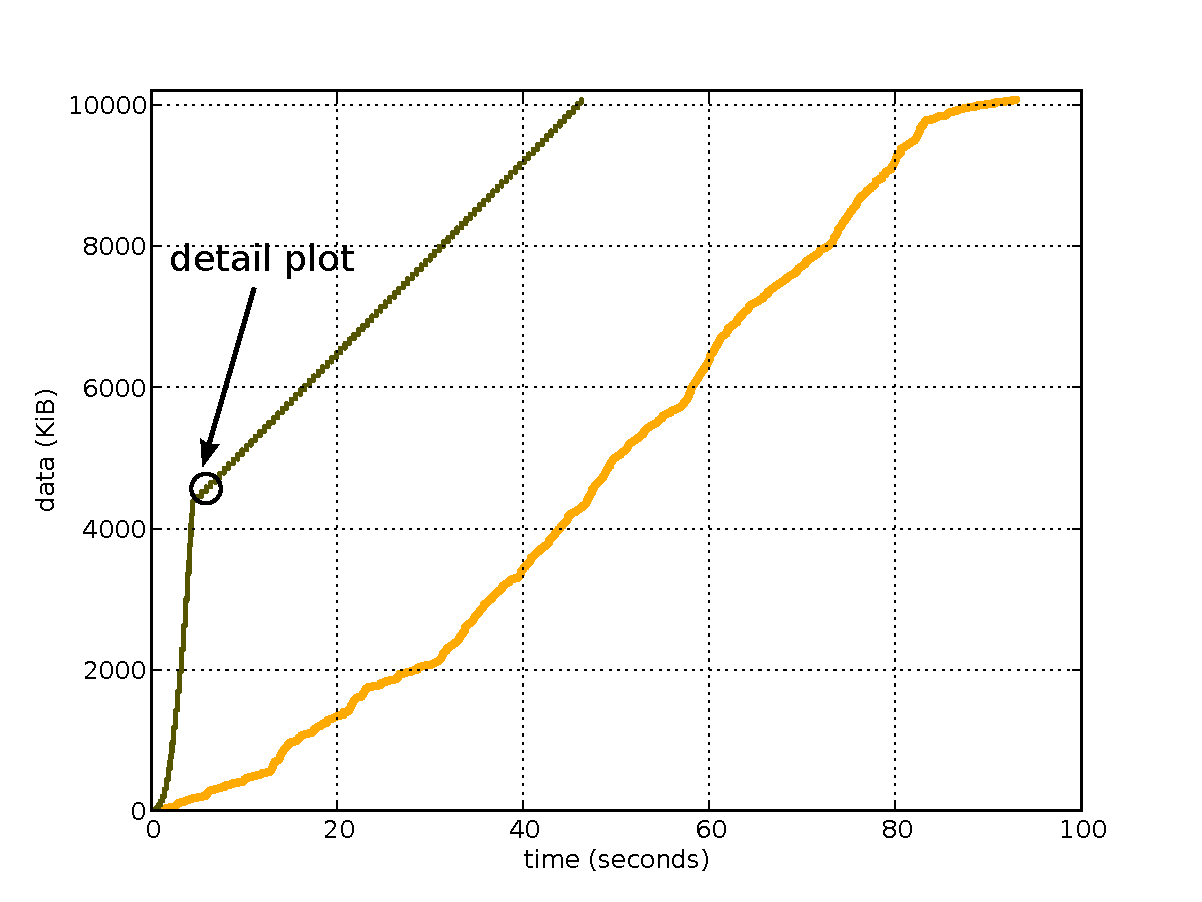
\includegraphics[width=\textwidth]{images/blocktransfer-mod.pdf}
                \caption{Overall graph.}
                \label{c3:fig:blocktransfer-overall}
        \end{subfigure}

        \begin{subfigure}[b]{0.90\textwidth}
                \centering
                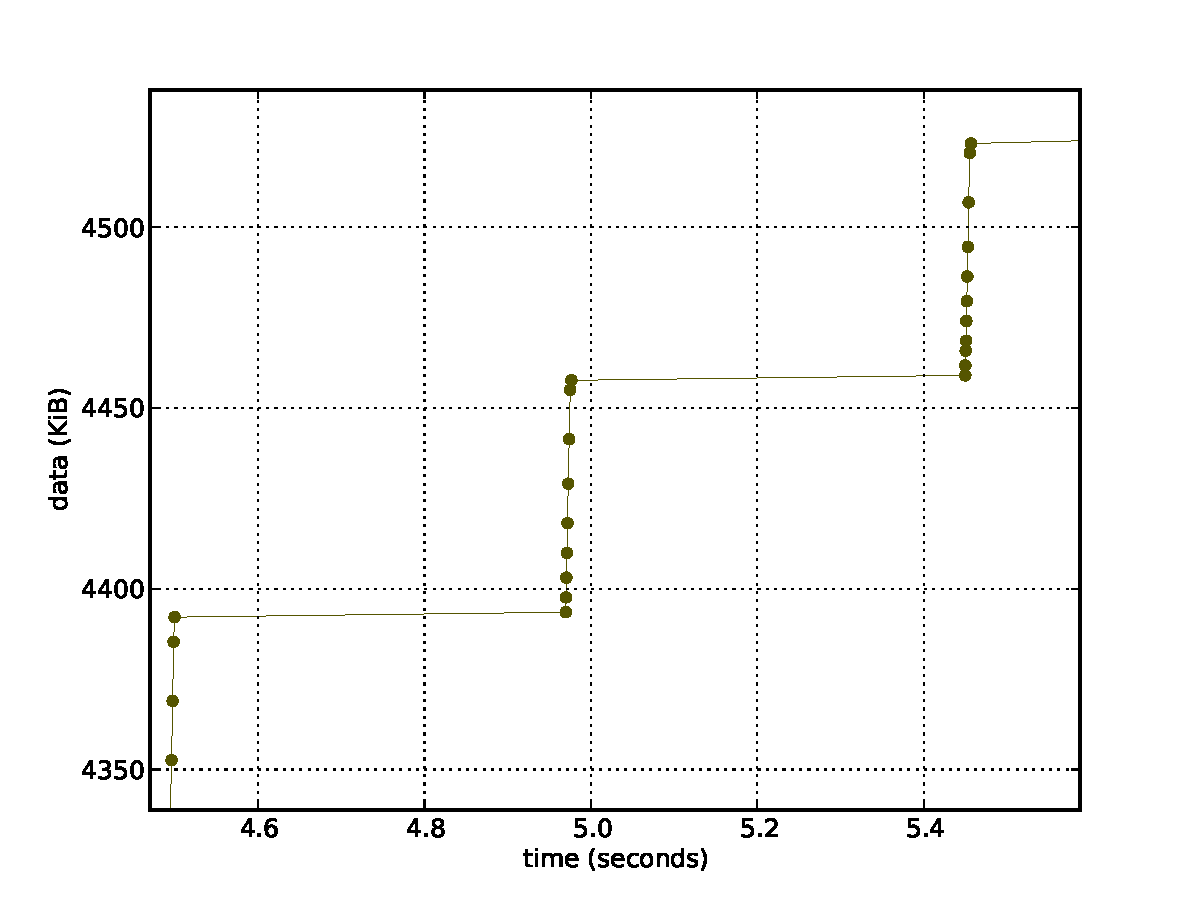
\includegraphics[width=\textwidth]{images/blocktransferdetail.pdf}
                \caption{Detail plot of the rate-limited block-sending phase.}
                \label{c3:fig:blocktransfer-detail}
        \end{subfigure}
\caption{Comparison of downloaded and consumed data volume revealing the pacing mechanism used by YouTube.}
\label{c3:fig:blocktransfer}
\end{figure}


The throttling method, also observed in \cite{alcock2011afcyt}, limits the transmission to a rate slightly above the average media bitrate, measurements and the \gls{URL} scheme indicates this to be a factor of the video bitrate of $1.25$. The rate limit is not constant, instead a ON-OFF block-sending scheme is facilitated. The scheme transmits short packet bursts, typically \SI{64}{\kibi\byte} in size, followed by long pauses as seen in Figure~\ref{c3:fig:blocktransfer}. The pause length between two bursts is set dynamically to reach the targeted bitrate on a larger time scale. The initial phase of the stream transmission is conducted unthrottled at line speed, presumably to allow for some pre-buffering to occur at the client media player. A possible reason for this server-side pacing is to avoid load spikes, with the added side effect of keeping the clients' buffer sizes in check.



%%
\paragraph{Firefox's HTML5 Player Strategy}

Video streaming can also be directly conducted with the Web browser, through the use of a HTML5 canvas element. The \gls{W3C} specifies the default technical process of HTMl5 video streaming in \cite{html5video} and essentially suggests a predictive strategy. Herein, the Web browser should estimate and correlate the transmission rate to the video bitrate. A property called ``autoplay'' uses this definition to start  playback of the associated video \enquote{as soon as it can do so without stopping}. The HTML5 strategy also allows to limit the buffer size through transmission pacing, negotiated with the server, and appropriately timed range requests.

The open-source Firefox browser represents an implementation of this specification and substantiates it further. The description of this strategy is based on Firefox's version 4.0 released in March 2011. Because it is an online algorithm which does not have global knowledge of the video and transmission speeds of any point in the future it has to estimate these.
To estimate the current and future rates, the moving average of the transmission rate $s_{MA}$ and the video bitrate $v_{MA}$ are calculated. The condition $c$ Firefox uses to start and resume the playback process is given in Algorithm~\ref{c3:alg:firefox}, with the buffered video duration $b_b$, and the duration spent buffering $b_T$.

\begin{algorithm}[htb]
    \centering
    \begin{algorithmic}
        \IF {$s_{MA} > v_{MA}$} 
          \STATE $c \gets ( b_b=20s \lor b_T=20s )$
        \ELSE
          \STATE $c \gets ( b_b=30s \lor b_T=30s )$
        \ENDIF 
    \end{algorithmic}
    \caption{Firefox playback (re-)start decision algorithm.}
    \label{c3:alg:firefox}
\end{algorithm}

 \begin{figure}[htb]
    \centering
    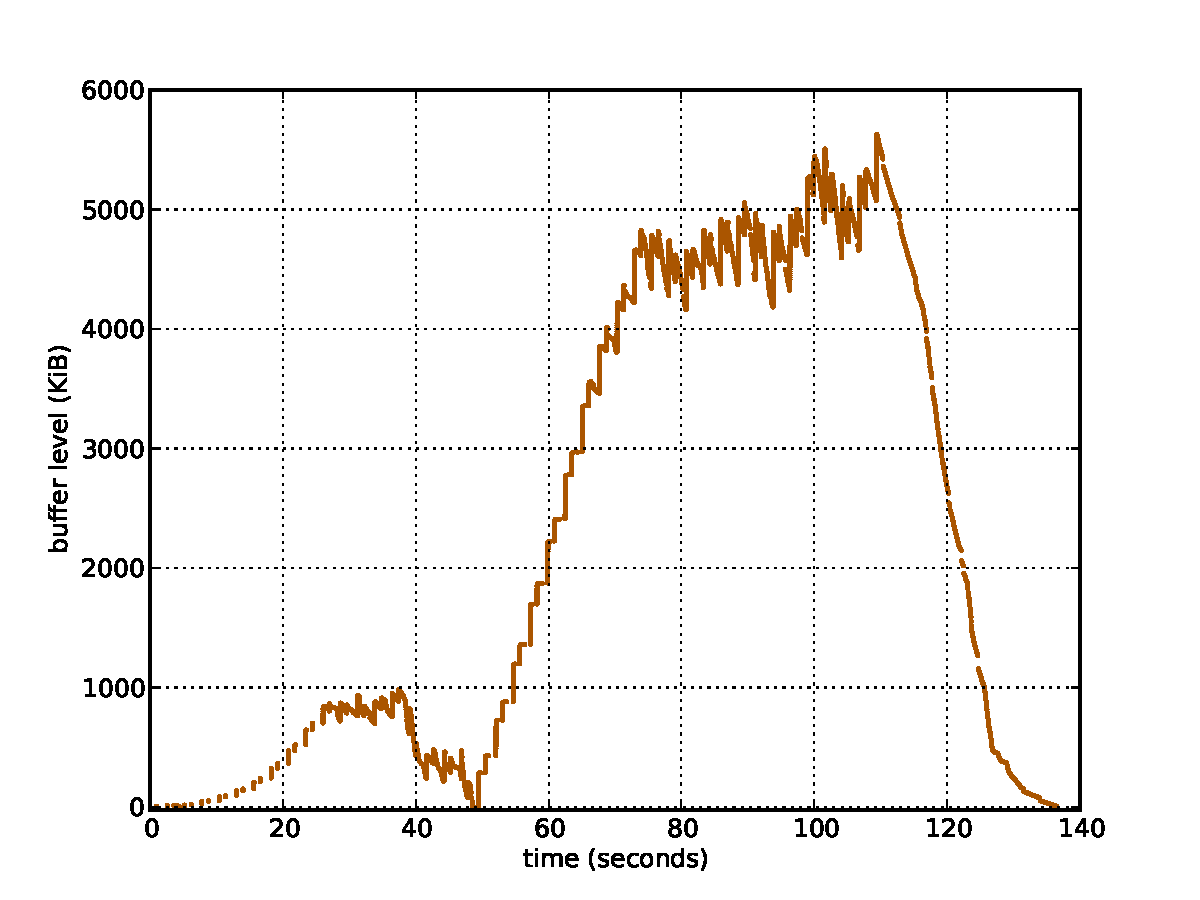
\includegraphics[width=0.9\textwidth]{images/bufferlevel-firefox-new.pdf}
    \caption{Sample buffer fill level for the Firefox 4 strategy, \SI{44}{\second} total stalling.}
    \label{c3:fig:bufferlevel-firefox}
\end{figure}


This approach is quite conservative and trades off long stalling periods for fewer stalls. The test case for our model is shown in Figure \ref{c3:fig:bufferlevel-firefox}. The playback starts only after a long waiting period and intermittent stalls cause a long buffering period. 
Due to the longer overall stalling time the player needs to buffer more data than other strategies. This may make it unsuitable for devices with sparse amounts of memory, e.g. mobile phones. On the other hand, could a large buffer also increase the chance of continuous playback in such scenarios with bad \gls{QoS}.


\paragraph{Adaptive streaming strategies}

Implementations for adaptive streaming players are again mostly proprietary and their behavior has to be derived from measurements. This is even true for adaptive streaming protocols, which have open specifications as these generally do not specify the player's behavior.

Microsoft's Silverlight player's strategy is described in \cite{BLTJ:BLTJ20505}. It employs a two-threshold model and rate estimations. When on of the thresholds is reached, the quality will be adjusted by one step upwards or downwards as long as the transmission rate is sufficient.

The buffering behavior of further protocol variants, including Adobe's \gls{HTTP} Dynamic Streaming, Apple's \gls{HTTP} Live Streaming and a sample implementation of \gls{DASH}, are investigated in \cite{Muller:2012:EDA:2151677.2151686,akhshabi2011experimental}.




% \begin{itemize}
% \item The player has been buffering data for at least 30 seconds.
% \item The player has already buffered an amount of data corresponding to 30 seconds of video.
% \item The video download has been completed.
% \item The moving average of the transmission rate is larger than the moving average of the video bitrate and the player has a safety buffer with 20 seconds of video data.
% \end{itemize}

% \begin{table}[htb]
%     \caption{Variables involved in buffering decisions.}
%     \label{c3:tbl:buffvars}
%     \centering
%     \begin{tabu}{|l|X[p]|} 
%     \hline
%     Variable & Description \\ \hline
%     $s_{MA}$ & Moving average of the transmission speed. \\
%     $v_{MA}$ & Moving average of the video bitrate. \\ 
%     $c$   & Condition upon which to start/resume playback. \\
%     $b_b$    & Amount of video data the buffer contains. \\
%     $b_T$    & Amount of time spent in non-playing buffering state. \\ \hline
%     \end{tabu}
% \end{table}

% used yt-delay/hPUGNCIozp0_delay_2500 1, spyder, color #aa5500
% data
% start delay 33s 
% flash 33.82s
% stalling 32.68s
% html5 as implemented in firefox 44s


%Which offers better quality to users? Some approaches (TODO: refs and explain how)

% Longer waiting time but very few stops. Stalling model definitely the shortest waiting time but stops too frequent with insufficient network conditions, i.e. can not really be used. Delayed playback requires total knowledge not available beforehand. Can maybe used with reduced information, bandwidth estimation, but this is essentially HTML5/Firefox.




%``application comfort'' time to skip, ...
%\subsubsection{Unreliable Streaming Metrics}
%... and why they mostly do not work / are not applicable.




%%%%%%%%%%%%%%%%%%%%%%%%%%%%%%%%%%%%%%%%%%%%%%%%%%%%%%%%%%%%%%%%%%%%%%%%%%%%%%%%
\section{Summary}
\label{c4:sec:conclusion}


In this paper, we took a look at the signaling behavior of devices in an operational \gls{3G} mobile network providing Internet access. Our focus does not lie on the wireless or user-oriented parts of the network, but on signaling in the core network. To the best of our knowledge, this paper is the first to offer an in-depth core network perspective on signaling. We give a \gls{GPRS} and \gls{UMTS} network primer, and introduce \gls{gtp} tunnel management, explaining the causes and actions within the network. Our evaluation is based on a week long data set acquired in the core network of an Austrian mobile operator.

% We now go back to the case of Angry Birds which was much quoted for causing excessive radio signaling at one point in time. 


In our observation of core network signaling involving \gls{PDP} Contexts and their management, we looked at the effect of device types and operating systems on the duration of \gls{gtp} tunnels. We can conclude that the distribution of tunnel durations in our evaluated dataset is dominated by smartphones. This is contrary to the conventional idea that a larger volume of user plane traffic also leads to an increase of signaling. In our dataset, this would mean that 3G dongles would cause most signaling, which is definitely not the case. Our paper shows that operators can determine which type of device has the most influence on the current network infrastructure by looking at and comparing tunnel duration distributions.

In this aspect, our findings support the stories of the casual game ``Angry Birds'' causing signaling storms in mobile networks by frequently downloading small ads, each small download resulting in disproportionate amounts of signaling load being generated. We conjecture from our results that measures taken to improve the radio interface control plane such as Fast Dormancy can have the converse effects in the core, as they could increase the tunnel churn.


All in all, our paper shows that operators can determine which type of device has the most influence on the current network infrastructure by looking at and comparing tunnel duration distributions. %Moreover, if a load situation occurs in the core network, the operator can decide which devices are the root cause and take appropriate measures. 
This investigations can also lead to better network planning that is more aware of the control plane by providing the necessary tools to identify probable causes for control plane activity. Lastly, we hope to raises some awareness with programmers about the potential unintended side effects their application traffic patterns can cause.

This paper serves as an introduction to the topic of the 3G core network control plane, and therefore provides only some initial insights into the actual signaling dynamics. Therefore, we would like to expand our evaluations, as there are several  angles not investigated so far that could prove worthwhile.

To get a grasp of the imposed load on the network as well as the involved network nodes, a calculation of the sizes of the tunneling messages was already hinted at. To improve on this naive attempt, actual numbers on the message sizes and involved \glspl{IE} could be recorded in future traces. Having correct signaling traffic volume data still does not reveal the processing load on core network elements. We plan to improve our methodology in this respect by taking at a look at how long it takes for the gateway nodes to process \gls{gtp} messages with respect to the current amount of user traffic and signaling. \gls{gtp} tunnels also cause a certain amount of overhead through additional headers and potential fragmentation of the user traffic, providing another investigation venue for the future (albeit more oriented towards user-plane IP traffic). 

Furthermore, besides the device-based classification, a differentiation based on the user traffic dynamics and correlation to signaling is planned. When looking closer at specific users, the mobility behavior also comes to mind. To investigate this, we intend to take a closer look at the occurring tunnel update messages as evidence, amongst others for mobility.

We also look forward to searching for multiple active tunnels per device. As discussed previously, the \textit{Secondary PDP Context Activation Procedure} enables devices to establish up to ten additional tunnels attributed with a different, higher QoS level, if the network supports this. The additional load of managing and holding multiple tunnels plus the displacement of other, ``lower-quality'' traffic could prove to be an interesting investigation. Initial observations indicate that this feature is rarely used today by very few types of devices, but it will be of increased interest in the face of ongoing LTE/EPS deployments, whose specifications expand upon this secondary tunnel concept.

For additional load investigations we also looked at the inter-arrival and processing time of tunnels and found further evidence of radio and diurnal effects influencing the core network. With this data in mind, an initial M/M/$\infty$ queue was created to model load occurring at the \gls{GGSN} with simple stationary analysis. This also serves a basis for future more detailed models.

We think that this investigation and load modeling can lead to better network planning: Being more aware of the control plane provides the necessary tools to identify probable causes for control plane activity. We would also like to expand our evaluations, as there are several angles not investigated so far that could prove worthwhile. This includes an examination of the exact number and size of signaling messages flowing through the core, a more detailed picture of the processing load these messages induce at the \gls{GGSN}, and an evolved model. Furthermore, a differential analysis of our data compared to a newer dataset (potentially including \gls{LTE} access) could really prove worthwhile.



%%%%%%%%%%%%%%%%%%%%%%%%%%%%%%%%%%%%%%%%%%%%%%%%%%%%%%%%%%%%%%%%%%%%%%%%%%%%%%%%
%%% MMB2014 Conclusion Starts here
In this paper we investigated trade-offs when virtualizing components of the mobile core network.

To this end, we first discussed a novel approach to mobile core network load modeling based on the control plane load at the \gls{GGSN}. The M/G/$c_c$ loss model is based on the currently implemented state of the network architecture and can serve as a baseline reference to plan and dimension one's own mobile network accordingly, not just based on expected user traffic as traditionally. To improve scaling in the future, we proposed a completely new and virtualizable approach to a \gls{GGSN}'s makeup.

Then, we presented random variables to model load in a \gls{GGSN} based on measurement data from the network of a nation-wide mobile service provider and made them available for reuse by other researchers.

Finally, we evaluate the model using a queing simulation. We have shown, that the system's blocking probability is roughly equal to the single-server model but in addition achieves large efficiency gains, even with very simplistic provisioning conditions and very long boot times. The model also has the ability to very easily scale out one's infrastructure by simply adding more small servers, reducing operational overhead. This might even lead to a new GGSN-as-a-Service business models, removing the need to provide and operate large amounts of infrastructure for rare cases of peak load. 
In the future we would like to deepen our modeling efforts to provide more dimensioning options for a core network. Also, we want to further investigate the correlation of user traffic and signaling and take a look at the implications specific traffic types bring for the core network. 